\documentclass[11pt,a4paper,titlepage,oneside]{report}
\usepackage{titling}
\usepackage{graphicx}
\usepackage{mathtools}
\usepackage{lmodern}
\usepackage{amsmath}
\usepackage{float}
\usepackage{subfig}
\usepackage{listings}
\usepackage[hidelinks]{hyperref}
\usepackage{url}
\usepackage[backend=biber]{biblatex}
\usepackage{makecell}

\addbibresource{bibtex.bib}

%% Memoir layout setup

%% NOTE: You are strongly advised not to change any of them unless you
%% know what you are doing.  These settings strongly interact in the
%% final look of the document.

% Dependencies
\usepackage{bfhlogo}
\usepackage{etoolbox}% http://ctan.org/pkg/etoolbox

\makeatletter
%%begin novalidate
%% Titlepage adjustments
\pretitle{\vspace{0pt plus 0.7fill}\begin{center}\Huge}
\posttitle{\end{center}\par}
\preauthor{\par\begin{center}\let\and\\\Large}
\postauthor{\end{center}}
\predate{\par\begin{center}\Large}
\postdate{\end{center}}
%%end novalidate
\def\@advisors{}
\newcommand{\advisors}[1]{\def\@advisors{#1}}
\def\@department{}
\newcommand{\department}[1]{\def\@department{#1}}
\def\@thesistype{}
\newcommand{\thesistype}[1]{\def\@thesistype{#1}}

\renewcommand{\maketitlehooka}{\noindent\bfhlogo[2cm]}

\renewcommand{\maketitlehookb}{\vspace{1in}%
  \par\begin{center}\Large\sffamily\@thesistype\end{center}}

\renewcommand{\maketitlehookd}{%
  \vfill\par
  \begin{flushright}
    \sffamily
    \@advisors\par
    \@department, BFH
  \end{flushright}
}

% Fix the chapters (unnecessary space)
\patchcmd{\@makechapterhead}{\vspace*{50\p@}}{}{}{}% Removes space above \chapter head
\patchcmd{\@makeschapterhead}{\vspace*{50\p@}}{}{}{}% Removes space above \chapter* head

\makeatother

\setlength{\droptitle}{-48pt}


\setlength{\parindent}{0pt}

\title{Open Source SLAM Library for Embedded Systems}
\author{Stefan Eichenberger\\<eichest@gmail.com>}
\date{January 2020}
\advisor{Prof. Marcus Hudritsch}
\expert{Dr. Harald Studer (Optimo Medical AG)}
\department{TSM CPVR Lab}

\lstset{
  basicstyle=\ttfamily\scriptsize
}

\begin{document}

\maketitle
\begin{abstract}
  Simultaneous location and mapping (SLAM) is a technology used for robot navigation and augmented reality. Today most SLAM libraries are proprietary or not ready for embedded systems. In this thesis, we write and analyse a library which is open source and usable on embedded devices.
\end{abstract}

\section*{Executive Summary}
Today we use Simultaneous Location and Mapping (SLAM) for robot navigation and augmented reality. Often these algorithms need a high performance graphics card or a high performance processor. For industrial and robotics purposes we face constraints in space, temperature and power consumption. Therefore, we use devices with less power consuming CPUs, which in turn are less powerful. In this thesis, we implement and analyse an algorithm called SVO which is capable to run on embedded devices. The reference implementation uses monocular cameras, while we use a stereo camera. We show that the algorithm is based on optical flow, a well-known principle in computer vision. The implemented algorithm performs 4 tasks. First it maintains a 3D point cloud which is used to estimate the camera pose. Second it performs a pose estimation based on the 3D cloud. We call this sparse image alignment. It uses a changed version of optical flow, which directly outputs a pose instead of a warp matrix. Third, to make the guess more accurate, it refines the pose by using standard optical flow, followed by a minimization of the re-projection error. Finally, in a last step, the algorithm performs a 3D point cloud update where it refines the cloud by taking the new pose into account.\\
We show that the algorithm works as outlined and can estimate the 3D pose as described by the authors of SVO. We see that the algorithm performs faster than a comparable SLAM algorithm called ORB SLAM. However, the current implementation is less accurate than ORB. We conclude that SVO shows great promise as a SLAM algorithm for embedded devices.

\tableofcontents

\chapter{Introduction}

Humans use different sensors to estimate the pose of their head in a room. Everyone who ever tried to stand on one leg and closed the eyes knows that closing eyes makes finding the balance harder. From this, we can guess that our eyes are an import factor for us humans to balance. In this thesis we try to use optical information from a camera to estimate the angle and position (pose) relative to the first image. We call this visual odometry (VO). Most algorithms that implement visual odometry also require SLAM (Simultaneous Localization and Mapping). Such algorithms create a map of the environment while constantly estimating the camera pose. Therefore, we use this term interchangeably in this document. Knowing the position of an object is important in many different applications and becomes more and more important towards autonomous navigation. Examples of such applications are e.g. drone navigation, robot navigation or augmented reality. Those applications require a flexible and ideally mobile device. Therefore, we can’t use a PC with a huge power supply. In consequence such an algorithm should ideally be able to run on embedded devices without the requirement of having powerful GPUs or CPUs available.\\
The lab for Computer Perception and Virtual Reality (CPVR) at the Bern University of Applied Science uses an algorithm called ORB SLAM \cite{orbslam} for projects related to augmented reality. They tweaked the algorithm to achieve an acceptable frame rate of 10-20 frames per second(fps) on mobile phones. However, a faster frame rate would mean that no interpolation is needed or the algorithm could run on lower end devices. Therefore, we test a different algorithm for the SLAM problem which is called Semi-Dens Visual Odometry (SVO) \cite{svo}. The second SVO paper \cite{svo2} from the same author states that the duration to process one frame on a modern processor is below 5ms when running on two CPUs. Even though SVO SLAM is open source, the reference implementation is over 4 years old and has many third party dependencies. There is a newer version available based on the second paper but this implementation is closed source. In this document, we describe our own implementation of the SVO algorithm but we focus on stereo camera SLAM while the original implementation uses monocular cameras. We analyse the robustness of SVO and how suitable it is to run on embedded systems.

\section{SLAM}

SLAM is a technology that takes images as input and generates a map of its environment while simultaneously estimating the pose of the camera. There are two groups of SLAM algorithms. On the one side, indirect SLAM algorithms extract features from an image and then try to match this feature based on descriptors. For each image it is necessary to detect features, extract descriptors, compare the descriptors to previous images and then do a triangulation. On the other side, there are direct SLAM algorithms. They directly match one frame to another by its intensity differences. They optimize the pose and try to minimize the intensity difference over the whole image (dense) or at some sparse points (sparse). Figure \ref{fig:slammodes} shows an overview of the different SLAM types.

\begin{figure}[H]
  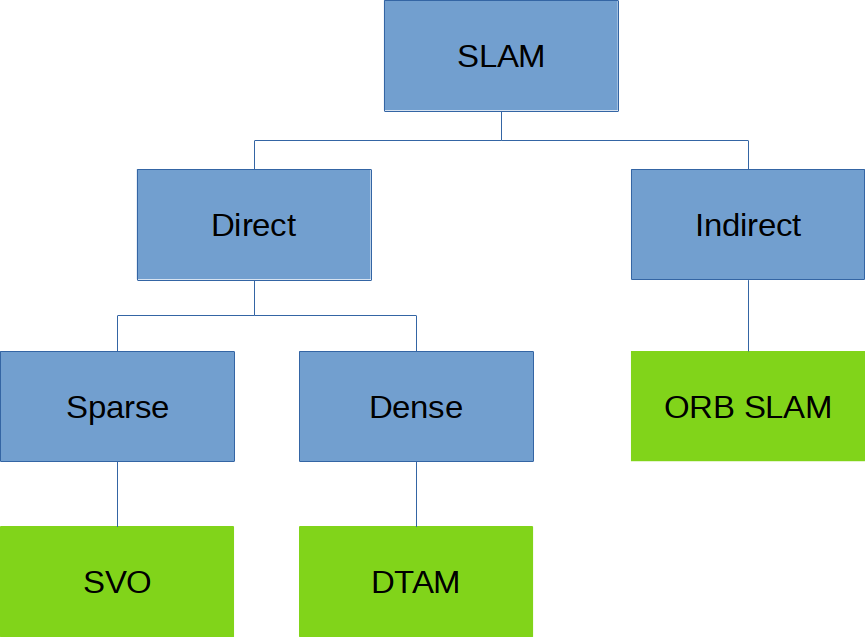
\includegraphics[width=1.0\textwidth]{img/slam_modes.png}
  \caption{SLAM Types}\label{fig:slammodes}
\end{figure}

As mentioned, we implement an SVO-like algorithm in this thesis. It is part of the direct sparse group.

\section{Stereo and Monocular SLAM}

In this thesis we focus on stereo SLAM. Many recent papers focus on monocular SLAM. The reason is that monocular cameras are cheaper and available on mobile phones. Monocular SLAM has two problems that do not prevail with stereo SLAM. First, an initialization process needs to estimate the pose and an initial point cloud over several images. It is not possible to calculate depth with only one image. Second, monocular SLAM cannot guess the scale of the point cloud. The intuition for this is that we can not distinguish between the movement of the camera on a small model close to the scene and the movement of the camera on the original model further away from the scene. With stereo SLAM we don not have this issue. For each camera pose we get two images with a known distance between the two camera sensors (baseline). Therefore, we can calculate the depth of points with a known scale. From this, we can generate 3D point clouds. We therefore have an instantaneous initialization and can calculate the pose in a known unit e.g. meters. Tracking between two camera poses is however the same for monocular and stereo SLAM.

\section{Camera}

To perform stereo computer vision, we need a stereo camera. There are a few stereo cameras available on the market. It is also possible to build a stereo camera with two monocular cameras. However, we decide against this option because it would require a mechanism to synchronize the images from both streams. We analyze three stereo cameras available on the market. An ideal camera would have a high frame rate, a high resolution, a global shutter, USB3.0 with UVC driver and a high baseline while being cheap. Table \ref{tab:cameras} shows a comparison of a ZED camera from Stereolabs \cite{zed}, a Tara from Econ \cite{tara} and a Realsense D435 from Intel \cite{realsense}.

\tiny
\begin{table}[H]
  \centering
  \begin{tabular}{|c|c|c|c|c|c|c|c|}
  Camera & Resolution & FPS & Shutter & Driver & Baseline & IMU & Price \\
  \hline
  ZED & 1920x1080 & 30 & rolling &  UVC & 120mm & 6DoF & 449\\
  Tara & 752x480& 60 & global &  UVC &  60mm & 6DoF & 149\\
  D435 & 1280x720& 90 & global & UVC &  50mm & 6DoF & 179\\
\end{tabular}
\caption{Tested Camera Types}
\label{tab:cameras}
\end{table}
\normalsize

\begin{figure}[H]
  \centering
  \subfloat[Stereolabs ZED]{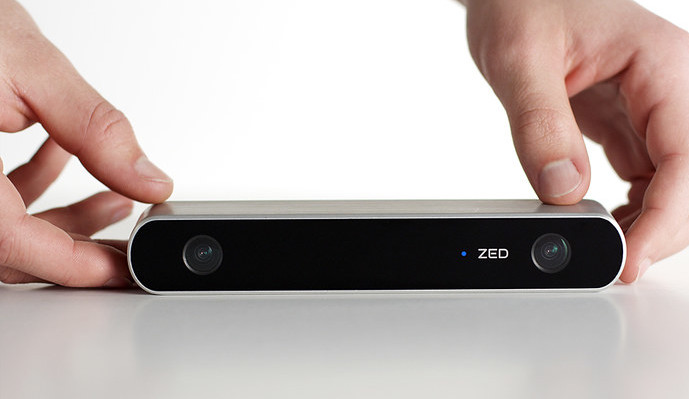
\includegraphics[width=0.3\textwidth]{img/zed_cam.jpg}}
  \subfloat[Econ Tara]{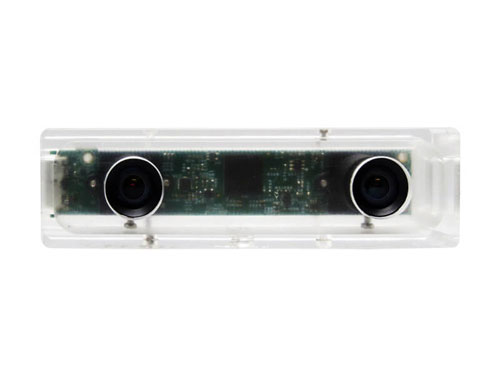
\includegraphics[width=0.3\textwidth]{img/tara_cam.jpg}}
  \subfloat[Intel Realsense D435]{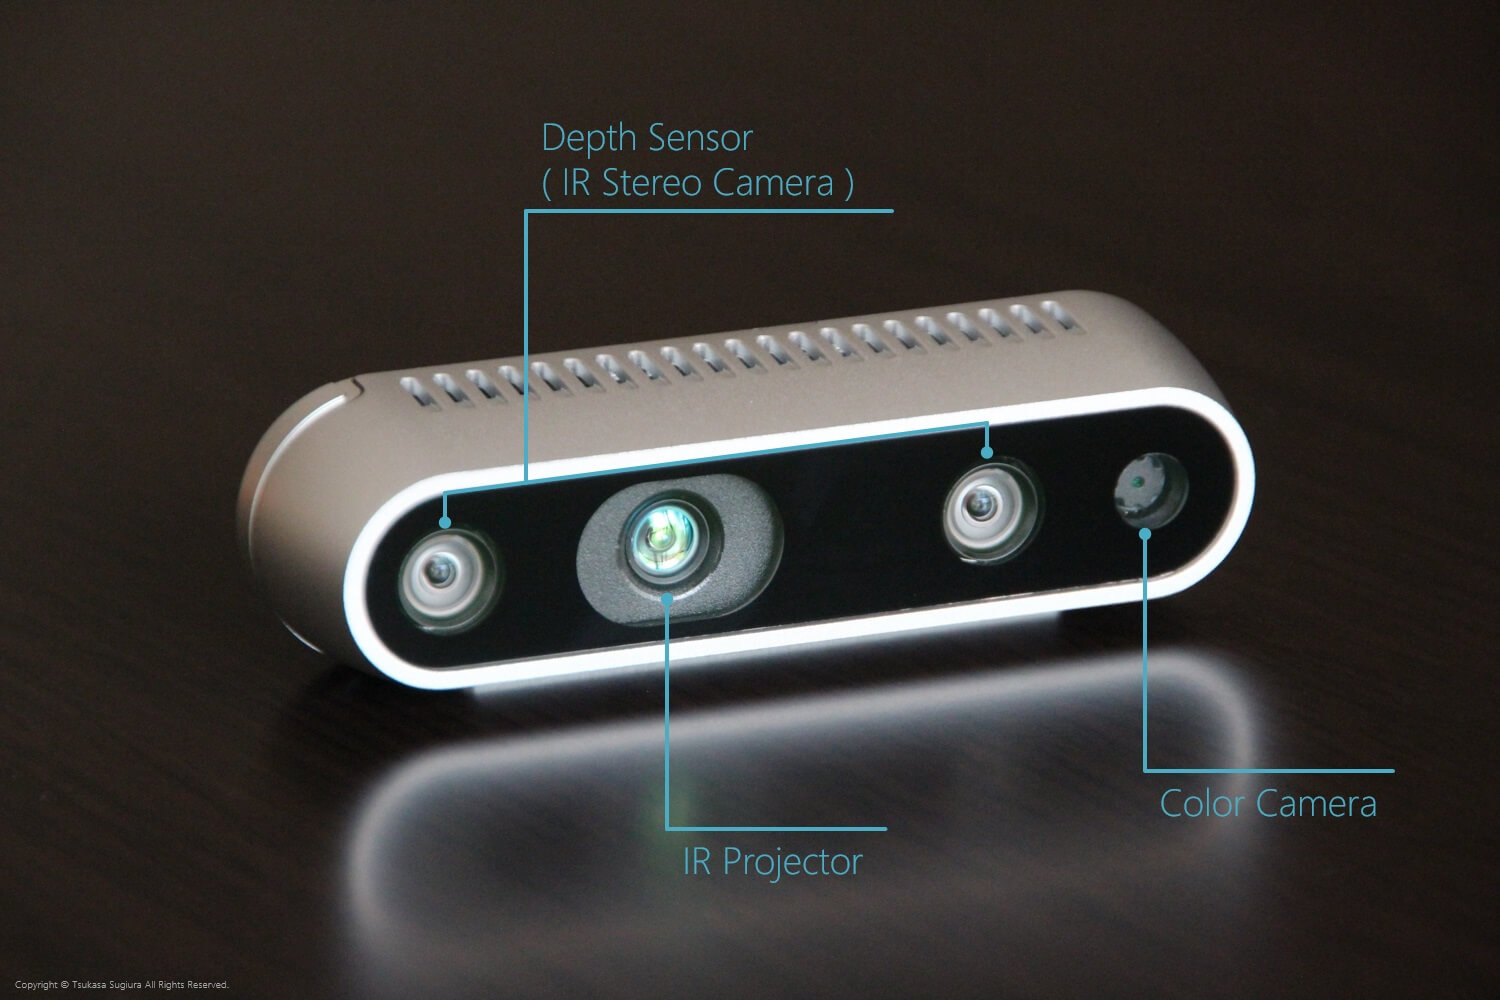
\includegraphics[width=0.3\textwidth]{img/d435_cam.jpg}}
  \caption{Tested Stereo Cameras}\label{fig:cameras}
\end{figure}


For this thesis we use the Econ Tara because it has an outstanding price ratio and because it is a conventional stereo camera.\\
The Intel RealSense camera can calculate depth images directly on the camera. For this thesis this is not wanted because we calculate the depth on our own.\\
The ZED camera has a huge baseline of 120mm. This allows depth estimation over higher range. We decide against this camera mainly because of the high price.

\section{Purpose of this Thesis}

This thesis implements SVO SLAM as an open source library. Based on this implementation we evaluate how well the algorithm is suited for embedded systems. We finally benchmark the implementation against the open source reference implementation, with regard to speed and accuracy. Furthermore, we provide a 3D viewer and a demo application showing the possibilities of the SLAM library.

\section{Outline}

This document is organised as follows. We describe the SVO algorithm in chapter \ref{ch:svo}. We keep the chapter succinct by providing the mathematical details in later chapters. Chapter \ref{ch:depth} describes how we receive depth information from a stereo camera. In chapter \ref{ch:opt_flow} we describe optical flow. We first start with an intuitive section and then move forward to the mathematical details. In chapter \ref{ch:pose_refinement} we present the mathematics about how to refine the pose after a first estimate. The implementation of the algorithm is subject of chapter \ref{ch:implementation}. We then compare the results of the implementation with previous work in chapter \ref{ch:results}. Ultimately, in chapter \ref{ch:discussion}, we discuss the final results.

\section{Planing}
The master thesis is honored with 27 ECTS. 1 ECTS consumes 30h which results in 810h. Assuming 8.5 working hours per day, we have to spend 95.29 working days. Because the thesis is done part time, we can use a full year. We assume one year has 48 weeks. During the first 16 weeks we can only spend 1.5 days for the thesis (because of additional modules). This means during the first 16 weeks we only work 24 days on the project. 71.29 days are left for the last 32 weeks. This results in 2.228 days work during the 32 weeks. Figure \ref{fig:gantt} shows the initial and the final planning.\\
Implementing the library took more time than expected. Therefore, plane detection and mesh creation has been removed. If this is required an additional library like the open source ``Point Cloud Library'' \cite{pcl} can be used.

\begin{figure}[H]
  \subfloat[Inital planing]{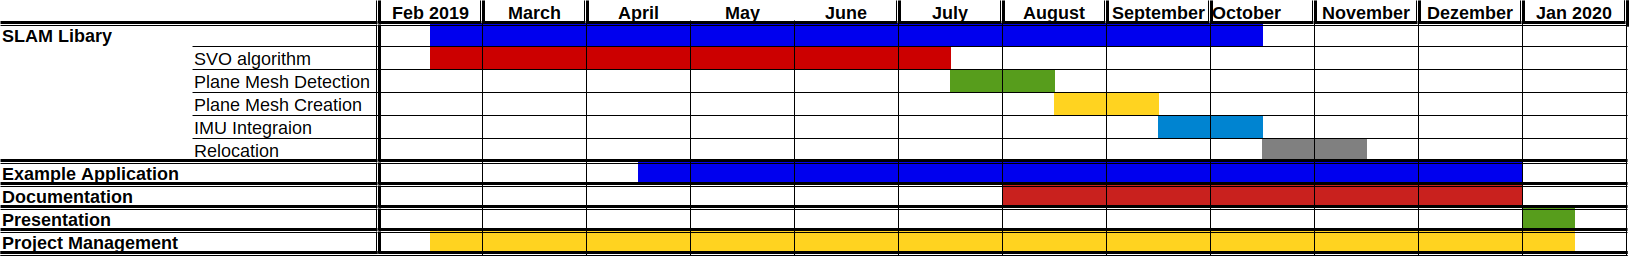
\includegraphics[width=1.0\textwidth]{img/gantt_orig.png}}\\
  \subfloat[Final planing]{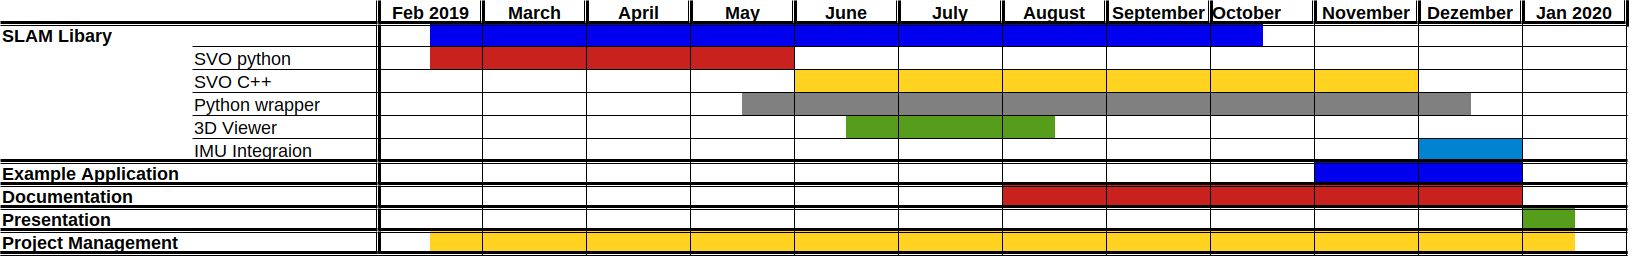
\includegraphics[width=1.0\textwidth]{img/gantt_final.png}}
  \caption{Planing}\label{fig:gantt}
\end{figure}

As the final planning shows we first started with a Python based implementation of the algorithm. The idea was that Python code is more readable and better suited for experimenting. However, the problem was that the code was slow even when using Numpy to speed up matrix multiplications. Therefore, we implemented the library completely in C++. However, for debugging a Python wrapper was developed in parallel. Reviewing this decision, this was a mistake because we spent a lot of time for debugging the Python wrapper. The final version still provides the wrapper. However, it is tested poorly and not documented.\\
Initially there was no plan to write a 3D viewer. However, to make it more flexible we developed a viewer which can receive data over network to keep the code base separated and to allow remote analysis of 3D data. Because of this two issues and changes we reduced the scope, and we set the focus on the library.

\chapter{SVO}\label{ch:svo}
The subject of this chapter is the basic idea behind SVO SLAM. We don't dive into the mathematical details yet. We will see that most parts of the algorithm are based on the idea of optical flow. Therefore, we will handle this topic in chapter \ref{ch:opt_flow}.

\section{Architecture}

Figure \ref{fig:svo_slam} shows the architecture of SVO compared to our implementation. It depicts many differences between the original implementation and what we do. However, the two main steps, which are sparse model based image alignment and pose refinement, are the same. Our implementation does not use multi-threading, such that everything is done sequential. This decision makes the duration to process one frame more deterministic. Because we focus on stereo cameras, we don't have to implement the mapping task in the same complexity as in the monocular implementation.

\begin{figure}[H]
  \centering
  \subfloat[Original SVO]{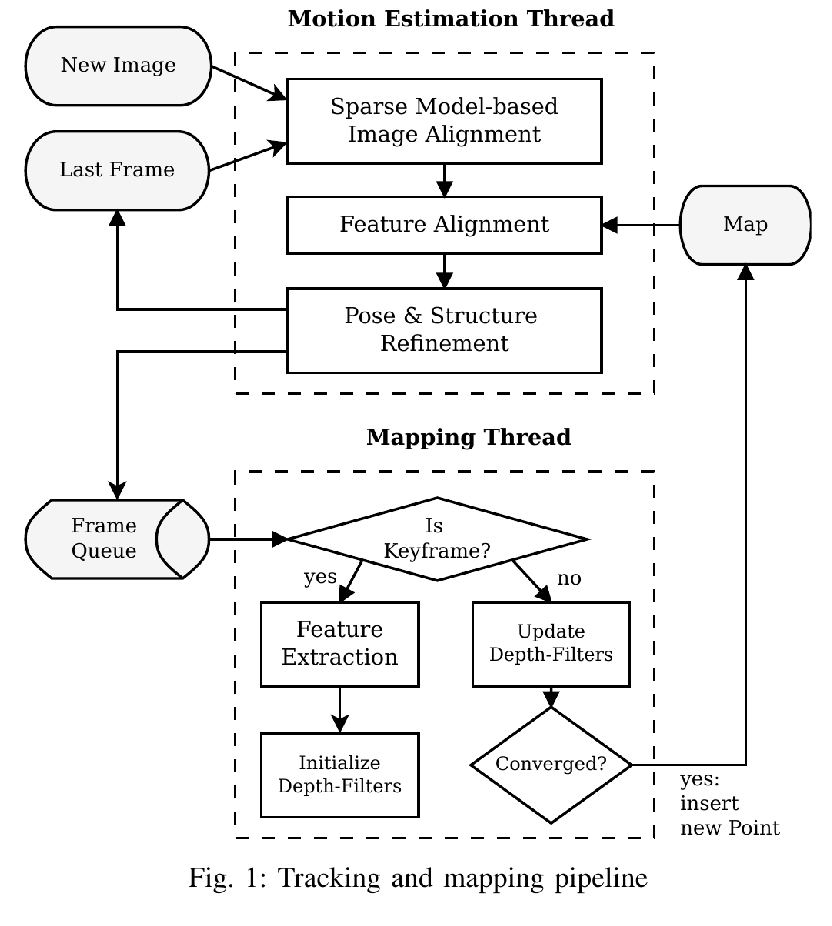
\includegraphics[height=0.25\textheight]{img/svo1_flow.png}}
  \qquad
  \subfloat[Our SVO]{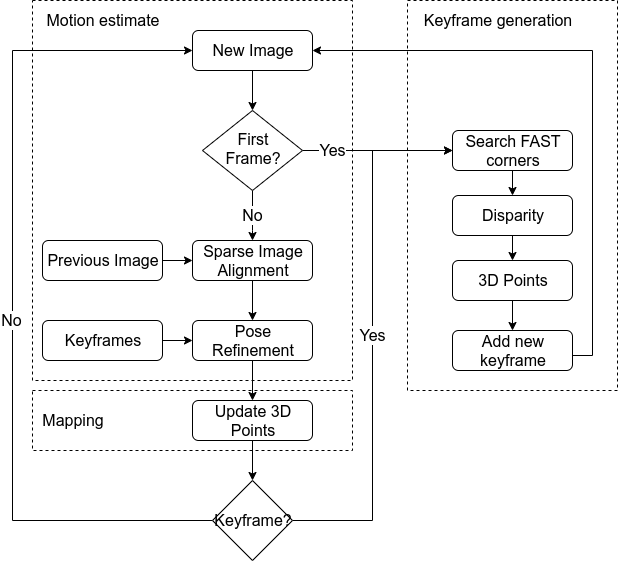
\includegraphics[height=0.25\textheight]{img/our_svo_slam.png}}
  \caption{Orignal SVO SLAM vs modified version}\label{fig:svo_slam}
\end{figure}

\section{Keyframe Generation}\label{sec:initialization}
The original SVO implementation uses a monocular camera. It is therefore not possible to estimate depth with the first image. In order to estimate the depth of keypoints, a movement along x or y axis is required. However, in this thesis we use a stereo camera with a known baseline. Therefore, we can estimate the depth of a keepoint from the first image. To generate a new keyframe, we perform the following steps:
\begin{enumerate}
  \item{Search FAST keypoints in the image \cite{fast}}
  \item{Do Sobel filtering of the image in horizontal direction}
  \item{Divide image in $n*m$ blocks}
  \item{Select one FAST corner in each block}
    \begin{enumerate}
      \item{If we can't find a FAST corner, we use the point with the biggest gradient from Sobel filtering as keypoint}
    \end{enumerate}
  \item{Reuse keypoints found in previous keyframes. Insert only new keypoints in empty blocks}
  \item{Calculate depth for each new keypoint}
  \item{Transform the keypoint depth to world coordinates by using the camera pose}
\end{enumerate}

Chapter \ref{ch:depth} shows the details on how we calculate the depth and the world coordinates from a stereo image.

\section{Sparse Image Alignment}\label{sec:sia}

\begin{figure}[H]
  \centering
  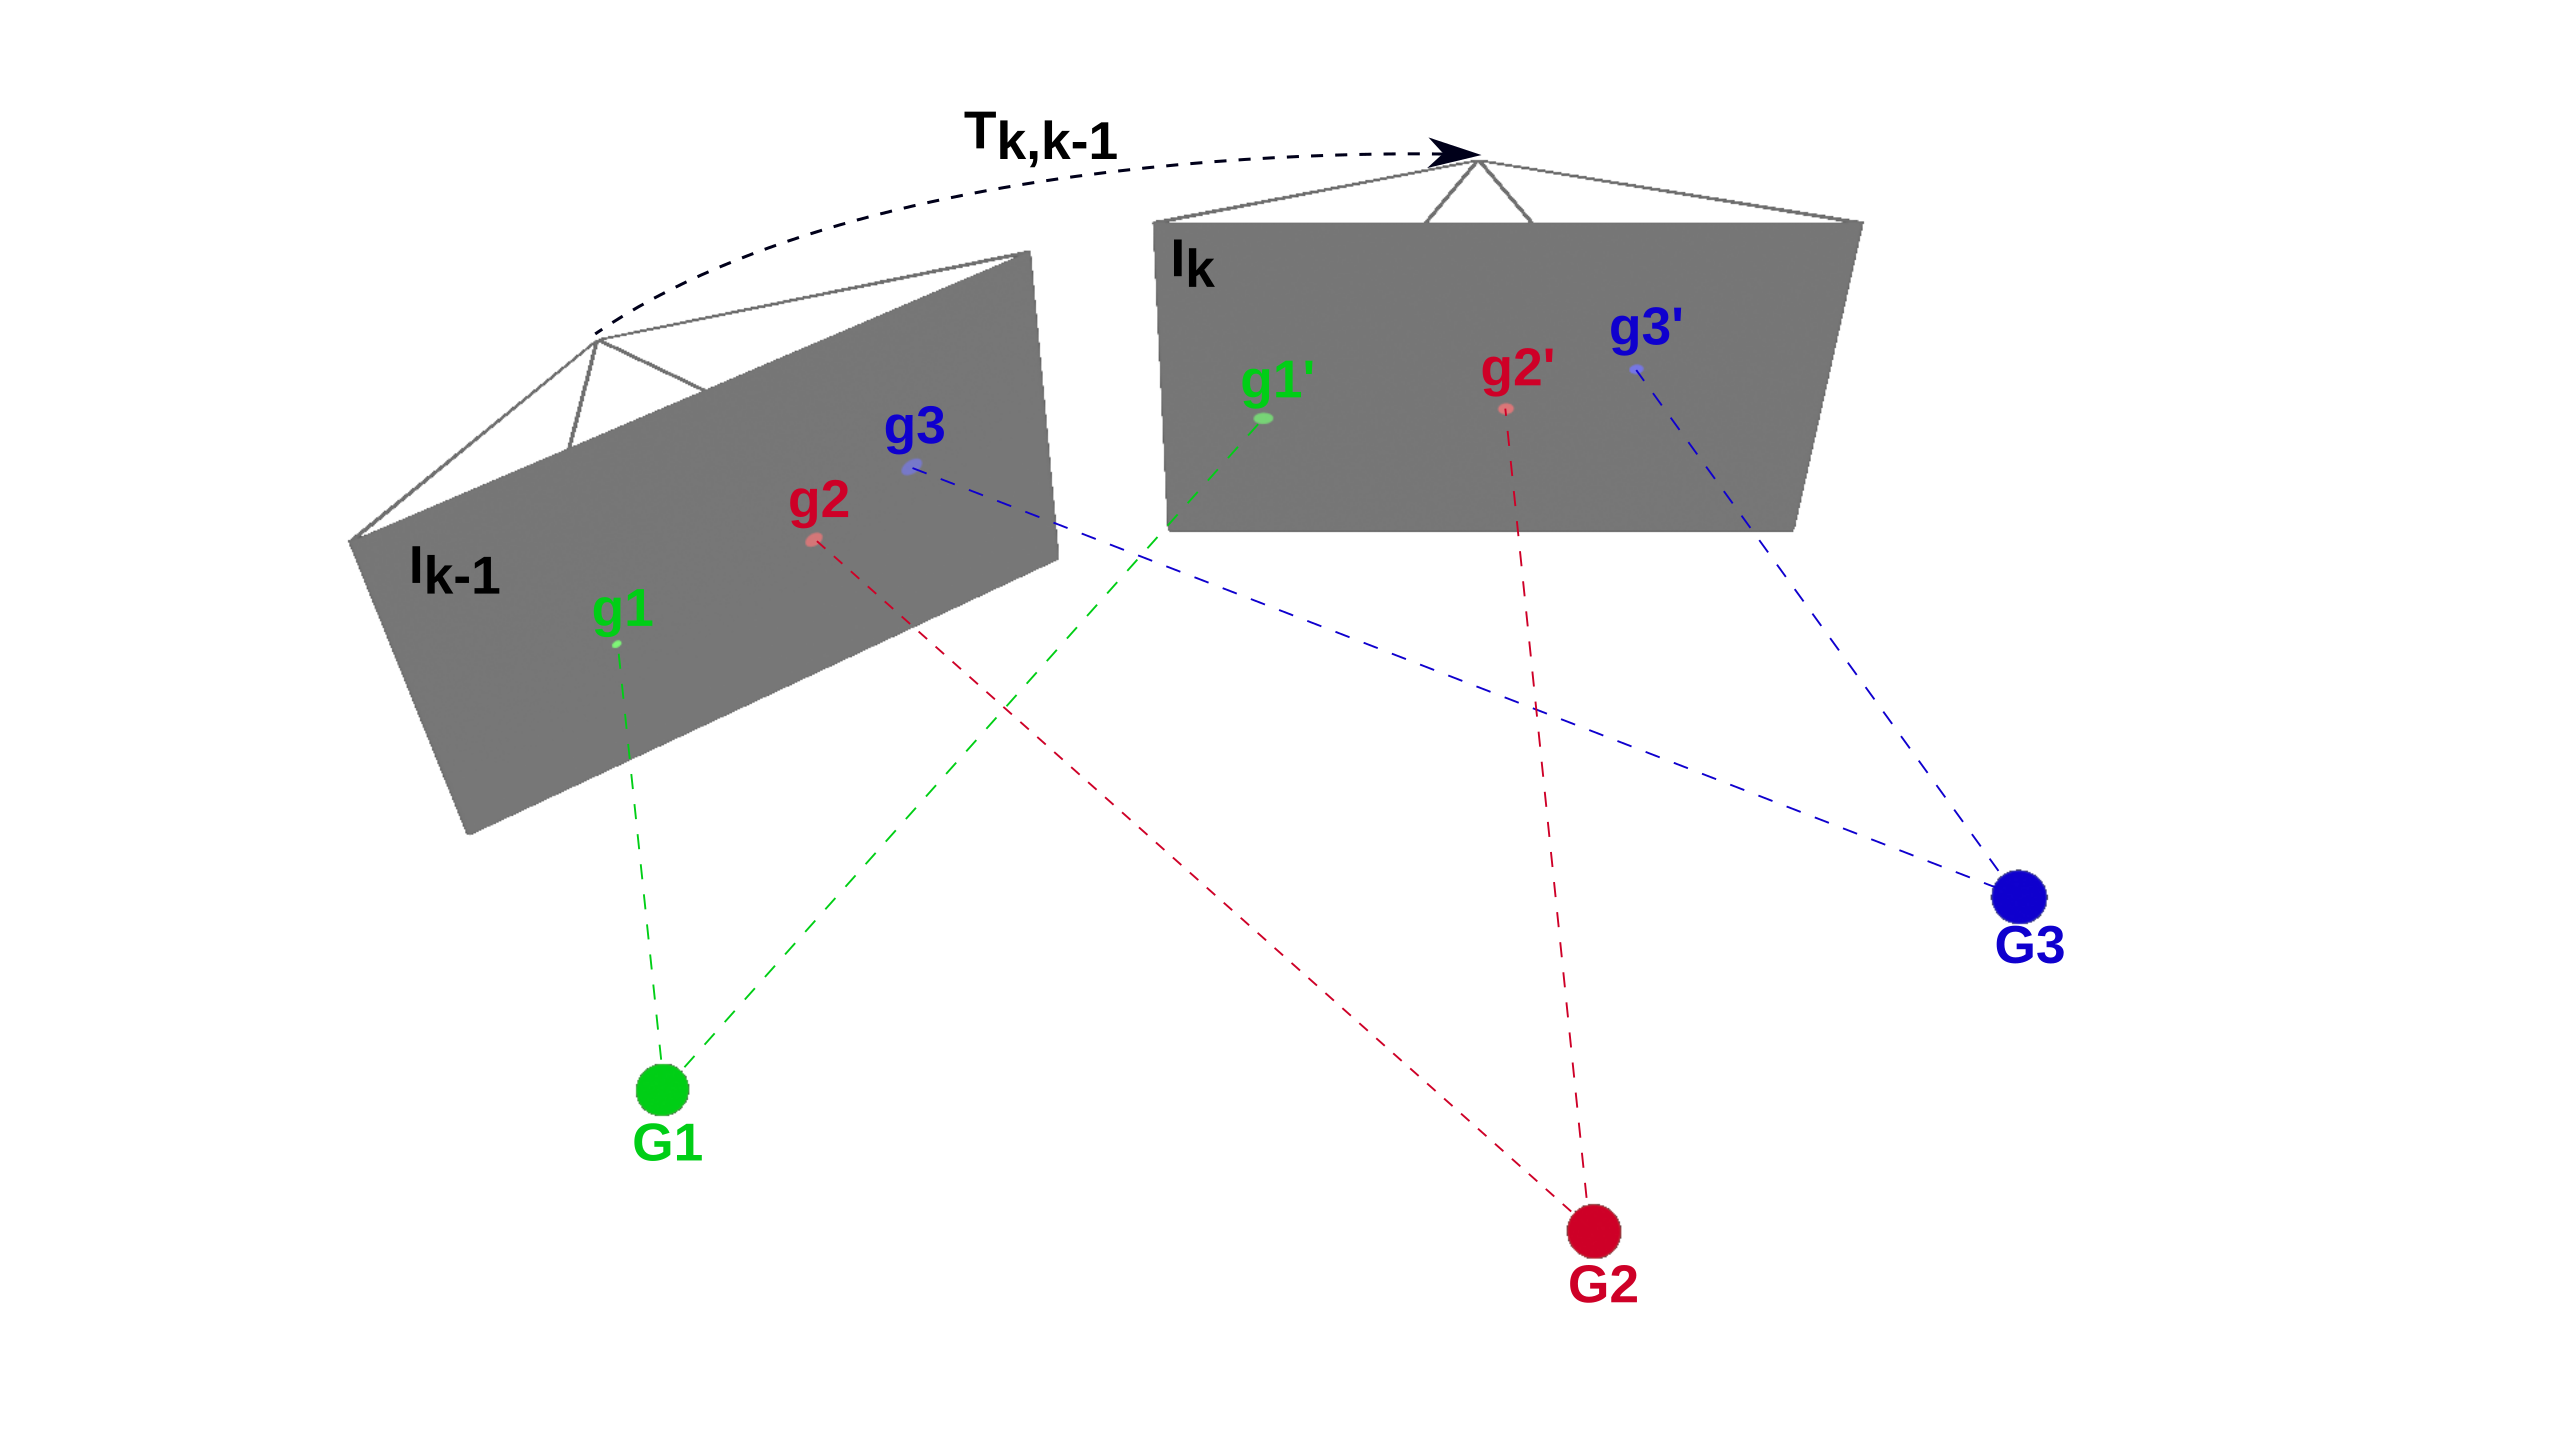
\includegraphics[width=0.99\textwidth]{img/pose_estimation_sparse.png}
  \caption{Sparse Image Alignment with previous frame $I_{k-1}$ and current frame $I_{k}$. Keypoint position g' by projecting G with $T_{k,k-1}$ to the image}
  \label{fig:sparse_image_alignment}
\end{figure}


From the keyframe generation step we get an initial point cloud. We use this point cloud to estimate the pose and motion of the camera. We try to find a pose that minimizes the photometric error of small patches around the keypoints. The photometric error is the intensity difference between two subsequent images. We do this by minimizing the formula shown in equation \ref{eq:intensity}. We use equation \ref{eq:camera_model} to project the 3D point cloud to the current frame. This step is shown in figure \ref{fig:sparse_image_alignment}. T corresponds to our extrinsic matrix written as rotation and translation matrix in equation \ref{eq:camera_model}. By using Gradient Descent we can minimize the intensity difference by changing the values of the extrinsic matrix $r_{ij}$ and $t_{x,y,z}$. As an initial guess for the pose we use the current pose and add the motion model. The motion model is the difference between the pose in the previous frame $t-1$ and frame $t-2$. If we have an additional IMU available, we can also improve the motion model by adding information from this sensor (e.g. angle velocity from gyroscope).

\begin{equation}\label{eq:camera_model}
  \begin{gathered}
    \begin{pmatrix}
      u\\
      v\\
      s
    \end{pmatrix}=
    \begin{pmatrix}
      f_x & 0 & c_x \\
      0 & f_y & c_y \\
      0 & 0 & 1
    \end{pmatrix}
    \begin{pmatrix}
      r_{11} & r_{12} & r_{13} & t_x\\
      r_{21} & r_{22} & r_{23} & t_y\\
      r_{31} & r_{32} & r_{33} & t_z\\
    \end{pmatrix}
    \begin{pmatrix}
      X\\
      Y\\
      Z\\
      1
    \end{pmatrix}\\
    \begin{pmatrix}
      x\\
      y
    \end{pmatrix}=
    \begin{pmatrix}
      \frac{u}{s}\\
      \frac{v}{s}
    \end{pmatrix}\\
    =>g=h(CTG)=h(PG)
  \end{gathered}
\end{equation}
\begin{align*}
  f_x,f_y  &:  \text{Focal length}\\
  c_x,c_y  &:  \text{Principal point (z axis of camera goes through)}\\
  X,Y,Z     &: \text{Point coordinates with local camera coordinates}\\
  u,v,s     &: \text{Image coordinates with scale s}\\
  x,y       &: \text{Keypoint projection from 3D cloud}\\
  r_{ij}    &: \text{Camera rotation parameter}\\
  t_{x,y,z} &: \text{Camera translation}\\
  g         &: \text{2D point x,y}\\
  G         &: \text{3D point X,Y,Z}\\
  C         &: \text{Intrinsic Camera Matrix}\\
  T         &: \text{Extrinsic Camera Matrix (Pose)}\\
  h         &: \text{Camera coordinates (u,v,s) to pixel coordinate (x,y) function}\\
  P         &: \text{Projection Matrix}
\end{align*}

\begin{equation}\label{eq:intensity}
  \sum_{a \in A}\sum_{x=a_x-\frac{m}{2}}^m\sum_{y=a_y-\frac{n}{2}}^n(I_{k-1}(x'',y'')-I_{k}(x',y'))^2
\end{equation}
\begin{align*}
  m,n         &: \text{Patch size}\\
  x'',y''    &: \text{Warped pixel position in the template}\\
  x',y'      &: \text{Pixel position in the current image}\\
  I_{k-1}    &: \text{Template image}\\
  I_{k}      &: \text{Current image}\\
  A          &: \text{For all keypoints}
\end{align*}

The SVO paper \cite{svo} describes this step in section IV.A. By performing the sparse image alignment, we get a first estimate of the pose. However, because we estimate the current pose by using the previous frame we get a drift in the long term. Therefore, we need to refine the pose by using the keyframes as reference. This is what we describe in the next section. Section \ref{sec:pose_estimation} will describe the optimization in more detail.

\section{Pose Refinement}\label{sec:refinement}
\begin{figure}[H]
  \centering
  \subfloat[Optical Flow with keyframes $I_{r1,2}$. New keypoint position g' found with optical flow]{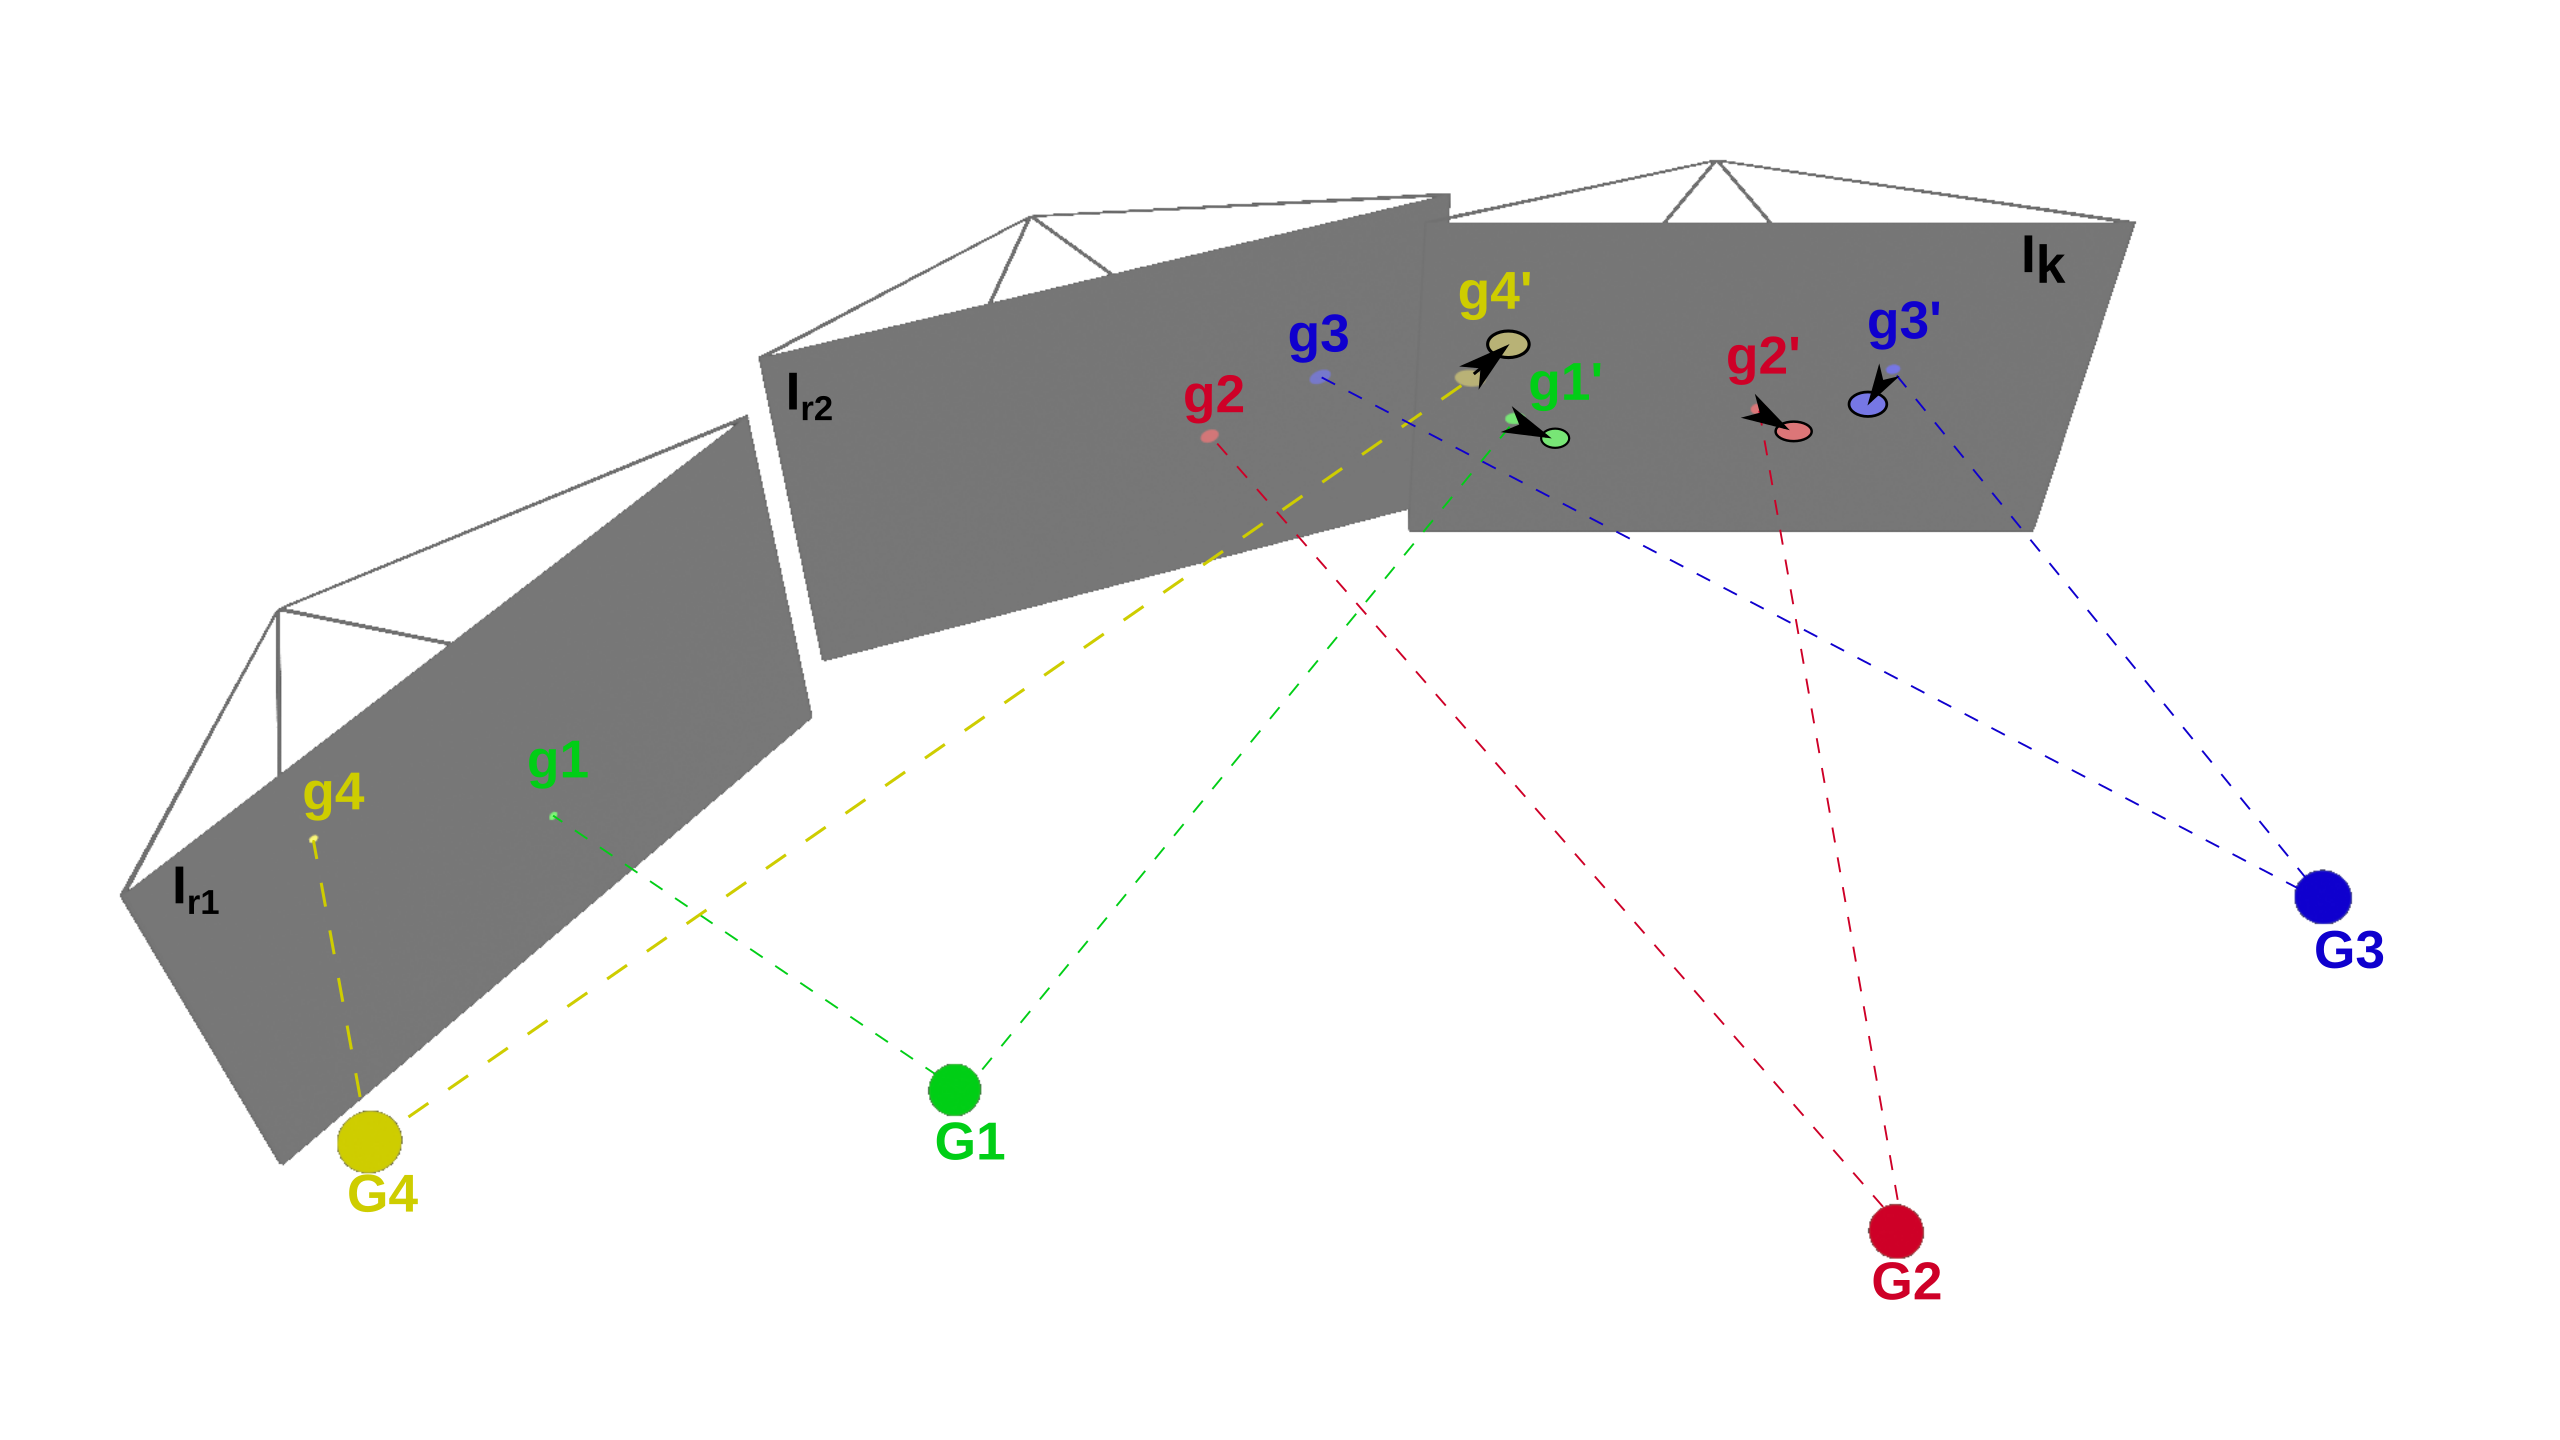
\includegraphics[width=0.99\textwidth]{img/pose_estimation_opt_flow.png}}\\
  \subfloat[Pose $T_R$ refinement based on difference between keypoint position from sparse image alignemnt and optical flow]{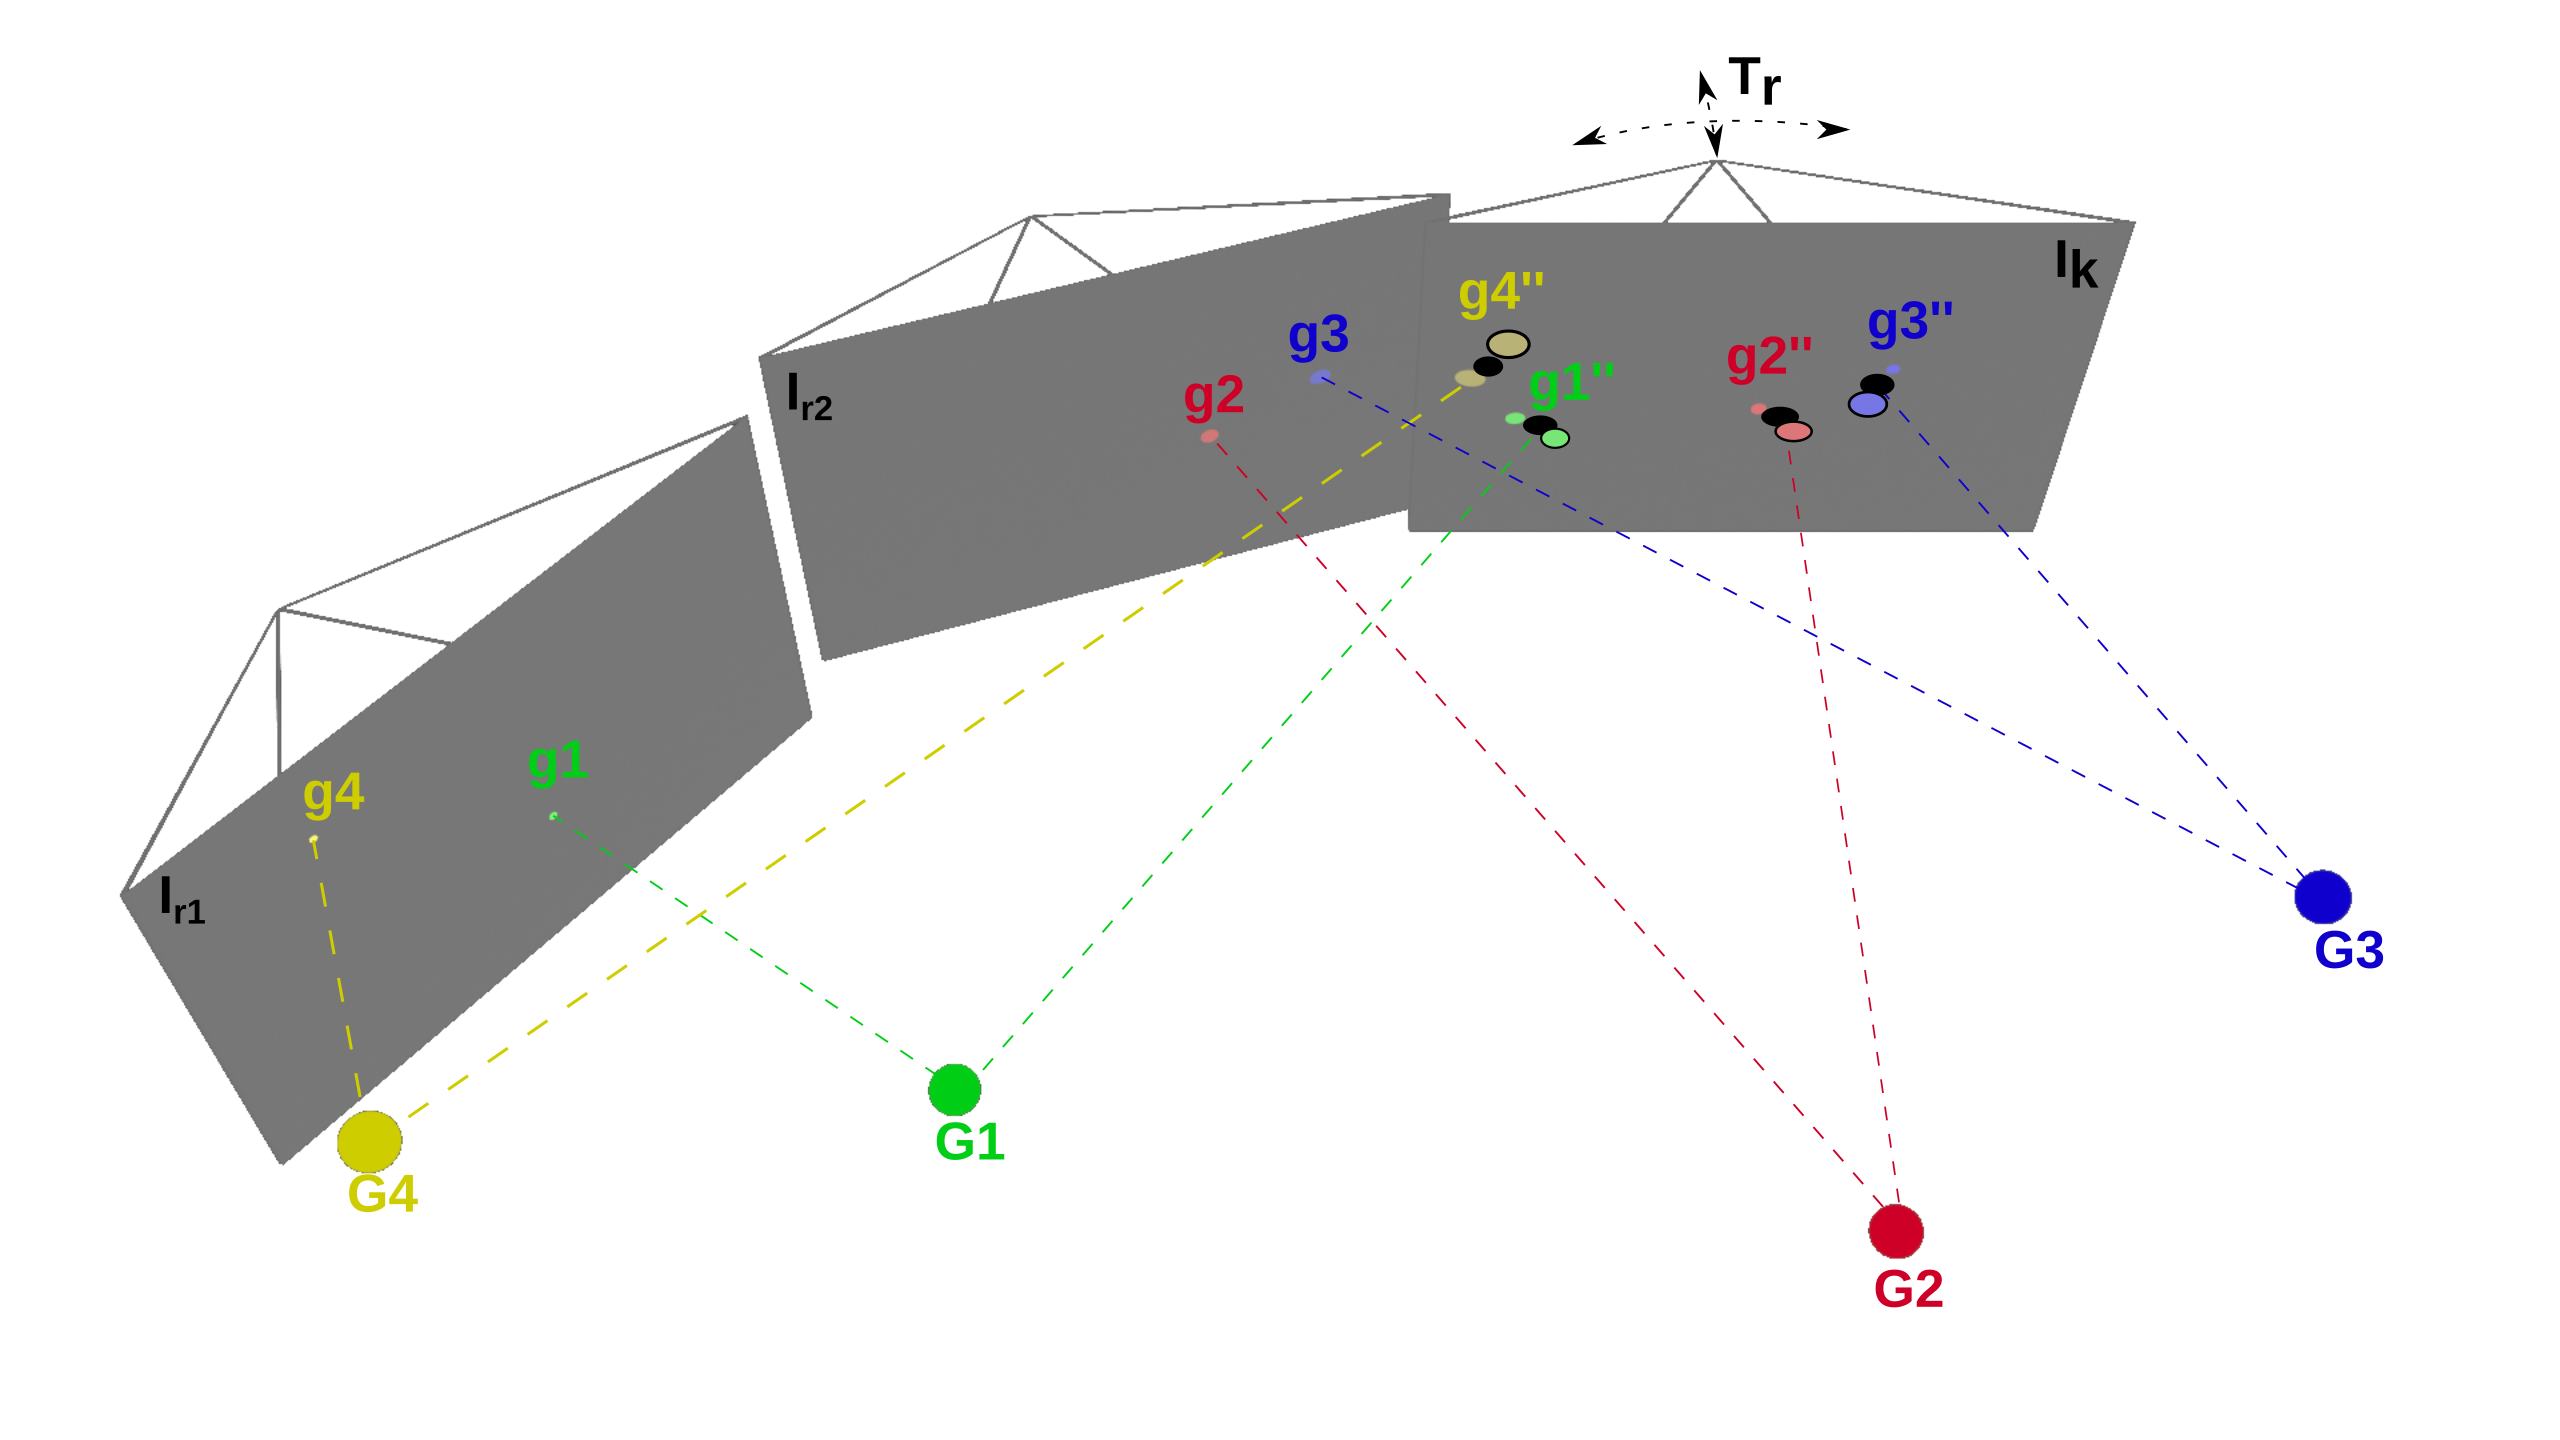
\includegraphics[width=0.99\textwidth]{img/pose_estimation_refinement.png}}
  \caption{Pose Refinement}\label{fig:pose_refinement}
\end{figure}

The refinement step is necessary to reduce the drift over time by using the keyframe where we first saw the keypoint. We use the Inverse Compositional Lucas Kanade algorithm to find an updated position of the point in the current image. We show this step in figure \ref{fig:pose_refinement}a. By using the pose from sparse image alignment we get an estimate of the 2D point position in the current image. After that we use optical flow to get a more accurate 2D point position. Afterwards we start to optimize the pose by minimizing the re-projection error shown in equation \ref{eq:refinement_problem}. We show this process in figure \ref{fig:pose_refinement}b.

\begin{equation}\label{eq:refinement_problem}
  \begin{gathered}
    \min_P(\sum_{a \in A|x'=a_x,y'=a_y}((x'-x(P))^2+(y'-y(P))^2))\\
  \end{gathered}
\end{equation}
\begin{align*}
  x',y'   &: \text{2D Point position found by optical flow}\\
  x,y     &: \text{2D Point projected from 3D (see \ref{eq:camera_model})}\\
  P       &: \text{Projection matrix}\\
  A       &: \text{For all keypoints}\\
\end{align*}

Chapter \ref{ch:opt_flow} describes optical flow and Lucas Kanade in more details. Chapter \ref{ch:pose_refinement} describes how we calculate the gradient for minimizing the re-projection error in equation \ref{eq:refinement_problem}.

\section{Keyframe Insertion}
In every frame we should see one keypoint for each grid. Because some keypoints are weak or do not project to the current frame, we normally have less keypoints available for pose estimation. If the number drops below 66\% of the theoretic count, we insert a new keyframe. The process for adding a new keyframes is described in section \ref{sec:initialization}.

\section{Update 3D Points}\label{sec:point_update}

The update of 3D points is different from what SVO \cite{svo} describes. The reason is again that we can measure the keypoint depth in the first frame by using the stereo image. SVO uses a bayesian filter approach \cite{svo} to estimate the keypoint depth over time. We instead use a mechanism to detect outliers and a simple Kalman Filter to update the 3D position of 3D keypoints.

\subsection{Outlier Detection}
We base outlier detection on two steps. First, we check the intensity difference returned by optical flow during pose refinement. If it exceeds a value of 20 which was found empirically, it will drop the point from the list of usable points. This can happen if points get occluded by objects and are therefore not visible in the new image anymore. Another mechanism that doesn't mark a point as outlier but masks it during refinement is if a point moves more than 9pixels. This happens for points in areas with low texture. We don't use such points during refinement. However, such points can still help to improve the position during sparse image alignment.\\
We use a second mechanism to detect outliers after pose refinement. We use the stereo image and calculate the disparity for a keypoint $d_{current}$. We then transfer the global 3D keypoint to local coordinates. By calculating $d_{expected}=z_{local}/baseline$ we get the expected disparity. We consider the estimate as inlier if the difference is smaller than 2.5 pixel $abs(d_{current}-d_{expected})<2.5$. We take the standard deviation of 0.5 pixel for disparity and want to include 99.99\% which corresponds to 5 Tau. If a point has more outlier than inlier, we remove it from the keypoints. This mechanism eliminates weak keypoints with low contrast.

\subsection{Point Refinement}
\begin{figure}[H]
  \centering
  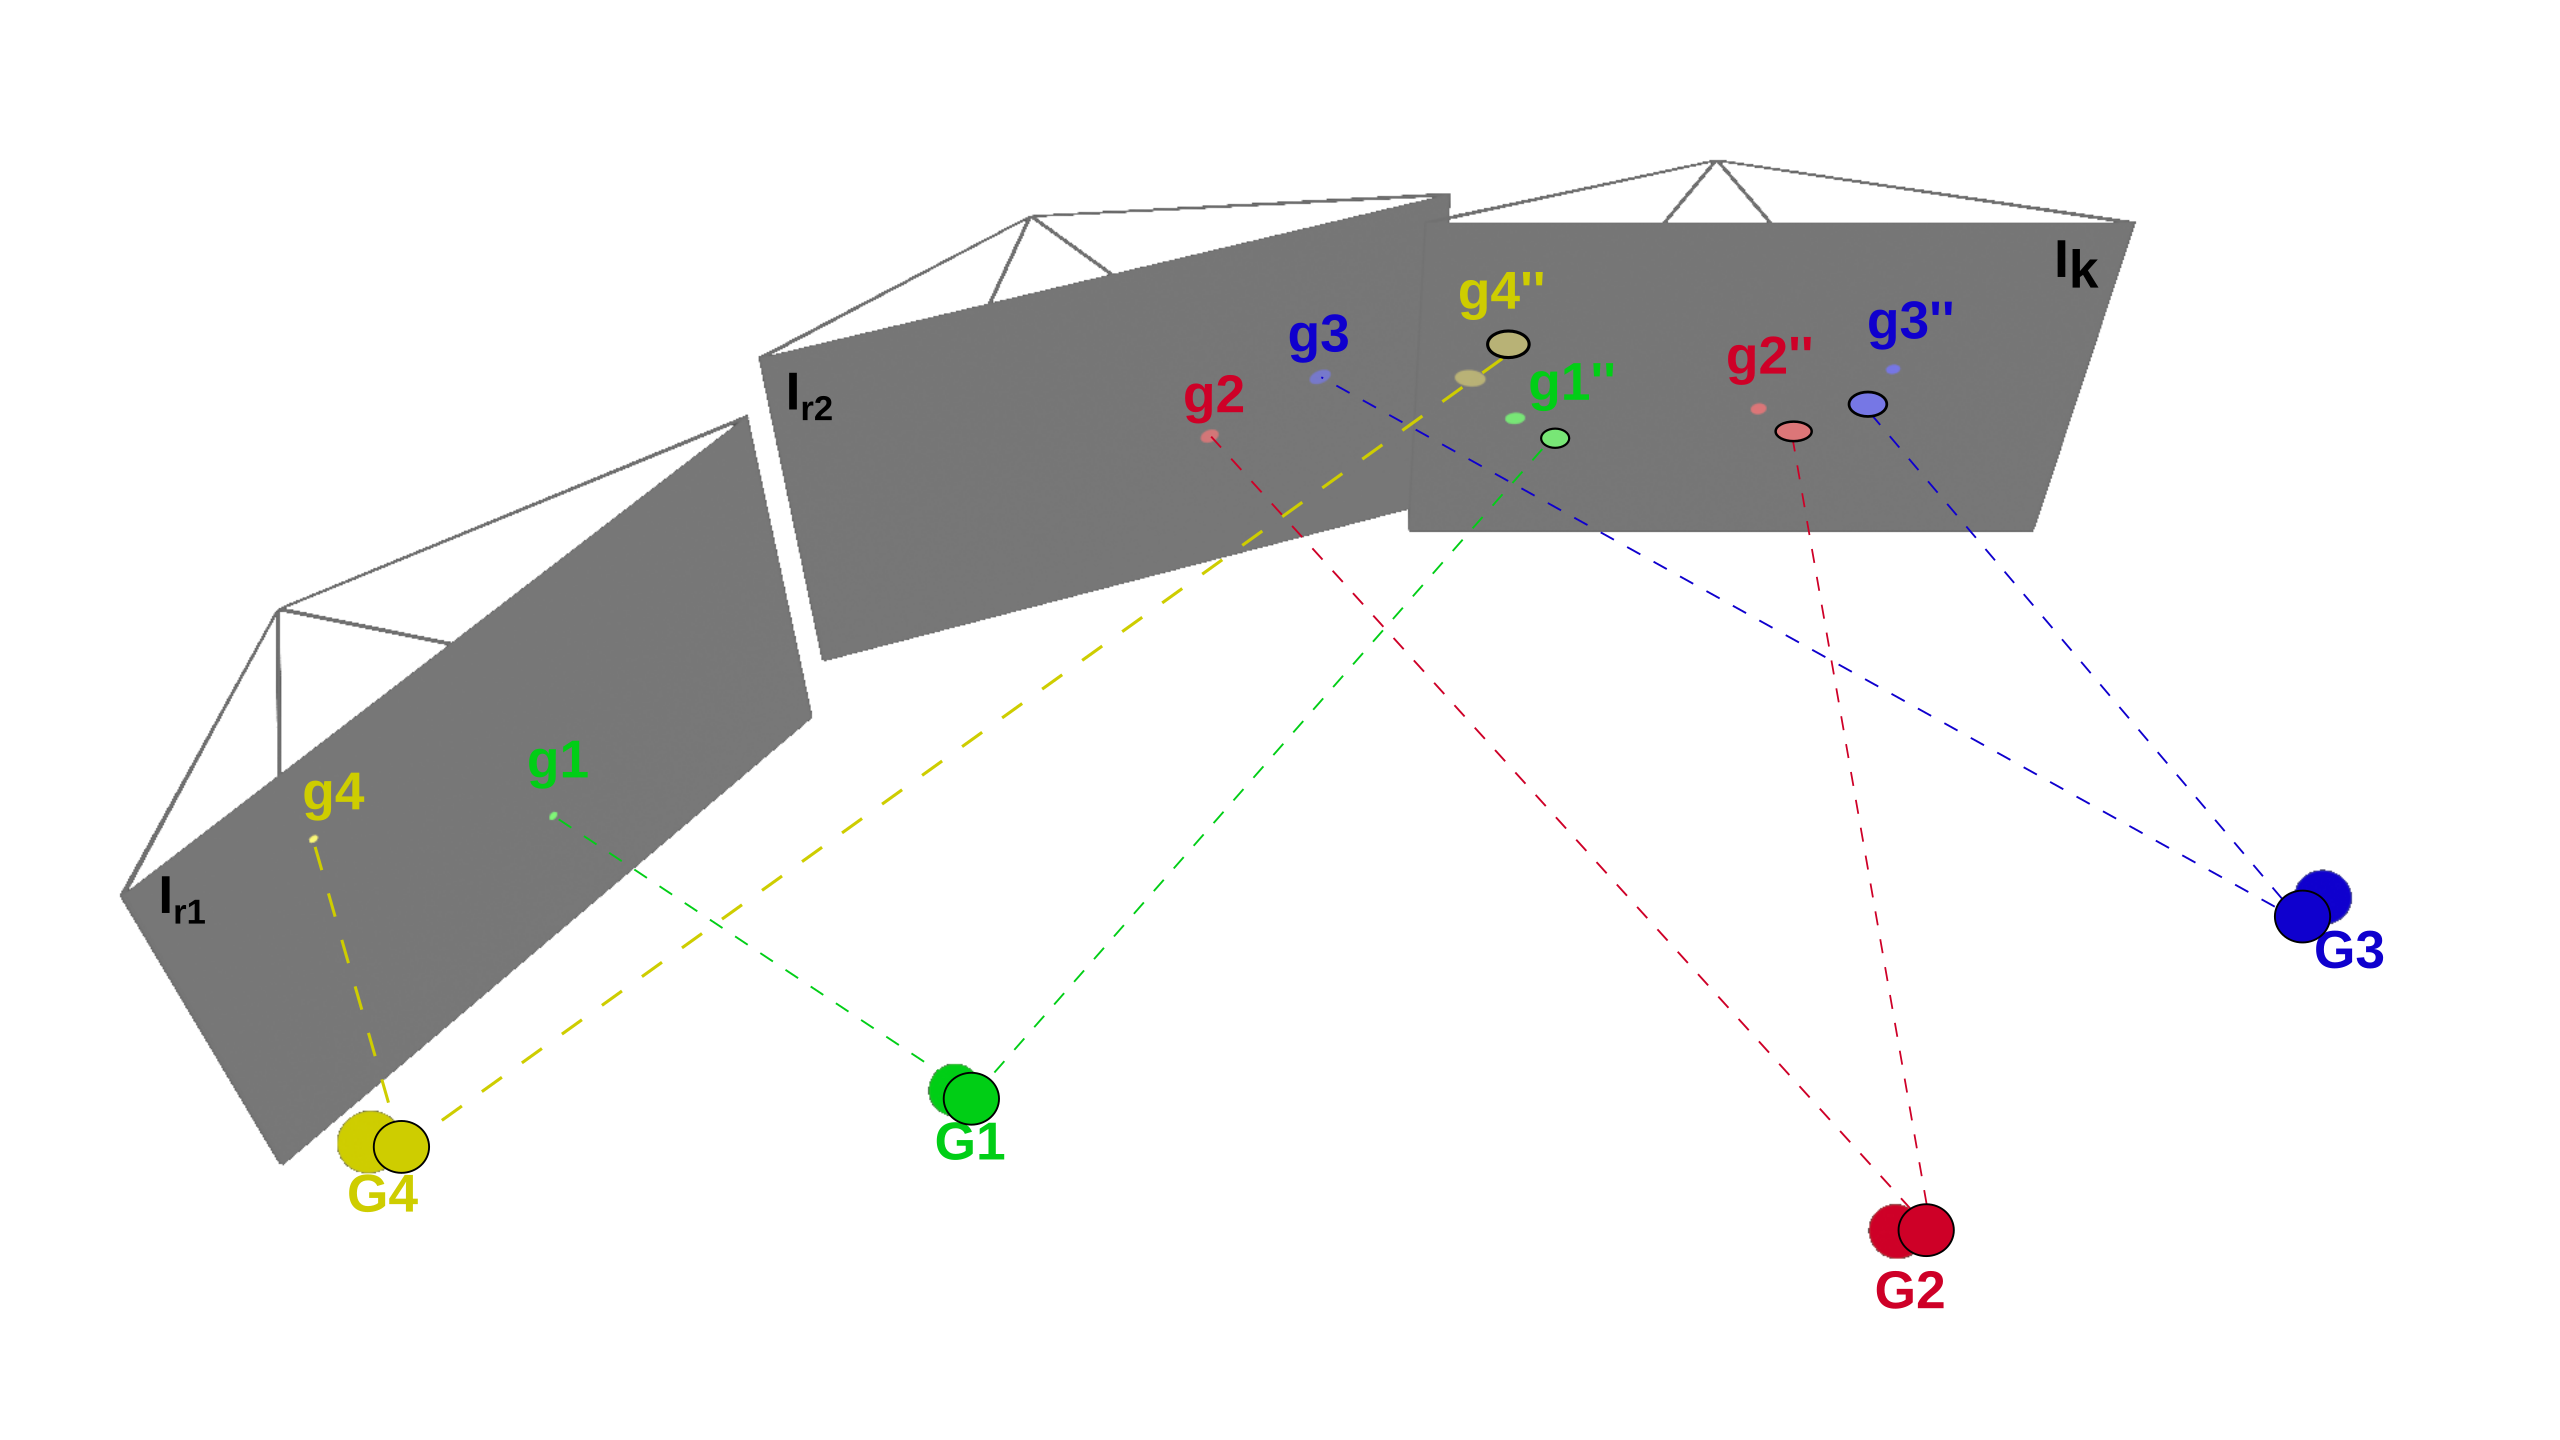
\includegraphics[width=0.99\textwidth]{img/pose_estimation_point_update.png}
  \caption{3D Point Refinement based on 2D point position from optical flow}
  \label{fig:point_update}
\end{figure}

In section \ref{sec:refinement} we refined the keypoint position in the image with optical flow. We then refined the pose by minimizing the re-projection error. If we use the refined pose to project the points to the image we still have a small error between this points and the points from optical flow. This comes because of some inaccuracy in the depth estimation. We use movements of the camera, that are bigger than the baseline of the camera, to improve the accuracy of the 3D point cloud (figure \ref{fig:point_update}). We update the 3D points by using a Kalman filter with an update and state equation shown in \ref{eq:point_refinement}. We use the same definitions for the Kalman Filter as \cite{statdig}. The error of our new depth estimate is smaller the bigger the movement is. For the first measurement we know that the movement has the length of the baseline of the camera. This means that instead of $\sqrt{\Delta x^2+\Delta y^2}$ we just use the baseline in meter. The disparity has a close to normal distribution with a standard deviation of 0.5 pixel. Therefore, we use the inverse depth to update our Kalman filter. Therefore we update $z^{-1}$ and not $z$. The standard deviation of 0.5 pixel is because we have a maximum resolution for disparity of one pixel. The variance for new information $w$ should be a small number close to zero.
\begin{equation}\label{eq:point_refinement}
  \begin{gathered}
    z^{-1}(t)=z^{-1}(t-1)+w(t)\\
    y(t)=z^{-1}(t)+v(t)\\
    w(t)=0.001\\
    v(t)=(\frac{0.5}{\sqrt{\Delta x^2 + \Delta y^2}})^2\\
  \end{gathered}
\end{equation}
\begin{align*}
  \Delta x, \Delta y  &: \text{Movement of the camera}\\
  w                   &: \text{New information}\\
  v                   &: \text{Measurement error/noise}\\
\end{align*}

\chapter{Depth Estimation}\label{ch:depth}

To find the depth at a certain point (x,y) we match the intensities of the left and right images based on a patch of pixels (e.g. a square of 31x31 pixel) \cite{rvc}. The algorithm matches the right image at position (x,y) to the left image at the same position. Because we know the stereo camera is vertically aligned, it then increases x for the right image and matches again. We repeat this step up to the maximum allowed disparity (e.g. 50 pixels). The position with the smallest intensity difference between left and right is what we call disparity. An object far away has less disparity than an object close to the camera. This is what we show in figure \ref{fig:disparity}. We use an empiric patch size of 31x31 pixel for the Econ Tara at 752x480.

\begin{figure}[H]
  \begin{center}
    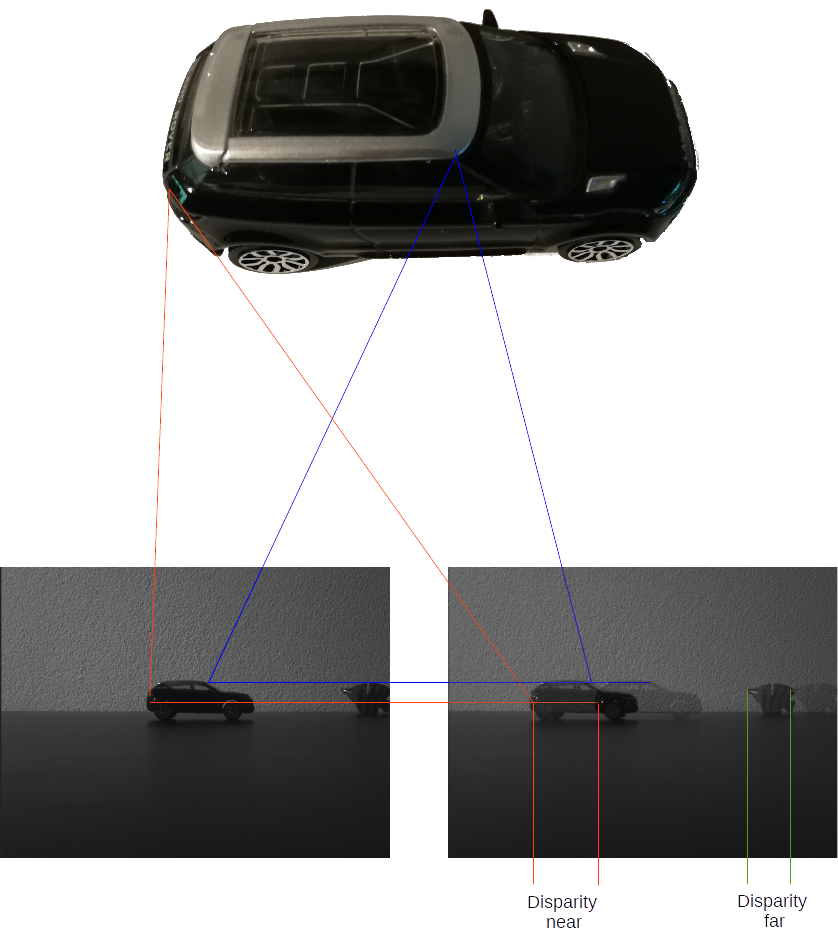
\includegraphics[width=0.9\textwidth]{img/disparity_concept.png}
  \end{center}
  \caption{Disparity with epipolar (horizontal) line, left: left image, right: right image with transparent left image}\label{fig:disparity}
\end{figure}

From disparity we can calculate the depth by using equation \ref{eq:depth_disp}.

\begin{equation}\label{eq:depth_disp}
  Z=\frac{f_m*b}{s_{px}*d}=\frac{f_x*b}{d}
\end{equation}
\begin{align*}
  Z        &: \text{Depth/Distance from camera}\\
  f_x      &: \text{Focal length in pixel}\\
  d        &: \text{Disparity}\\
  b        &: \text{Baseline in meter}\\
  f_m      &: \text{Focal length in meter}\\
  s_{px}  &: \text{Pixel size in meter}
\end{align*}

If we know the pose of the camera we can transform the depth to the global coordinate system. First we need to calculate the X and Y position in local camera coordinates. We show this in equation \ref{eq:depth_xy}.

\begin{equation}\label{eq:depth_xy}
  \begin{gathered}
    X = \frac{x-c_x}{f_x*Z}\\
    Y = \frac{y-c_y}{f_y*Z}\\
  \end{gathered}
\end{equation}
\begin{align*}
  X,Y,Z    &: \text{Point coordinates with local camera coordinates}\\
  f_x,f_y  &: \text{Focal length in pixel}\\
  c_x,c_y  &: \text{Image center (where z axis goes through)}\\
  x,y      &: \text{2D point in image}
\end{align*}

Now we can transform the 3D point from the cameras local coordinate system to the global coordinate system by using the camera pose. We show this in equation \ref{eq:depth_global}. Note that we set camera pose = extrinsic camera matrix. This can be different in other documents and implementations.

\begin{equation}\label{eq:depth_global}
  \begin{pmatrix}
    X'\\
    Y'\\
    Z'
  \end{pmatrix}=
  \begin{pmatrix}
    r_{11} & r_{12} & r_{13}\\
    r_{21} & r_{22} & r_{23}\\
    r_{31} & r_{32} & r_{33}\\
  \end{pmatrix}^{-1}
  \left(
  \begin{pmatrix}
    X\\
    Y\\
    Z
  \end{pmatrix}
  -\begin{pmatrix}
    t_x\\
    t_y\\
    t_z
  \end{pmatrix}
  \right)
\end{equation}
\begin{align*}
  X,Y,Z     &: \text{Point coordinates with local camera coordinates}\\
  X',Y',Z'  &: \text{Global point coordinates}\\
  r_{ij}    &: \text{Camera rotation parameter}\\
  t_{x,y,z} &: \text{Camera transition}
\end{align*}

We use this coordinates to create and maintain our point cloud.

\chapter{Optical Flow}\label{ch:opt_flow}

In this chapter we describe Lucas Kanade Optical Flow in more detail. This algorithm tries to find the movement of one or several points from one image to another. Lets assume we have an image I1 at time t-1 and an image I2 at time t. We know the position of a point P1 in image 1. We use Lucas Kanade Optical Flow to find the position P2 of the point in image 2. Figure \ref{fig:optical_flow} shows the problem we want to solve. We call the position change of the point optical flow.

\begin{figure}[H]
  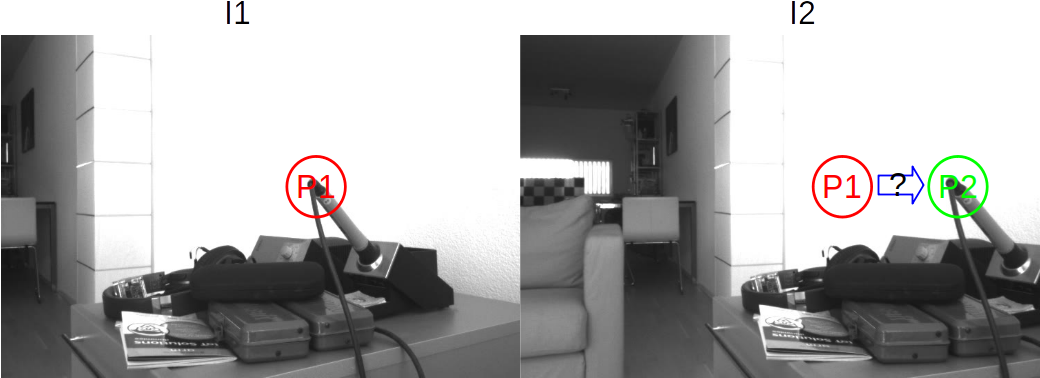
\includegraphics[width=1.0\textwidth]{img/optical_flow.png}
  \caption{Optical Flow: Where did the point at position P1 in image I1 move in image I2?}\label{fig:optical_flow}
\end{figure}

We divide this chapter into four sections. The first section describes Lucas Kanade in an intuitive but oversimplified way. Section two describes the original Lucas Kanade algorithm while section three focuses on the Inverse Compositional Lucas Kanade algorithm. In the last section we see an extension to guess a 3D pose. We use this method in the sparse image alignment step.

\section{Lucas Kanade Intuitive}

Lucas Kanade Optical Flow tries to identify where a point moves between two images as shown in figure \ref{fig:optical_flow}. It does that efficiently by using intensity gradients. This section describes how this works in an intuitive but simplified way while the next section describes it mathematically. In this section, we use the term intensity gradient for gradients that are defined by a Sobel filter and we call the gradient pointing towards the direction of movement ``position gradient''.\\
Let's assume the simplest scenario where we can only move in one direction (left or right). Figure \ref{fig:optical_flow_intuitive} shows this simple scenario. Let's first focus on the case where we have a small movement \ref{fig:optical_flow_intuitive}a. We calculate the intensity gradients in the template for a small patch of 3x4 pixel (first row). Then we calculate the intensity difference (last row) between the current image (second row) and the first image. Now we multiply the intensity gradient by the intensity difference, which will give us the direction in which we have to move (position gradient). Here we assume that moving the current patch to left means - and moving it to right +. Now we move in the positions gradient direction and will calculate the intensity difference again. If it increases, we moved too much and we have to reduce the step size if it decreases we found a better position. We can now start a new iteration by calculating the intensity differences at the new position of the patch. After several iterations the intensity change from one iteration to the other will be minimal. We found the horizontal movement of our patch.\\
Figure \ref{fig:optical_flow_intuitive}b shows that we can't track points that moved a lot. If the patch in the reference image does not connect to where the patch moved, we cannot find the correct gradient. To solve this problem we down-sample the image as shown in figure \ref{fig:optical_flow_intuitive}c. We again find a valid gradient. For optical flow we use image pyramids \cite{rvc} which store down-sampled images by factor 1,2,4,8,\dots. We then optimize at the lowest level, if we converge we move one level up, etc. With this idea it is possible to track movements over longer distances.

\begin{figure}[H]
  \centering
  \subfloat[]{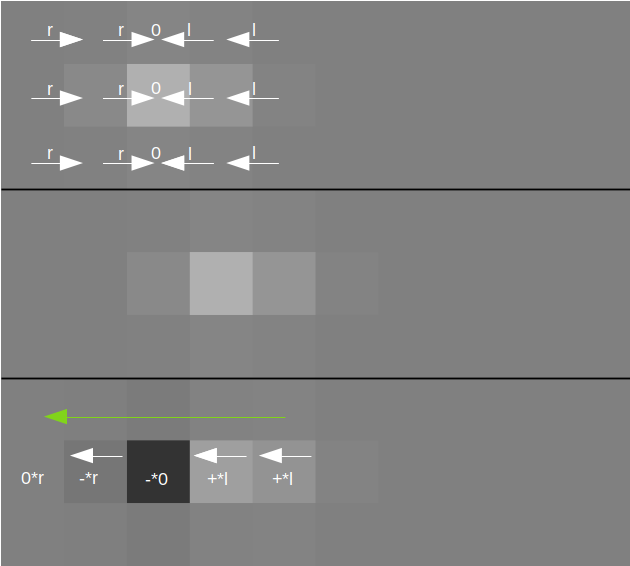
\includegraphics[height=0.2\textheight]{img/optical_flow_intuitive_1.png}}
  \quad
  \subfloat[]{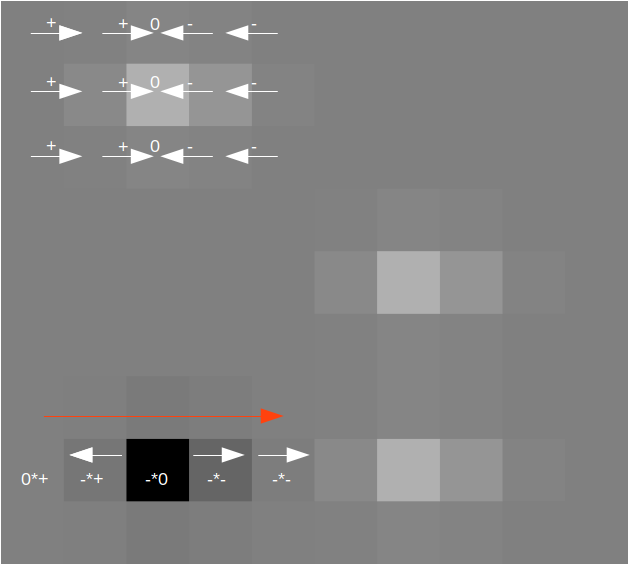
\includegraphics[height=0.2\textheight]{img/optical_flow_intuitive_2.png}}
  \quad
  \subfloat[]{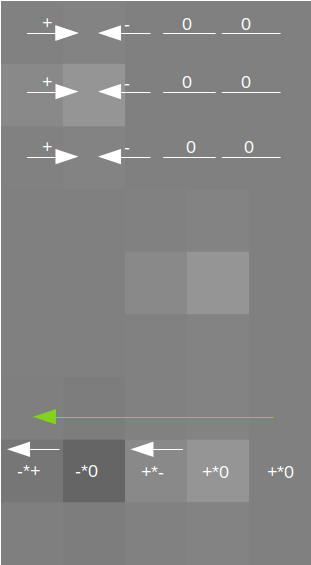
\includegraphics[height=0.2\textheight]{img/optical_flow_intuitive_3.png}}
  \caption{Optical Flow Intuitive see table \ref{tab:optical_flow_intuitive} for description}
  \label{fig:optical_flow_intuitive}
\end{figure}

\begin{table}[H]
   \centering
   \begin{tabular}{l l}
      Image a & Small move where we find the correct gradient green\\
      Image b & Bigger move where we find an invalid gradient red\\
      Image c & Bigger move as in b down-sampled in horizontal direction\\
      First row & Reference image with gradients\\
      Second row & Current image\\
      Last row & Diff image (current-reference)\\
      Color & Black -128, White +128\\
      l & Gradient points left\\
      r & Gradient points right\\
      + & Current pixel - reference pixel > 0\\
      - & Current pixel - reference pixel < 0\\
      Multiply & -*l=r,-*r=l\\
      Long arrow & Sum of gradients (e.g. l+l+l=l, r+r+l=r)
   \end{tabular}
   \caption{Optical Flow Intuitive Description}
   \label{tab:optical_flow_intuitive}
\end{table}


We extend the above scenario from a one-dimensional movement to a two-dimensional movement as shown in figure \ref{fig:optical_flow_2d}. This time we also calculate the gradient in the vertical direction. By doing so, we can track movements in x and y direction.

\begin{figure}[H]
  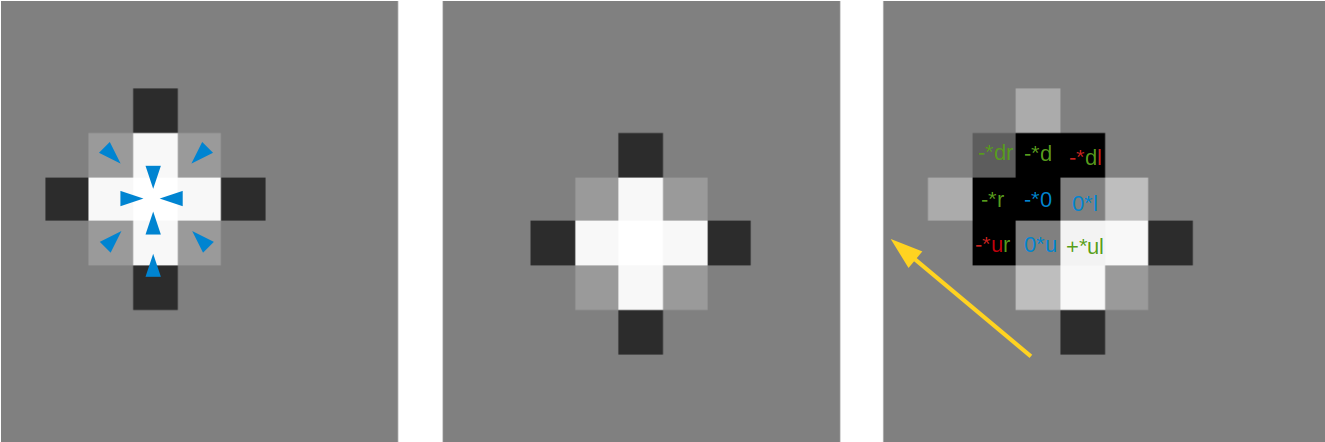
\includegraphics[width=1.0\textwidth]{img/optical_flow_2d.png}
  \caption{Optical Flow Intuitive 2D see table \ref{tab:optical_flow_2d} for description}
  \label{fig:optical_flow_2d}
\end{figure}

\begin{table}[H]
   \centering
   \begin{tabular}{l l}
       First column & Reference image with gradients\\
       Second column & Current image\\
       Third column & Diff image (current-reference)\\
       Color & Black -128, White +128\\
       + & Current-previous intensity > 0\\
       - & Current-previous intensity < 0\\
       u & Gradient points up\\
       d & Gradient points down\\
       l & Gradient points left\\
       r & Gradient points right\\
       Yellow arrow & Final gradient
  \end{tabular}
   \caption{Optical Flow Intuitive 2D Description}
  \label{tab:optical_flow_2d}
\end{table}

We showed that optical flow can track two dimensional movements. However, it doesn't track rotations and shearing effects. This will introduce dependencies between x and y movements which become non-linear. In the next section we extend the intuitive approach so that we can solve non-linear problems. Because these non-linearities are hard to show, we describe it mathematically.

\section{Lucas Kanade Mathematical}

In the previous section we showed the basic idea of optical flow. It is oversimplified and can only track movements in x and y direction. In this section we extend the idea to more complicated movements. Instead of linear movements in x and y direction we want to find a warp matrix which describes an affine transformation of a patch from one image to another (equation \ref{eq:lk_warp}).

\begin{equation}\label{eq:lk_warp}
  P=\begin{pmatrix}
    p_{11} & p_{12} & p_{13} \\
    p_{21} & p_{22} & p_{23}
  \end{pmatrix}
\end{equation}
\begin{align*}
  P       &:  \text{Warp matrix}\\
  p_{ij}  &:  \text{parameter of warp matrix}
\end{align*}
This warp matrix describes movements along the x and y axis($p_{11},p_{22}$), a rotation ($p_{13},p_{21}$) and shearing ($p_{13},p_{23}$). The goal of Lucas Kanade is to find this warp matrix. It does that by minimizing the intensity difference between a patch of pixels in the template (reference image) and a patch of pixels with the same size in the current image as shown in equation \ref{eq:lk_problem}. 

\begin{equation}\label{eq:lk_problem}
  \min_P(\sum_x^m\sum_y^n(I_{k}(x',y')-I_{k-1}(x(P),y(P)))^2)
\end{equation}
\begin{align*}
  m,n       &: \text{Patch size}\\
  x,y       &: \text{Pixel position in template}\\
  x',y'     &: \text{Pixel position in current image}\\
  I_{k-1}   &: \text{Template image}\\
  I_{k}     &: \text{Current image}\\
\end{align*}

We describe the transformation of a pixel from the reference image to the current image as a matrix multiplication as shown in equation \ref{eq:lk_warped}. Because \ref{eq:lk_problem} is a non-linear problem, we have to solve it with a non-linear solver (Gradient Descent). The problem is solved by iteratively changing the warp matrix in direction of the gradient until the difference of the intensities are minimal:
\begin{equation}\label{eq:lk_warped}
  \begin{gathered}
    \begin{pmatrix}
      x' \\
      y'
    \end{pmatrix}=
    W(x;P+\Delta P)\\
    =>
    \begin{pmatrix}
      p_{11}+\Delta p_{11} & p_{12}+\Delta p_{12} & p_{13}+\Delta p_{13} \\
      p_{21}+\Delta p_{21} & p_{22}+\Delta p_{22} & p_{23}+\Delta p_{23}
    \end{pmatrix}
    \begin{pmatrix}
      x\\
      y\\
      1
    \end{pmatrix}\\
    =>
    \begin{pmatrix}
      x(p_{11}+\Delta p_{11}) + y(p_{12}+\Delta p_{12}) + p_{13}+\Delta p_{13} \\
      x(p_{21}+\Delta p_{21}) + y(p_{22}+\Delta p_{22}) + p_{23}+\Delta p_{23}
    \end{pmatrix}
  \end{gathered}
\end{equation}
\begin{align*}
  W               &: \text{Warp function}\\
  \Delta p_{ij}   &: \text{change of $p_{ij}$ per iteration}
\end{align*}

After each iteration we set $P=P_{n-1}+\Delta P$ where P stands for all $p_{ij}$. We can solve this problem by approximating the gradient heuristically. However, this is slow. Therefore, we need a direct computational approach to find the gradient. This is what Lucas Kanade describes.\\
Equation \ref{eq:lk_problem} describes the Lucas Kanade problem which is non-linear. It is not possible to find $\Delta P$ algebraically which would be our gradient. Therefore, we need to linearise the problem by doing a first order Taylor approximation as shown in equation \ref{eq:lk_taylor} \cite{taylor_series}. $\nabla I$ is the exterior derivative when using the chain rule while $\frac{\sigma W}{\sigma P}$ is the inner derivative. 

\begin{equation}\label{eq:lk_taylor}
  \sum_x^m\sum_y^n(I_{k}(x_{i-1}',y_{i-1}')+\nabla I_{k}*\frac{\sigma W}{\sigma P}*\Delta P-I_{k-1}(x,y))^2
\end{equation}
\begin{align*}
  \nabla I_k  &:  \text{Intensity gradient in current image at position x',y'}
\end{align*}
We want to find $\Delta P$ which is our gradient. We derive equation \ref{eq:lk_taylor}. This gives us:
\begin{equation}
  2*\sum_x^m\sum_y^n\begin{bmatrix}\nabla I_{k}*\frac{\sigma W}{\sigma P}\end{bmatrix}^T*\begin{bmatrix}I_{k}(x_{i-1}',y_{i-1}')+\nabla I_{k}*\frac{\sigma W}{\sigma P}*\Delta P-I_{k-1}(x,y)\end{bmatrix}
\end{equation}
We now find $\Delta P$ by moving it to the left:
\tiny
\begin{equation}\label{eq:lk_dp}
  \Delta P=(\sum_x^m\sum_y^n\begin{bmatrix}\nabla I_{k}\frac{\sigma W}{\sigma P}\end{bmatrix}^T\begin{bmatrix}\nabla I_{k}\frac{\sigma W}{\sigma P}\end{bmatrix})^{-1}
  \sum_x^m\sum_y^n\begin{bmatrix}\nabla I_{k}\frac{\sigma W}{\sigma P}\end{bmatrix}^T\begin{bmatrix}I_{k-1}(x,y) - I_{k}(x_{i-1}',y_{i-1}'\end{bmatrix}
\end{equation}
\normalsize

We get $\frac{\sigma W}{\sigma P}$ by using equation \ref{eq:lk_warped} and do a partial derivation for each p. This gives us the Jacobian matrix shown in equation \ref{eq:lk_warped_derivative}.
\begin{equation}\label{eq:lk_warped_derivative}
  \frac{\sigma W}{\sigma P}=
  \begin{pmatrix}
    x & y & 1 & 0 & 0 & 0 \\
    0 & 0 & 0 & x & y & 1
  \end{pmatrix}
\end{equation}

We know all parameters in equation \ref{eq:lk_dp} and can calculate $\Delta P$. However, the following part of equation \ref{eq:lk_dp} is time consuming to calculate:
\begin{equation}
  H^{-1}=(\sum_x^m\sum_y^n\begin{bmatrix}\nabla I_{k}*\frac{\sigma W}{\sigma P}\end{bmatrix}^T*\begin{bmatrix}\nabla I_{k}*\frac{\sigma W}{\sigma P}\end{bmatrix})^{-1}
\end{equation}
We call $H$ the Hessian matrix. It is the same formulation used by Gauss-Newton optimization. Therefore, this is the optimization method of choice for finding the minima. We need to calculate the Hessian matrix for each iteration. Because this is time consuming, we normally use the Inverse Compositional Lucas Kanade algorithm. It tries to solve the problem by warping the template to the current image instead of the current image to the template. We see that in the next section.

\section{Inverse Compositional Lucas Kanade}\label{sec:inv_comp_lk}
The problem the Inverse Compositional Lucas Kanade algorithm solves stays the same as before. However, we switch the role of the template and the image as shown in equation \ref{eq:iclk_problem}.
\begin{equation}\label{eq:iclk_problem}
  \min_P(\sum_x^m\sum_y^n(I_{k-1}(x''(P),y''(P))-I_{k}(x',y'))^2)
\end{equation}
\begin{align*}
  m,n        &: \text{Patch size}\\
  x'',y''    &: \text{Warped pixel position in the template}\\
  x',y'      &: \text{Pixel position in the current image}\\
  I_{k-1}    &: \text{Template image}\\
  I_{k}      &: \text{Current image}\\
  P          &: \text{Warp matrix see \ref{eq:lk_warp}}
\end{align*}

This time we warp the template with $\Delta P$ as shown in equation \ref{eq:inv_lk_warp}. 
\begin{equation}\label{eq:inv_lk_warp}
  \begin{gathered}
    \begin{pmatrix}
      x'' \\
      y''
    \end{pmatrix}=
    W(x;\Delta P)\\
    =>\begin{pmatrix}
      1 + \Delta p_{11} & 0 + \Delta p_{12} & 0 + \Delta p_{13} \\
      0 + \Delta p_{21} & 1 + \Delta p_{22} & 0 + \Delta p_{23}
    \end{pmatrix}
    \begin{pmatrix}
      x\\
      y\\
      1
    \end{pmatrix}\\
    \begin{pmatrix}
      x' \\
      y'
    \end{pmatrix}=
    \begin{pmatrix}
      p_{11} & p_{12} & p_{13} \\
      p_{21} & p_{22} & p_{23}
    \end{pmatrix}*
    \begin{pmatrix}
      x\\
      y\\
      1
    \end{pmatrix}
  \end{gathered}
\end{equation}
\begin{align*}
  x,y            &: \text{Original pixel position in the template}\\
  x'',y''        &: \text{Warped pixel position in the template}\\
  p_{ij}         &: \text{parameter of warp matrix}\\
  \Delta p_{ij}  &: \text{change of $p_{ij}$ per iteration}
\end{align*}


We separate the update step from the warping of the image. We now show the update step in equation \ref{eq:iclk_update}. Note that the update step is not additive as for Lucas Kanade. We can argue this is because the new warp depends on the old warps rotation. We can express this with the matrix multiplication shown in equation \ref{eq:iclk_update}.
\begin{equation}\label{eq:iclk_update}
  \begin{gathered}
    W(x;p)=W(W(x;\Delta P)^{-1}; p)\\
    =>
    \begin{pmatrix}
    p_{11} & p_{12} & p_{13} \\
    p_{21} & p_{22} & p_{23}
    \end{pmatrix}
    \begin{pmatrix}
      \Delta p_{11} & \Delta p_{12} & \Delta p_{13} \\
      \Delta p_{21} & \Delta p_{22} & \Delta p_{23}
    \end{pmatrix}
    \begin{pmatrix}
      x\\
      y\\
      1
    \end{pmatrix}
  \end{gathered}
\end{equation}
\begin{align*}
  W               &: \text{Warp function}\\
  \Delta P        &: \text{Update of warp matrix}
\end{align*}

From equation \ref{eq:iclk_problem} we need to do the first order Taylor approximation as we did for the normal Lucas Kanade algorithm (equation \ref{eq:iclk_taylor}).
\begin{equation}\label{eq:iclk_taylor}
  \sum_x^m\sum_y^m(I_{k-1}(x,y)+\nabla I_{k-1}*\frac{\sigma W}{\sigma P}*\Delta P-I_{k}(x',y'))^2
\end{equation}
\begin{align*}
  \nabla I_{k-1}  &:  \text{Intensity gradient in template at position x,y}
\end{align*}

We derive equation \ref{eq:iclk_taylor} and set it to zero to minimize the problem (equation \ref{eq:iclk_derivative}).
\begin{equation}\label{eq:iclk_derivative}
  2\sum_x^m\sum_y^n\begin{bmatrix}\nabla I_{k-1}\frac{\sigma W}{\sigma P}\end{bmatrix}^T\begin{bmatrix}I_{k}(x_{i-1}',y_{i-1}')+\nabla I_{k-1}\frac{\sigma W}{\sigma P}\Delta P-I_{k-1}(x,y)\end{bmatrix}
\end{equation}

This allows us to find the gradient $\Delta P$ (equation \ref{eq:iclk_dp}) for the non-linear optimization.
\tiny
\begin{equation}\label{eq:iclk_dp}
  \Delta P=(\sum_x\sum_y\begin{bmatrix}\nabla I_{k-1}\frac{\sigma W}{\sigma P}\end{bmatrix}^T\begin{bmatrix}\nabla I_{k-1}\frac{\sigma W}{\sigma P}\end{bmatrix})^{-1}
  \sum_x^m\sum_y^n\begin{bmatrix}\nabla I_{k-1}\frac{\sigma W}{\sigma P}\end{bmatrix}^T\begin{bmatrix}I_{k}(x_{i-1}',y_{i-1}') - I_{k-1}(x,y)\end{bmatrix}
\end{equation}
\normalsize

Compared to the normal Lucas-Kanade algorithm, the Hessian Matrix H is now constant for all iterations.
\begin{equation}
  \Delta H=\sum_x^m\sum_y^n\begin{bmatrix}\nabla I_{k-1}*\frac{\sigma W}{\sigma P}\end{bmatrix}^T*\begin{bmatrix}\nabla I_{k-1}*\frac{\sigma W}{\sigma P}\end{bmatrix}
\end{equation}

Because we only have to calculate the Hessian matrix once, the Inverse Compositional Lucas Kanade is more efficient than the Lucas Kanade algorithm.\\
We use Inverse Compositional Lukas Kanade in SVO to calculate the optical flow for pose refinement. In the next section we describe how we can use optical flow to find a 3D pose instead of a warp matrix. This is what we need for sparse image alignment in SVO.

\section{Sparse Image Alignment}\label{sec:pose_estimation}
We use a slightly different optical flow method to get a first estimate of the pose in SVO. Instead of searching a warp matrix we directly optimize a 3D pose. We start again with the idea of minimizing the intensity differences over a patch of pixels shown in equation \ref{eq:pe_problem}.
\begin{equation}\label{eq:pe_problem}
  \min_P(\sum_{a \in A}\sum_{x=a_x-\frac{m}{2}}^m\sum_{y=a_y-\frac{n}{2}}^n(I_{k-1}(x''(P),y''(P))-I_{k}(x',y'))^2)
\end{equation}
\begin{align*}
  m,n       &: \text{Patch size}\\
  x'',y''   &: \text{Warped pixel position in the template}\\
  x',y'     &: \text{Pixel position in the current image}\\
  I_{k-1}   &: \text{Template image}\\
  I_{k}     &: \text{Current image}\\
  A         &: \text{For all keypoints a}\\
  P         &: \text{Projection matrix \ref{eq:pe_warped}}
\end{align*}

This time we use 3D points instead of pixel positions. Therefore, we use a projection matrix instead of a warp matrix. The projection matrix $P$ is shown in equation \ref{eq:pe_warped}. 

\begin{equation}\label{eq:pe_warped}
  \begin{split}
  \begin{pmatrix}
    u \\
    v \\
    s
  \end{pmatrix}=
  \begin{pmatrix}
    f_x & 0 & c_x \\
    0 & f_y & c_y \\
    0 & 0 & 1
  \end{pmatrix}*
  \begin{pmatrix}
    r_{11} & r_{12} & r_{13} & t_x \\
    r_{21} & r_{22} & r_{23} & t_y \\
    r_{31} & r_{32} & r_{33} & t_z
  \end{pmatrix}*
  \begin{pmatrix}
    X\\
    Y\\
    Z\\
    1
  \end{pmatrix}\\
  =>\begin{pmatrix}
    p_{11} & p_{12} & p_{13} & p_{14} \\
    p_{21} & p_{22} & p_{23} & p_{24} \\
    p_{31} & p_{32} & p_{33} & p_{34}
  \end{pmatrix}*
  \begin{pmatrix}
    X\\
    Y\\
    Z\\
    1
  \end{pmatrix}\\
  =>P*G
\end{split}
\end{equation}
\begin{align*}
  u,v,s     &: \text{Scaled pixel position}\\
  X,Y,Z     &: \text{3D Point position}\\
  x,y       &: \text{2D Point position in image}\\
  p_{ij}    &: \text{Parameters of projection matrix P}\\
  r_{ij}    &: \text{Rotation matrix}\\
  t_{x,y,z} &: \text{Translation}\\
  f_x,f_y   &: \text{Focal length}\\
  c_x,c_y   &: \text{Principal point}\\
  P         &: \text{Projection matrix}\\
  G         &: \text{3D Point position (vector)}
\end{align*}

We need to find 12 gradients if we use the formulation in equation \ref{eq:pe_projection} for the inverse compositional Lucas Kanade. However, the rotational factors $r_{nm}$ in equation \ref{eq:pe_warped} depend on each other. We could express the whole matrix based on 6 unknowns which are 3 times rotation and 3 times translation. It is easy to see that this formulation gets rather complex and it is untraceable to find a Jacobian for such a matrix.\\
\begin{equation}\label{eq:pe_projection}
  \begin{gathered}
    \begin{pmatrix}
      x' \\
      y' 
    \end{pmatrix}=
    \begin{pmatrix}
      \frac{u}{s} \\
      \frac{v}{s} 
    \end{pmatrix}=
    \begin{pmatrix}
      \frac{p_{11}*X + p_{12}*Y + p_{13}*Z + p_{14}}{p_{31}*X + p_{32}*Y + p_{33}*Z + p_{34}}  \\
      \frac{p_{21}*X + p_{22}*Y + p_{23}*Z + p_{24}}{p_{31}*X + p_{32}*Y + p_{33}*Z + p_{34}}
    \end{pmatrix}\\
    \begin{pmatrix}
      x'' \\
      y'' 
    \end{pmatrix}=W(X,Y,Z;\Delta P)\\
    =>\begin{pmatrix}
      \frac{u''}{s''} \\
      \frac{v''}{s''} 
    \end{pmatrix}=
    \begin{pmatrix}
      \frac{\Delta p_{11}*X + \Delta p_{12}*Y + \Delta p_{13}*Z + \Delta p_{14}}{\Delta p_{31}*X + \Delta p_{32}*Y + \Delta p_{33}*Z + \Delta p_{34}}  \\
      \frac{\Delta p_{21}*X + \Delta p_{22}*Y + \Delta p_{23}*Z + \Delta p_{24}}{\Delta p_{31}*X + \Delta p_{32}*Y + \Delta p_{33}*Z + \Delta p_{34}}
    \end{pmatrix}\\
  \end{gathered}
\end{equation}
\begin{align*}
  \Delta p_{ij}   &: \text{Update of projection parameters}\\
  \Delta P        &: \text{Update of projection matrix}
\end{align*}

We reformulate the problem by using Lie algebra \cite{se3_explain}. We use two terms SE(3) and se(3). SE(3) describes our ``normal'' projection matrices with a rotational and transitional part as shown in equation \ref{eq:pe_warped}. If we use Lie algebra, we write se(3) instead of SE(3). We move from se(3) to SE(3) by using the exponential map and from SE(3) to se(3) by using the logarithm map. The problem we need to solve stays the same as in equation \ref{eq:pe_problem}. However, we need to find $x''$ and $y''$ differently. We use the following formulation:
\begin{equation}\label{eq:pe_lie}
  \begin{gathered}
    \begin{pmatrix}
      x''\\
      y''
    \end{pmatrix}
    =h(e^{\xi}*G)\\
    \xi=\begin{pmatrix}
      v_x\\
      v_y\\
      v_z\\
      \omega_x\\
      \omega_y\\
      \omega_z
    \end{pmatrix}
  \end{gathered}
\end{equation}
\begin{align*}
  h                            &: \text{Mapping function from u,v,s to x,y}\\
  e                            &: \text{Exponential map}\\
  \xi                          &: \text{Pose gradient as vector in se(3)}\\
  v_x,v_y,v_z                  &: \text{Position change in se3}\\
  \omega_x,\omega_y,\omega_z   &: \text{Angle change in se3}
\end{align*}

$\xi$ in \ref{eq:pe_lie} is the change in angle and position in se(3). We can transfer from se(3) back to SE(3) by using the exponential map $e$. The exponential map is the pendant to the Euler function for matrices. In our case it has the closed form solution shown in \ref{eq:pe_closed_form} \cite{rvc}.

\begin{equation}\label{eq:pe_closed_form}
  \begin{gathered}
    \omega_{skew}=\begin{pmatrix}
      0 && -\omega_z && \omega_y \\
      \omega_z && 0 && -\omega_x \\
      -\omega_y && \omega_x && 0
    \end{pmatrix}\\
    \begin{pmatrix}
      \Delta t_x\\
      \Delta t_y\\
      \Delta t_z
    \end{pmatrix}=
    I+(1-cos(1))w_{skew}+(1-sin(1))*w_{skew}^2*\begin{pmatrix}
      v_x\\
      v_y\\
      v_z
    \end{pmatrix}\\
    \begin{pmatrix}
      \Delta r_x\\
      \Delta r_y\\
      \Delta r_z
    \end{pmatrix}=
    \begin{pmatrix}
      \omega_x\\
      \omega_y\\
      \omega_z
    \end{pmatrix}
  \end{gathered}
\end{equation}
\begin{align*}
  \Delta t_{x,y,z}    &: \text{Translational update step}\\
  \Delta r_{x,y,z}    &: \text{Rotational update step}
\end{align*}

We use $\Delta t_x,\Delta t_y,\Delta t_z,\Delta r_x,\Delta r_y,\Delta r_z$ as our gradient to update the pose. We need to rotate the gradient by the current pose because we use the Inverse Compositional Lucas Kanade algorithm (see \ref{sec:inv_comp_lk}). We show the update step in equation \ref{eq:pe_update}.
\begin{equation}\label{eq:pe_update}
  \begin{gathered}
    \begin{pmatrix}
      t_x\\
      t_y\\
      t_z
    \end{pmatrix}=
    \begin{pmatrix}
      t_x\\
      t_y\\
      t_z
    \end{pmatrix}+
    \begin{pmatrix}
      r_{11} & r_{12} & r_{13}\\
      r_{21} & r_{22} & r_{23}\\
      r_{31} & r_{32} & r_{33}
    \end{pmatrix}*
    \begin{pmatrix}
      \Delta t_x\\
      \Delta t_y\\
      \Delta t_z
    \end{pmatrix}\\
    \begin{pmatrix}
      r_x\\
      r_y\\
      r_z
    \end{pmatrix}=
    \begin{pmatrix}
      r_x\\
      r_y\\
      r_z
    \end{pmatrix}+
    \begin{pmatrix}
      r_{11} & r_{12} & r_{13}\\
      r_{21} & r_{22} & r_{23}\\
      r_{31} & r_{32} & r_{33}
    \end{pmatrix}*
    \begin{pmatrix}
      \Delta r_x\\
      \Delta r_y\\
      \Delta r_z
    \end{pmatrix}
  \end{gathered}
\end{equation}

To get $\xi$ we again do the first order Taylor approximation as shown in equation \ref{eq:pe_taylor}.
\begin{equation}\label{eq:pe_taylor}
  \sum_x^m\sum_y^n(I_{k-1}(x,y)+\nabla I_{k-1}*\frac{\sigma h(e^{\xi}*G)}{\sigma \xi}*\xi-I_{k}(x',y'))^2
\end{equation}
\begin{align*}
  x,y          &: \text{Original pixel position in template}\\
  \nabla I     &: \text{Gradient in image I at position x',y'}\\
\end{align*}

We again derive equation \ref{eq:pe_taylor} from $\xi$ and set it to zero as shown in equation \ref{eq:pe_derivative}. This finally allows us to find $\xi$.

\begin{equation}\label{eq:pe_derivative}
  2\sum_x^m\sum_y^n\begin{bmatrix}\nabla I_{k-1}\frac{\sigma h(e^{\xi}G)}{\sigma \xi}\end{bmatrix}^T\begin{bmatrix}I_{k}(x_{i-1}',y_{i-1}')+\nabla I_{k-1}\frac{\sigma h(e^{\xi} G)}{\sigma \xi}\xi-I_{k-1}(x,y)\end{bmatrix}
\end{equation}

We want to find $\xi$ which leads us to equation \ref{eq:pe_xi}.

\tiny
\begin{equation}\label{eq:pe_xi}
  \xi=(\sum_x^m\sum_y^n\begin{bmatrix}\nabla I_{k-1}\frac{\sigma h(e^{\xi}G)}{\sigma \xi}\end{bmatrix}^T\begin{bmatrix}\nabla I_{k-1}\frac{\sigma h(e^{\xi}G)}{\sigma \xi}\end{bmatrix})^{-1}
  \sum_x^m\sum_y^n\begin{bmatrix}\nabla I_{k-1}\frac{\sigma h(e^{\xi}G)}{\sigma \xi}\end{bmatrix}^T\begin{bmatrix}I_{k}(x_{i-1}',y_{i-1}') - I_{k-1}(x,y)\end{bmatrix}
\end{equation}
\normalsize

We have to find a solution for $\frac{\sigma h(e^{\xi}G)}{\sigma \xi}$ to calculate $\xi$. This Jacobian matrix is shown in equation \ref{eq:se3_jacobian} (see \cite{se3_explain} for derivation).
\begin{equation}\label{eq:se3_jacobian}
  \frac{h(e^{\xi}G)}{\delta \xi}=
  \begin{pmatrix}
    f_x & f_y
  \end{pmatrix}
  \begin{pmatrix}
    \frac{1}{Z} & 0 & -\frac{X}{z^2} & -\frac{X*Y}{Z^2} & 1 + \frac{X^2}{Z^2} & -\frac{Y}{Z} \\
    0 & \frac{1}{Z}  & -\frac{Y}{z^2} & -1 - \frac{Y^2}{Z^2} & \frac{X*Y}{Z^2} &  \frac{X}{Z}
  \end{pmatrix}
\end{equation}

Given the Jacobian and all 3D points, we can calculate the gradient for a given pose. We then iteratively optimize the pose based on the gradient as we did for the Inverse Compositional Lucas Kanade algorithm. We can use image pyramids to track bigger movements. Instead of one optimization we do an optimization round for each pyramid level.

\chapter{Pose Refinement}\label{ch:pose_refinement}

We use pose refinement in SVO to decrease the drift over time and to increase the accuracy of the sparse image alignment. In a first step we use Inverse Compositional Lucas Kanade to locate keypoints in the current image. Then we try to minimize the re-projection error shown in equation \ref{eq:refinement_reprojection}.
\begin{equation}\label{eq:refinement_reprojection}
  \begin{gathered}
    \min_P(\sum_{a \in A|x'=a_x,y'=a_y}((x'-x(P))^2+(y'-y(P))^2))\\
    =>\min_P(\sum_{a \in A|g=a}((g'-g(P))^T(g'-g(P)))
  \end{gathered}
\end{equation}
\begin{align*}
  x',y'   &: \text{2D Point position found by optical flow}\\
  x,y     &: \text{2D Point projected from 3D (see \ref{eq:camera_model})}\\
  g,g'    &: \text{x,y and x',y' as vector}\\
  P       &: \text{Projection matrix}\\
  A       &: \text{For all keypoints}\\
\end{align*}

We can achieve that with heuristic gradient descent but it's not efficient. Therefore, we use a similar approach as we use for optical flow. We try to find the gradient mathematically. Based on the camera model we use the formulation shown in equation \ref{eq:refinement_projection} for optimization. As we saw for pose estimation, we can not use this formulation directly because we can not find a Jacobian.

\begin{equation}\label{eq:refinement_projection}
  \begin{gathered}
    \begin{pmatrix}
      x \\
      y 
    \end{pmatrix}=
    \begin{pmatrix}
      \frac{u}{s} \\
      \frac{v}{s} 
    \end{pmatrix}=
    \begin{pmatrix}
      \frac{(p_{11} + \Delta p_{11})*X + (p_{12} + \Delta p_{12})*Y + (p_{13} + \Delta p_{13})*Z + (p_{14} + \Delta p_{14})}{(p_{31}+\Delta p_{31})*X + (p_{32} + \Delta p_{32})*Y + (p_{33} + \Delta p_{33})*Z + (p_{34} + \Delta p_{34})}  \\
      \frac{(p_{21} + \Delta p_{21})*X + (p_{22} + \Delta p_{22})*Y + (p_{23} + \Delta p_{23})*Z + (p_{24} + \Delta p_{24})}{(p_{31}+\Delta p_{31})*X + (p_{32} + \Delta p_{32})*Y + (p_{33} + \Delta p_{33})*Z + (p_{34} + \Delta p_{34})}
    \end{pmatrix}
  \end{gathered}
\end{equation}
\begin{align*}
  u,v,s           &:  \text{Pixel position scaled with s}\\
  X,Y,Z           &:  \text{3D Pixel position}\\
  p_{ij}          &:  \text{Projection parameters}\\
  \Delta p_{ij}   &:  \text{Projection parameter change per iteration}\\
\end{align*}

We formulate the problem with the help of Lie algebra as shown in equation \ref{eq:refinement_lie}.
\begin{equation}\label{eq:refinement_lie}
  \begin{gathered}
    \begin{pmatrix}
      x\\
      y
    \end{pmatrix}
    =h(e^{\xi}*G)\\
    \xi=\begin{pmatrix}
      v_x\\
      v_y\\
      v_z\\
      \omega_x\\
      \omega_y\\
      \omega_z
    \end{pmatrix}
  \end{gathered}
\end{equation}
\begin{align*}
  P     &: \text{Current projection matrix}\\
  e     &: \text{Exponential map}\\
  \xi   &: \text{Pose gradient as vector in se(3)}\\
  G     &: \text{3D point}\\
  h     &: \text{Mapping function from u,v,s to x,y}
\end{align*}

If we formulate the problem of equation \ref{eq:refinement_reprojection} with the knowledge of equation \ref{eq:refinement_lie}, we end in equation \ref{eq:refinement_solve}.

\begin{equation}\label{eq:refinement_solve}
  \begin{gathered}
    \sum_n ((g'-g)^T(g'-g))\\
    =>\sum_n (g'-h(e^{\xi}*G))^2
  \end{gathered}
\end{equation}

We do a Taylor approximation of the inner part as shown in equation \ref{eq:refinement_taylor}.
\begin{equation}\label{eq:refinement_taylor}
  (g'-h(e^{\xi}*G)+\frac{h(e^{\xi}*G)}{\xi}(\xi))^2
\end{equation}

Now we derive the Taylor approximation, which is shown in equation \ref{eq:refinement_derived}.
\begin{equation}\label{eq:refinement_derived}
  \begin{gathered}
    (\frac{h(e^{\xi}*G)}{\xi})^T2*(g'-h(e^{\xi}*G)+\frac{h(e^{\xi}*G)}{\xi}(\xi))=0\\
    (\frac{h(e^{\xi}*G)}{\xi})^T(g'-h(e^{\xi}*G))+\frac{h(e^{\xi}*G)}{\xi}\frac{h(e^{\xi}*G)}{\xi}\xi=0\\
    ((\frac{h(e^{\xi}*G)}{\xi})^T(\frac{h(e^{\xi}*G)}{\xi}))^{-1}(\frac{h(e^{\xi}*G)}{\xi})^T(h(e^{\xi}*G)-g')=\xi
  \end{gathered}
\end{equation}

We use the same definition for the Jacobian as we did for Sparse Image Alignment in equation \ref{eq:se3_jacobian}. To get the gradient in SE(3) we use equation \ref{eq:pe_closed_form}. However, the resulting $\Delta t_x,\Delta t_y,\Delta t_z,\Delta r_x,\Delta r_y,\Delta r_z$ are already our update steps. We don't have to multiply the gradient with the current rotation matrix as we did in section \ref{sec:pose_estimation}.

\chapter{Implementation}\label{ch:implementation}
In this chapter, we discuss how we implemented the algorithm during this thesis. It should give a rough overview of the code base. All the source code written during this thesis is available on Github under the following link:\\
\url{https://github.com/eichenberger/stereo-svo-slam}

We organized the repository as follows:
\begin{table}[H]
  \centering
  \begin{tabular}{|l|l|}
    Directory & Description\\
    \hline
    doc & Documentation (current document)\\
    src  & The source code\\
    src/app & The source code for the test application\\
    src/ar-app & The source code for the demo augmented reality app\\
    src/lib & The source code for the library\\
    src/python & The source code for the python wrapper and python demo\\
    src/qt-viewer & The source code for the Qt 3D Viewer\\
    test & Some test and helper scripts
  \end{tabular}
\caption{Repository organization}
\label{tab:organization}
\end{table}

The source code uses GNU Makefiles for compilation. Table \ref{tab:envvars} shows the environment variables used to control the make process.
\begin{table}[H]
  \centering
  \begin{tabular}{|l|l|}
    Variable & Description\\
    \hline
    OPENCV\_INC\_DIR & Include directory for OpenCV (opencv2/..)\\
    OPENCV\_LIB\_DIR & Where to find the opencv libraries if not in standard path\\
    QT\_INC\_DIR & Where to find the Qt include files if not in standard path\\
    QMAKE & Which qmake should be used\\
    CXX & Which compiler should be use\\
    CXXFLAGS & Additional compiler flags (e.g. -O0/-O3)\\
    LDFLAGS & Additional linker flags (e.g.  additional library paths)
  \end{tabular}
\caption{Environment variables for GNU Make}
\label{tab:envvars}
\end{table}

The following make commands are available under the src directory:
\begin{lstlisting}
# Compile library, app (test applicaiton) and ar-app (demo application)
make 
# Compile the python wrapper
make python 
# Compile the qt-viewer
make qt-viewer
\end{lstlisting}

All applications besides the qt-viewer accepts some command line arguments. It is possible to query the help text by calling the application with -h:\\
\begin{lstlisting}
./slam_app -h
Usage: ./slam_app [options] camera
SVO stereo SLAM application

Options:
  -h, --help                     Displays this help.
  -v, --video <video>            Path to camera or video (/dev/videoX,
                                 video.mov)
  -s, --settings <settings>      Path to the settings file (Econ.yaml)
  -r, --hidraw <hidraw>          econ: HID device to control the camera
                                 (/dev/hidrawX)
  -i, --hidrawimu <hidrawimu>    econ: HID device to control the imu
                                 (/dev/hidrawX)
  -e, --exposure <exposure>      econ: The exposure for the camera 1-30000
  -t, --trajectory <trajectory>  File to store trajectory
  -m, --move <move>              video: skip first n frames
  -d, --hdr                      econ: Use HDR video

Arguments:
  camera                         The camera type to use can be econ, video or
                                 euroc
\end{lstlisting}

Most applications require a camera settings file which describes the camera parameters and algorithm settings. We provide an example file for Blender including comments under src/app/Blender.yaml.

\section{Library}

We wrote the stereo SVO Library (libstereosvo) as a shared library. We can use it in other projects by dynamically linking against it.
\begin{figure}[H]
  \centering
  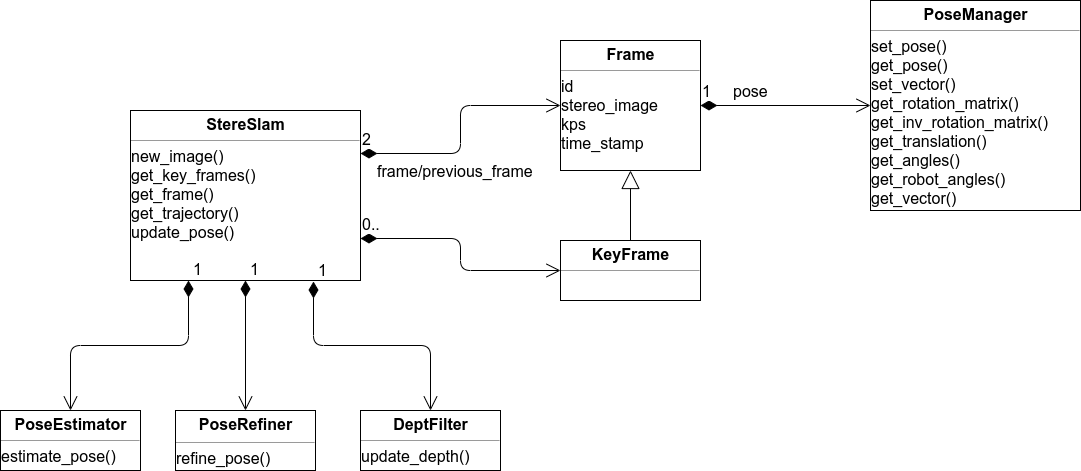
\includegraphics[width=1.0\textwidth]{img/class_diagram.png}
  \caption{Class diagram for the Stereo SVO Library}\label{fig:class_diagram}
\end{figure}

In figure \ref{fig:class_diagram} we show the most important classes of the library. To start the SLAM system we create an instance of StereoSlam. When we create the object we need to specify the camera parameters (see software documentation in appendix). After that we feed new images by calling the method new\_image. The getter functions are used to get the current frame (with pose information), all keyframes (including keypoints), the trajectory or to update the pose.

\subsection{Stereo SLAM}

The Stereo SLAM class implements the basic algorithm described in \ref{ch:svo} and shown in \ref{fig:svo_slam}. Figure \ref{fig:flow_stereo_slam} shows a slightly changed flow chart to align better with the naming in the implementation. It calls the depth calculator if new keyframes are needed, estimates the pose and updates the point cloud. However, it delegates the work to its sub objects. It also provides an interface to receive information about the current state (see figure \ref{fig:class_diagram}).

\begin{figure}[H]
  \centering
  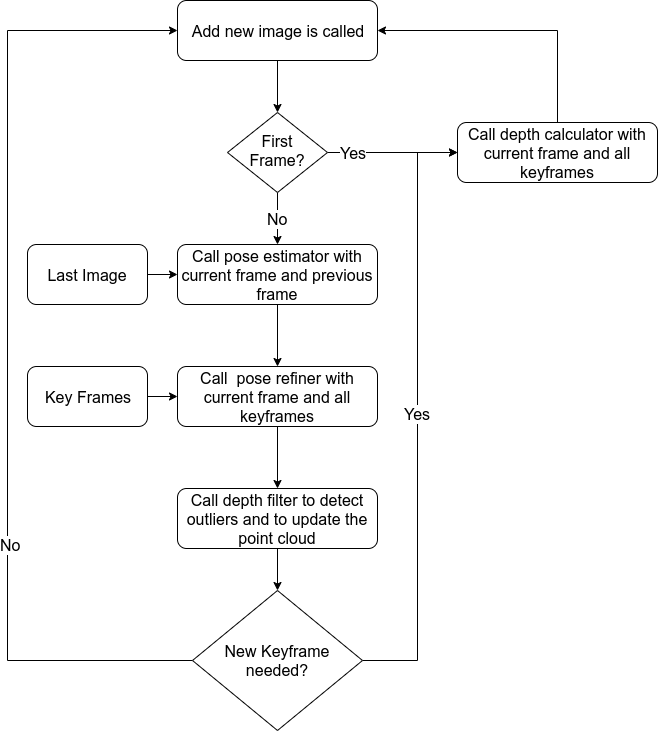
\includegraphics[scale=0.3]{img/flow_stereo_slam.png}
  \caption{Stereo SLAM Flow}\label{fig:flow_stereo_slam}
\end{figure}


\subsection{Depth Calculator}

The depth calculator divides the image into grids and searches for new keypoints, merges keypoints from previous keyframes and estimates the depth. It is only used when a new keyframe is required. Figure \ref{fig:flow_depth_calculator} shows the flow diagram of the depth calculation.

\begin{figure}[H]
  \centering
  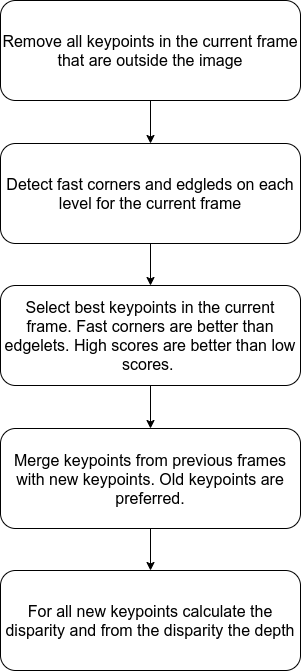
\includegraphics[scale=0.3]{img/flow_depth_calculator.png}
  \caption{Depth Calculator Flow}\label{fig:flow_depth_calculator}
\end{figure}

\subsection{Pose Estimator}

The pose estimator does a first estimate of the pose, based on the previous image. It does that by using sparse image alignment described in section \ref{sec:sia}. Figure \ref{fig:flow_pose_estimator} shows the flow diagram for the pose estimator.

\begin{figure}[H]
  \centering
  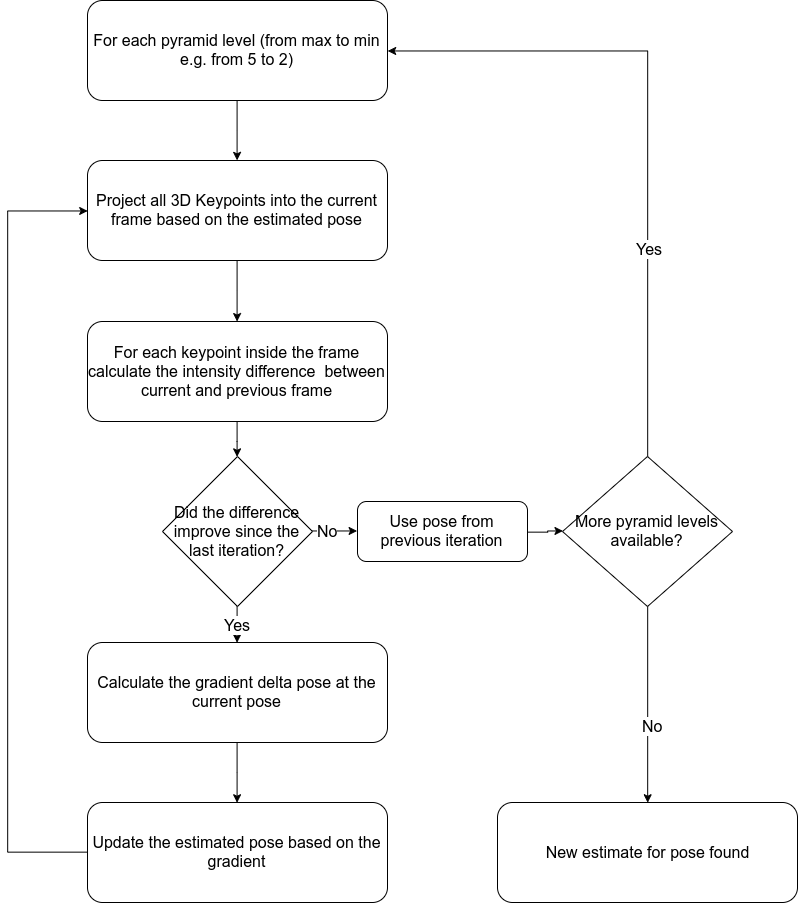
\includegraphics[scale=0.3]{img/flow_pose_estimator.png}
  \caption{Pose Estimator Flow}\label{fig:flow_pose_estimator}
\end{figure}

\subsection{Pose Refiner}

The pose refiner updates the pose by using the keyframes where a keypoint was first seen. This reduces the drift over time. It uses the algorithm described in chapter \ref{ch:pose_refinement}. Figure \ref{fig:flow_pose_refiner} shows the flow diagram of the pose refiner.

\begin{figure}[H]
  \centering
  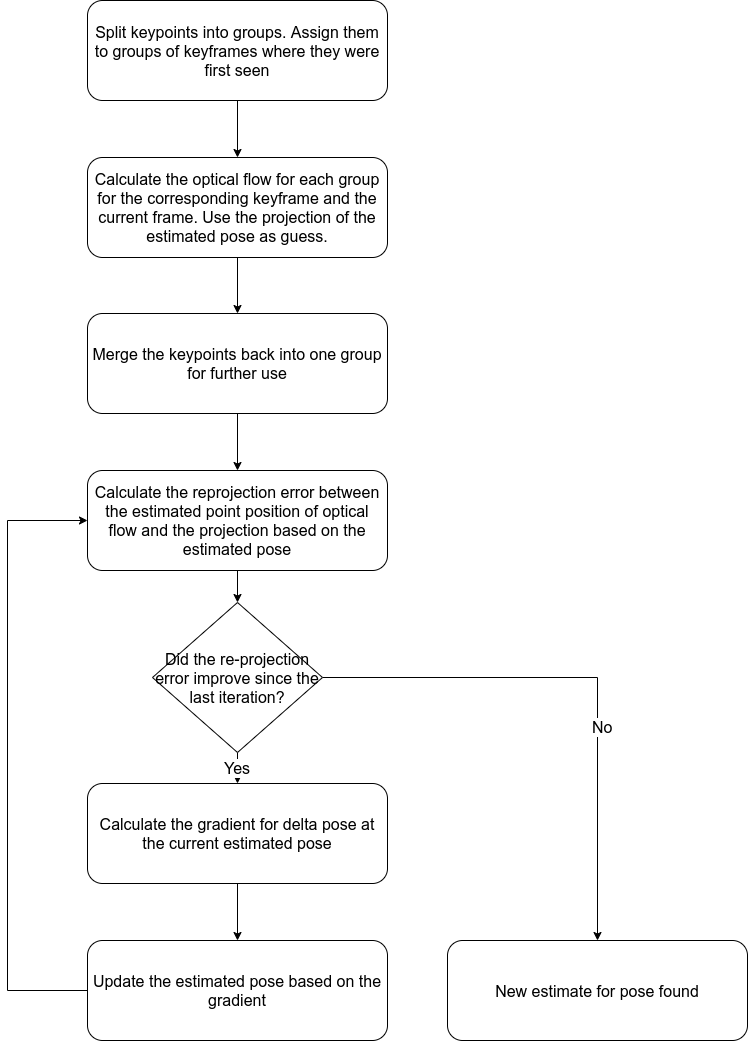
\includegraphics[scale=0.3]{img/flow_pose_refiner.png}
  \caption{Pose Refiner Flow}\label{fig:flow_pose_refiner}
\end{figure}

\subsection{Depth Filter}\label{sec:depth_filter}

The depth filter removes outlier and updates the 3D point position of keypoints as described in section \ref{sec:point_update}. Figure \ref{fig:flow_depth_filter} shows two flows. The first flow a describes the outlier detection while the second flow b describes the 3D point update.

\begin{figure}[H]
  \centering
  \subfloat[Outlier detecction]{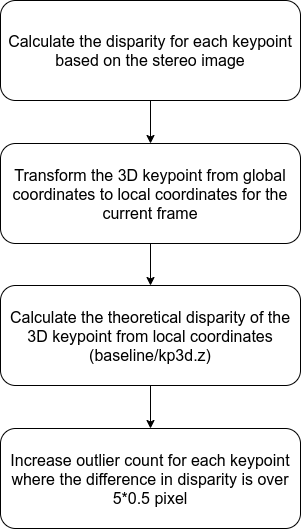
\includegraphics[scale=0.3]{img/flow_depth_filter_outlier.png}}
  \qquad
  \subfloat[3D Point Update]{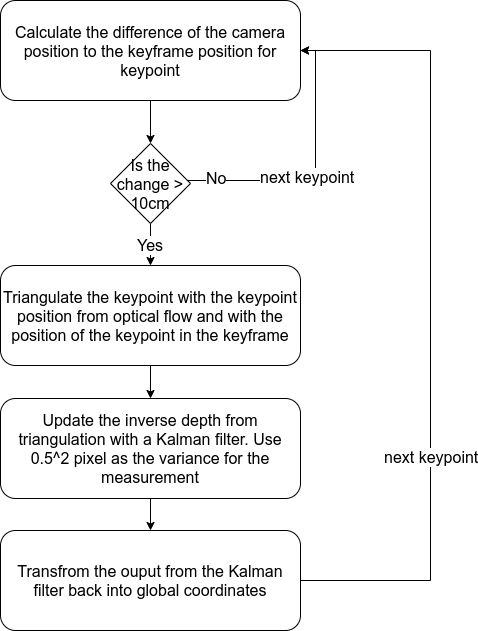
\includegraphics[scale=0.3]{img/flow_depth_filter_update.png}}
  \caption{Depth Filter Flow}\label{fig:flow_depth_filter}
\end{figure}

\section{Test Application}

\begin{figure}[H]
  \centering
  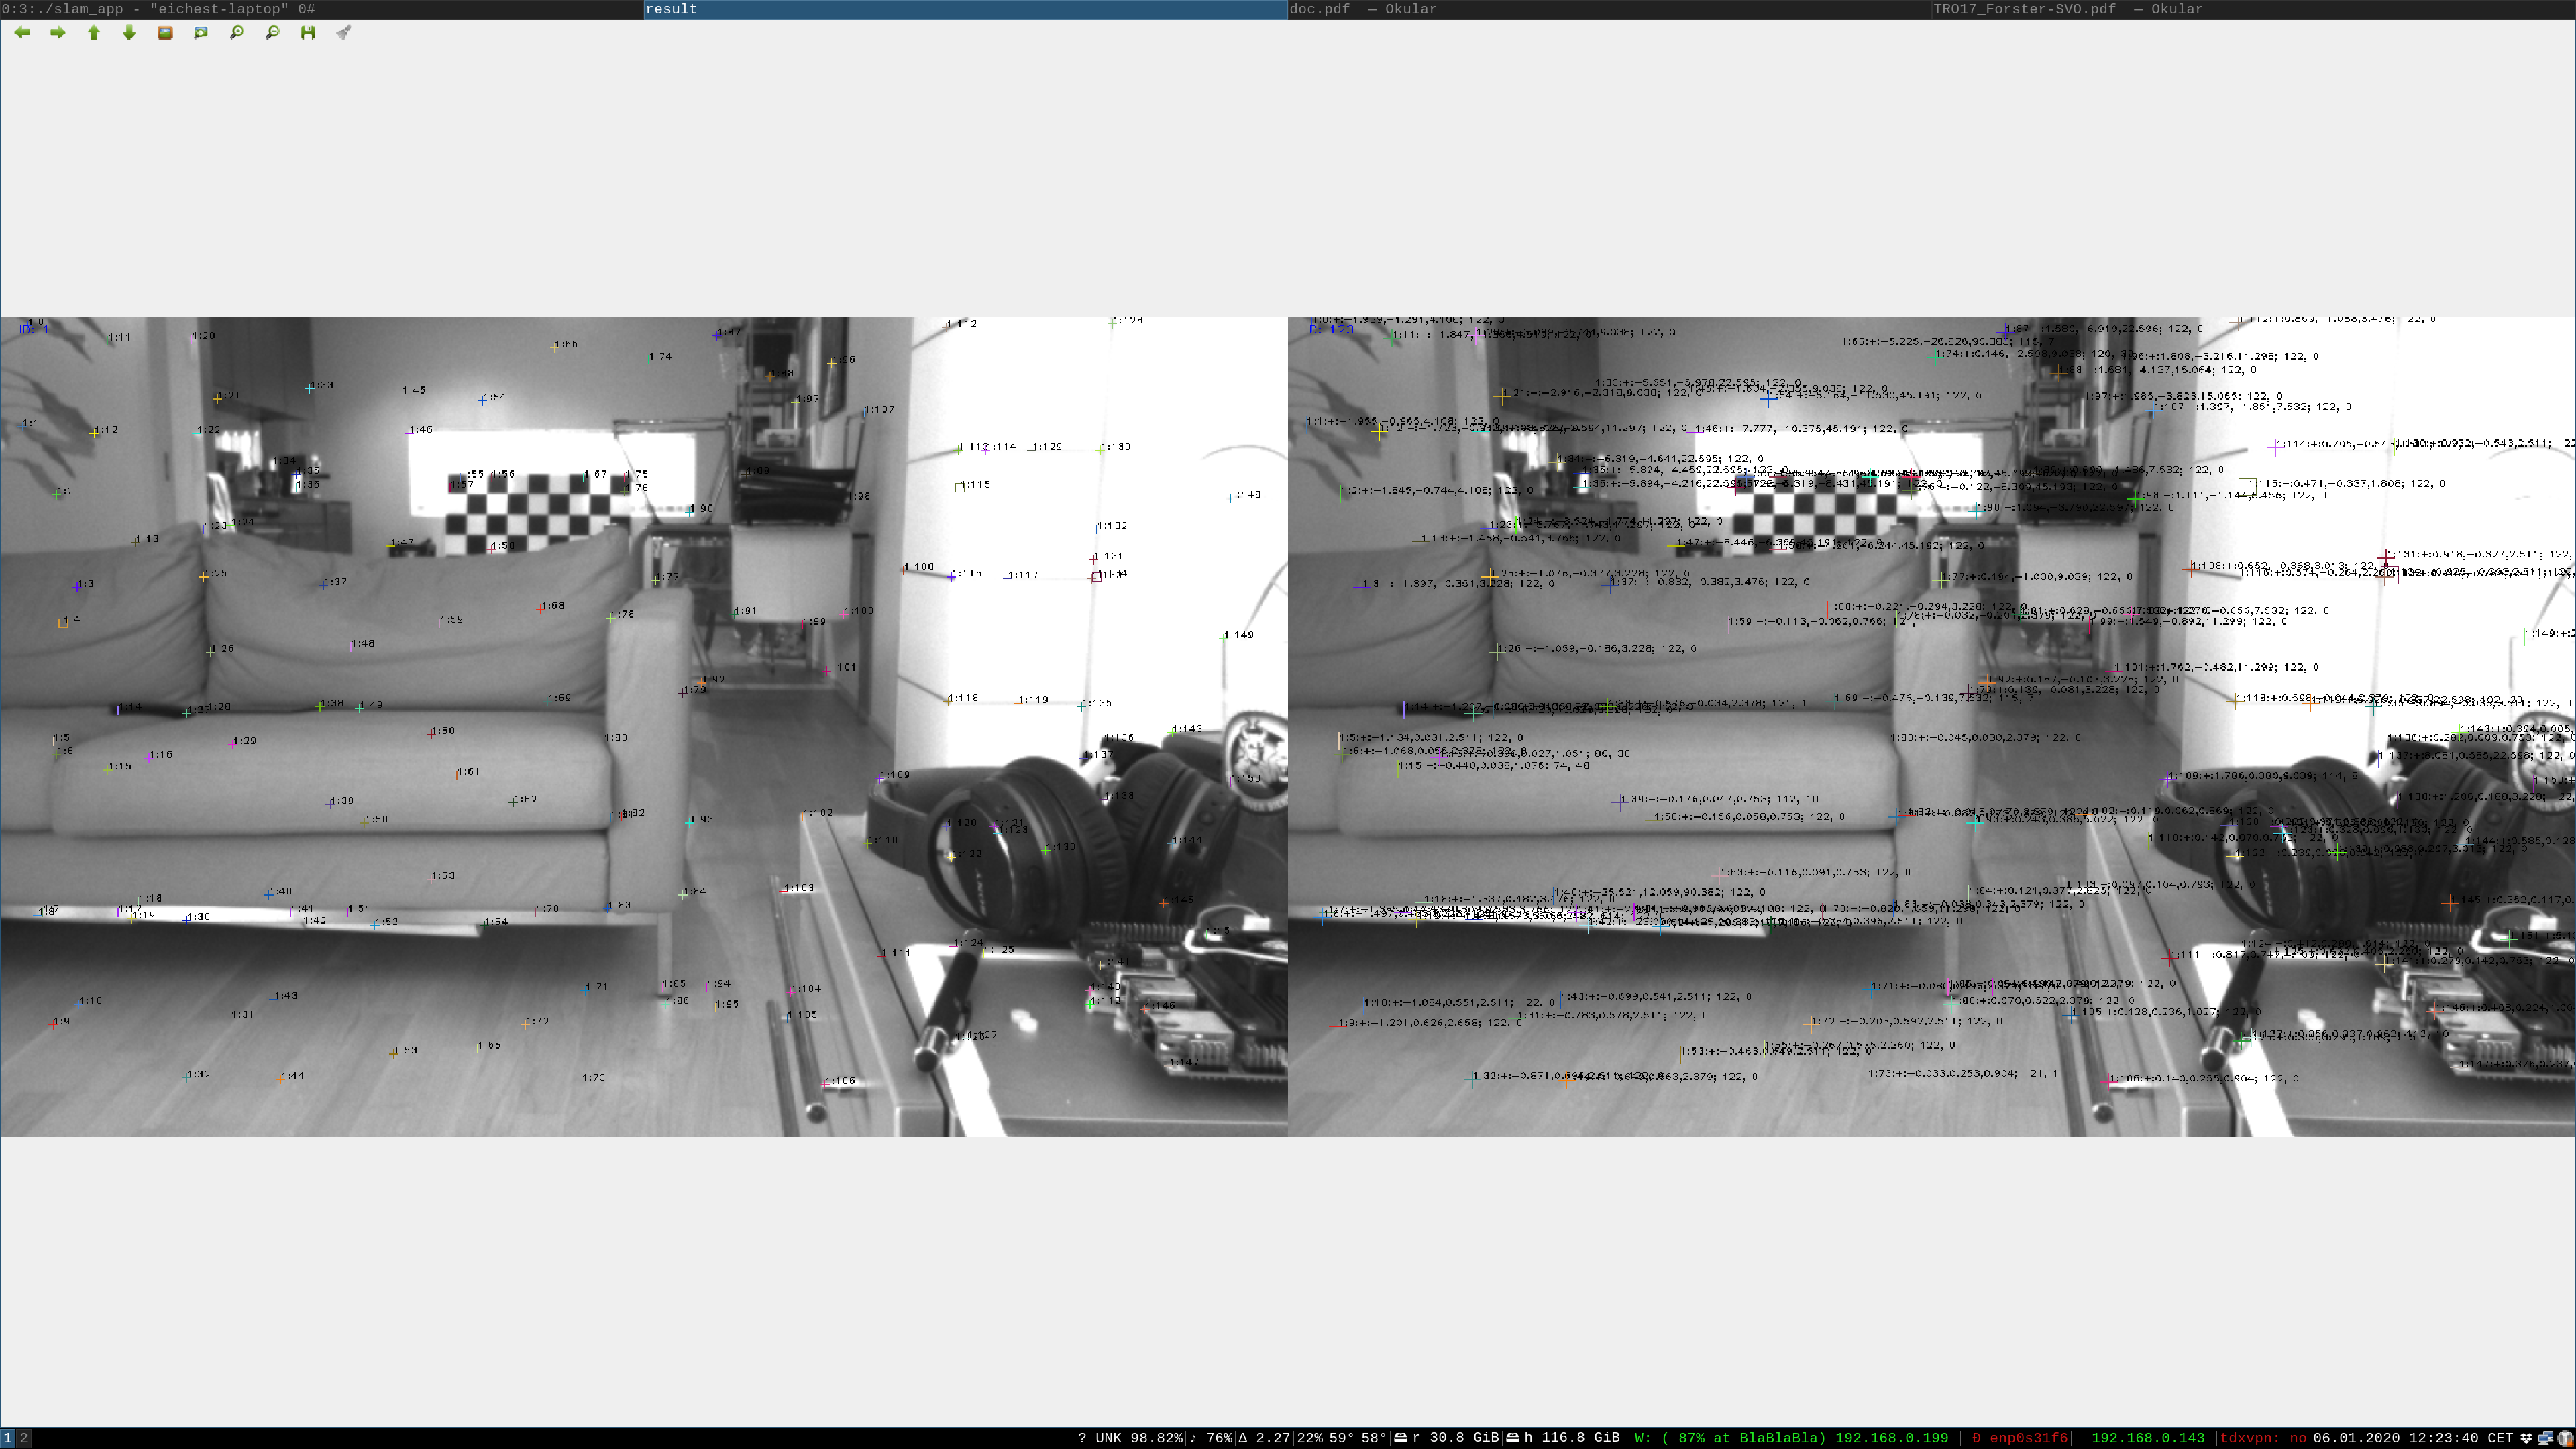
\includegraphics[width=0.9\textwidth]{img/test_app.png}
  \caption{Image from the Test Application}\label{fig:test_app}
\end{figure}

We can use the test application to test and debug the algorithm. It allows us to use different input sources like video, EuRoC and camera. Figure \ref{fig:test_app} shows an example of the output of the application. The left side shows the last keyframe with its keypoints. The right image shows the current frame. In the keyframe we show two numbers a:b. a is the keyframe id where the frame was first seen and b is the index of the keypoint in this keyframe. In the current frame it shows the information a:b:+/-:x,y,z;inliers,outliers. a and b are again the keypoint ids. + means the keypoint is currently used and - means the opposite. x,y,z are the 3D position and the last two numbers say how many times the point was counted as inlier or as an outlier. The numbers are small but it is possible to zoom in to make them bigger. These numbers are interesting when debugging the application. By pressing a key other than q we can freeze the output to analyse the current state. By pressing q we can quit the application.\\
Additionally, to the above output the test application offers a Websocket \cite{websocket} backend. Through this backend it is possible for the Qt Viewer to read 3D data like current pose, keyframes and trajectory. We show the Websocket idea in figure \ref{fig:websocket}.

\begin{figure}[H]
  \centering
  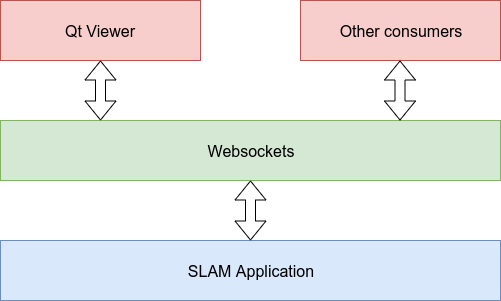
\includegraphics[width=0.9\textwidth]{img/websocket.png}
  \caption{Websocket Connection}\label{fig:websocket}
\end{figure}

Table \ref{tab:websocketapi} shows the implemented Websocket URLs and commands. For trajectory it will send x1, y1, z1, rx1, ry1, rz1, x2, y2, z2, \dots The test application will open a Websocket on port 8001.

\begin{table}[H]
  \centering
  \begin{tabular}{|l|l|l|}
    URL & Command & Response \\
    \hline
    keypoints & get & \makecell[l]{\{\\"colors":[\{"b":139,"g":69,"r":103\},\dots],\\"keypoints":[\{"x":-4.8,"y":-0.9,"z":6.1\},\dots],\\pose":\{"rx":0.4,"ry":0.1,"rz":-0.9,"x":-1.8,"y":0.2,"z":0.1\}\\\}}\\
    \hline
    pose & get & \makecell[l]{\{"pose":\{"rx":-9.1,"ry":0.0,"rz":-0.0,"x":-1.2,"y":0.0,"z":-2.0\}\}}\\
    \hline
    trajectory & get & \makecell[l]{\{"trajectory":[0,0,0,0,0,0,0.1,0.1,0.1,0.1,0.1,0.1,0.1,\dots]\}}\\
  \end{tabular}
  \caption{Websocket commands}
  \label{tab:websocketapi}
\end{table}

\section{Qt Viewer}
\begin{figure}[H]
  \centering
  \subfloat[Viewer with reduced keyframes]{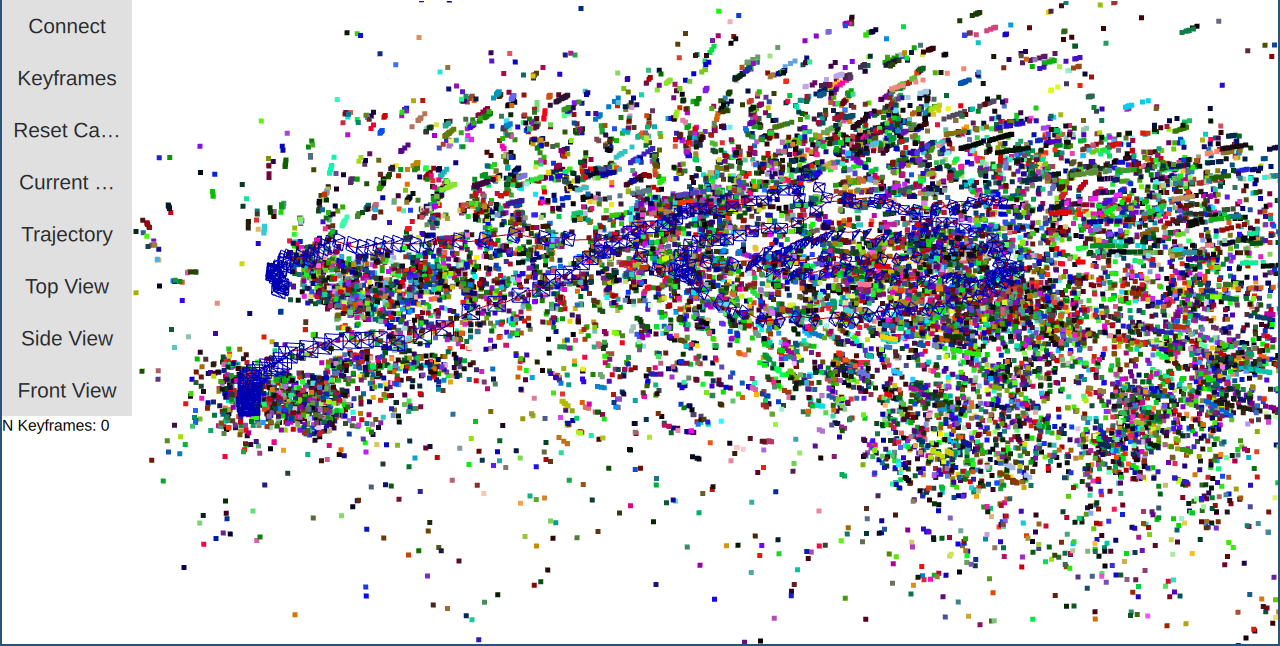
\includegraphics[width=0.45\textwidth]{img/qt_viewer1.png}}
  \qquad
  \subfloat[Viewer with all keyframes]{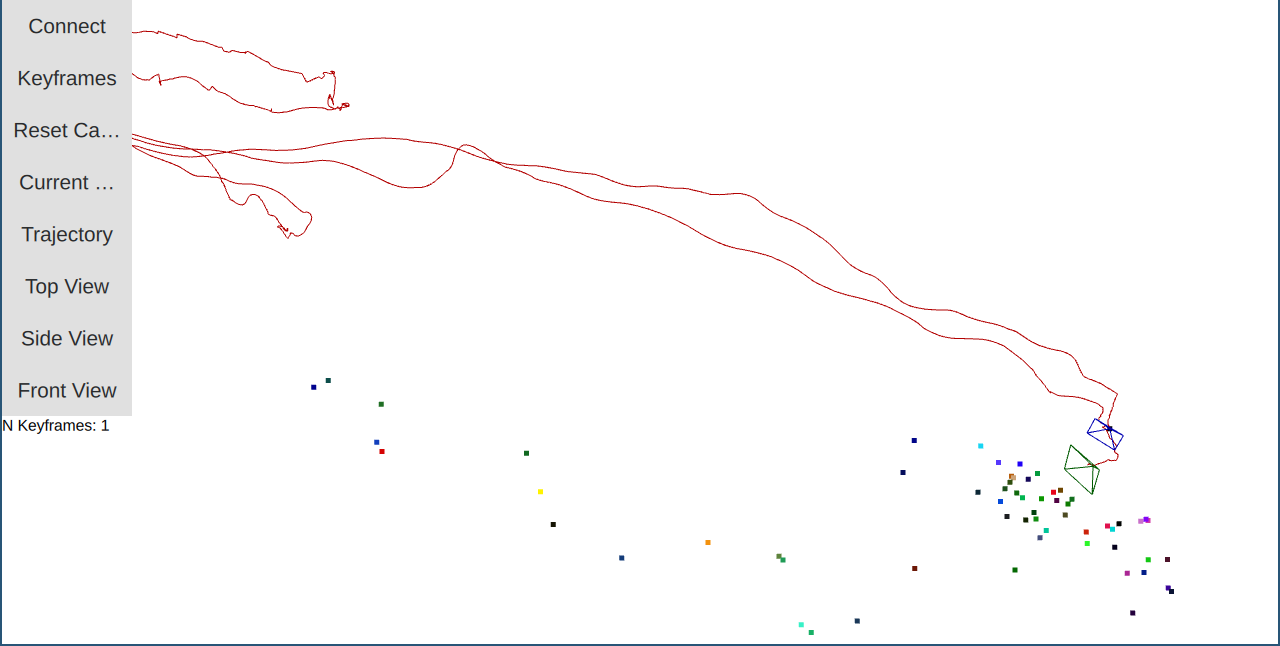
\includegraphics[width=0.45\textwidth]{img/qt_viewer2.png}}
  \caption{Qt Viewer}\label{fig:qt_viewer}
\end{figure}

We can use the Qt Viewer shown in figure \ref{fig:qt_viewer} to display 3D information calculated by the Test Application. We can navigate with the cursor to move trough the 3D room. The data is not received automatically. We need to click connect, get pose, etc. to trigger an action. This allows us to keep a snapshot of a scene and to analyse the current state. All points have the same color as displayed in the test application. Keyframes are shown as blue rectangles and the current frame pose is shown in green. The trajectory is shown as a red line. When pressing the connect button it will automatically connect to localhost on port 8001, which is where the Test Application is listening on.

\section{Demo application}
\begin{figure}[H]
  \centering
  \subfloat[Demo application first view]{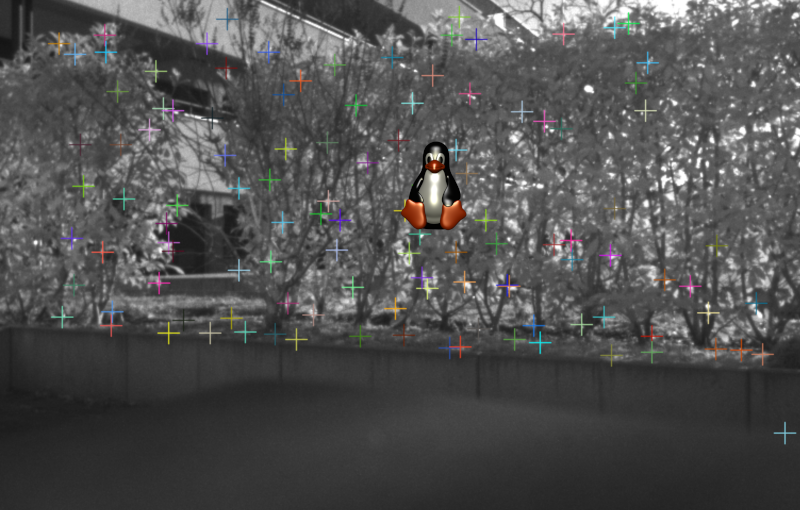
\includegraphics[width=0.45\textwidth]{img/demo_app1.png}}
  \qquad
  \subfloat[Demo application different view]{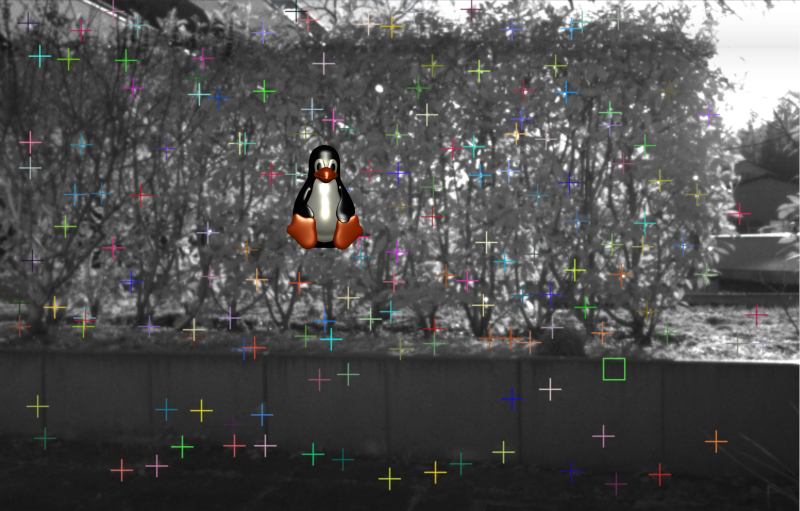
\includegraphics[width=0.45\textwidth]{img/demo_app2.png}}
  \caption{Demo Application}\label{fig:demo_application}
\end{figure}

The demo application shown in figure \ref{fig:demo_application} is a simple augmented reality application that demonstrates one usecase. If we move the camera, the Tux should stay at the same place. It is possible to disable the painting of the keypoints by not providing the -p option when starting the application. Only the econ camera is supported as input.

\section{Additional tools}

There are a few other tools available, but they will not be documented in more detail, because they are not intended for common use.

\subsection{Python wrapper}
There is a Python wrapper under src/python which uses Cython to generate bindings. It allows us to use libstereoslam from Python. We provide a demo application as main.py. It offers a similar feature set as the Test Application but it is slower.

\subsection{Scripts}
There are several scripts under test which we can use to record videos from the econ camera in the right format, to plot results, to export trajectory from Blender, etc.

\chapter{Results}\label{ch:results}

For testing the algorithm with a reference implementation we use two synthetic scenes generated by Blender. The advantage of having synthetic scenes is that we can test well defined movements where we know the trajectory. Blender allows to render stereoscopic videos by following the manual \cite{blender_stereo}. It is possible to customize the baseline, focal length in the camera settings of Blender. We can use the script test/blender-export-trajectory.py to export the camera trajectory into a csv file. This we can then use for comparison. The Test Application allows to export the trajectory of a scene by providing a -t argument.\\
We did all measurements in this chapter on an Intel i7-8550U processor. For our SVO implementation we use the settings in src/app/Blender.yaml. For SVO and SVO Edglet we adjusted fx,fy,cx and cy (see Blender.yaml) the rest is left unchanged. For ORB\_SLAM2 we use the settings found in test/ORB-Blender.yaml.

\section{Classroom}
\begin{figure}[H]
  \centering
  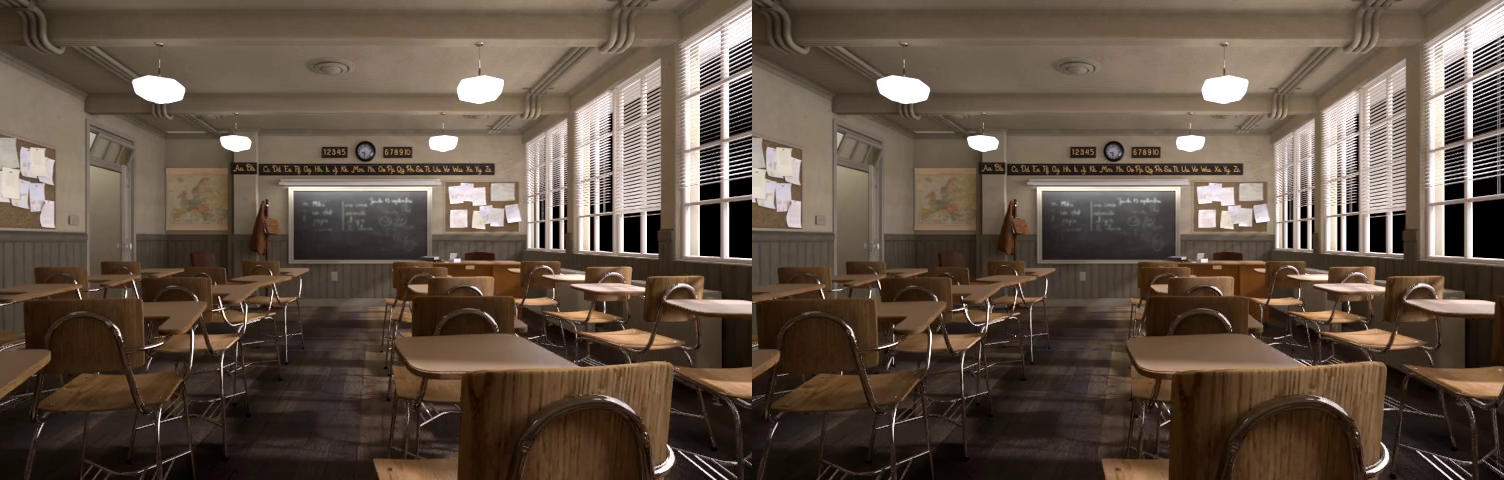
\includegraphics[width=1.0\textwidth]{img/blender_classroom_scene.png}
  \caption{Blender classroom scene}\label{fig:blender_classroom_scene}
\end{figure}

For the first test we use the Blender Classroom Scene \cite{blender}. We show a snapshot of this scene in figure \ref{fig:blender_classroom_scene}. An image for the left and right camera is rendered to have a valid stereo image input. We change the position and angles in the scene as shown in figure \ref{fig:blender_classroom_simple_traj}. The test video is part of the repository under test/blender-classroom.mkv. The trajectory file is called test/blender-classroom.csv. We compare our implementation with SVO \cite{svo}, SVO edgelet \cite{svo_edglet} and ORB SLAM \cite{orbslam}. SVO edgledt additionally uses edglets which are missing in the original SVO sources. Because SVO and ORB SLAM have dependencies to old libraries, we move the implementation to a Docker container. The Dockerfile is available in the test folder.

\begin{figure}[H]
  \centering
  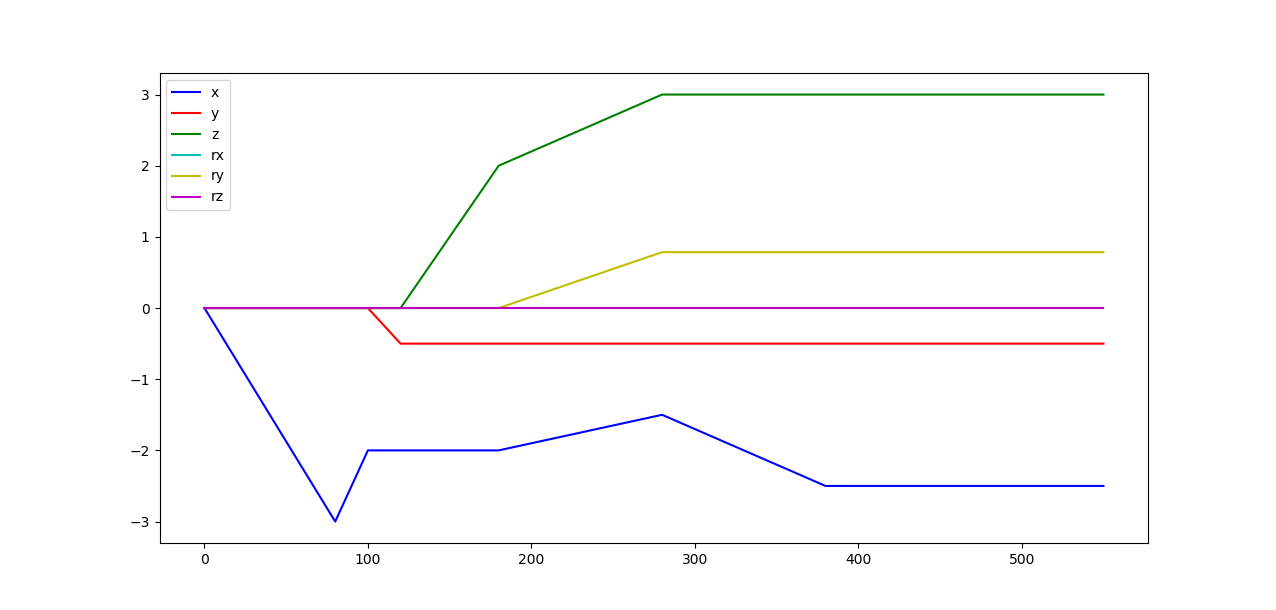
\includegraphics[width=1.0\textwidth]{img/blender_classroom_simple_traj.png}
  \caption{Blender classroom trajectory}\label{fig:blender_classroom_simple_traj}
\end{figure}

Figure \ref{fig:blender_classroom_simple_diff} shows the trajectory difference measured by our implementation, the SVO edgeled reference and the orignal SVO implementation. We scale both reference implementations to make a comparison possible. Table \ref{tab:maximas} shows the maximum error, table \ref{tab:average} the average error and table \ref{tab:fps} the average frames per seconds when doing the measurement. Figure \ref{fig:blender_classroom_comp} shows what we expect. Monocular SLAM is much less accurate than Stereo SLAM. While ORB SLAM matches the trajectory almost perfect, our implementation of SVO has a slight offset when tracking the transverse movement (figure \ref{fig:blender_classroom_comp}a).

\begin{table}[H]
  \centering
  \begin{tabular}{|c|c|c|c|c|c|c|}
    impl & err x & err y & err z & err rx & err ry & err rz\\
    \hline
    Our SVO & 0.031 & 0.013 & 0.073 & 0.205 & 0.610 & 0.285\\
    Edgled SVO & 0.344 & 0.099 & 0.273 & 0.989 & 12.941 & 1.430\\
    Original SVO & 0.300 & 0.120 & 0.488 & 1.169 & 6.123 & 1.390\\
    ORB SLAM& 0.023 & 0.015 & 0.023 & 0.222 & 0.302 & 0.204
  \end{tabular}
  \caption{Maximum errors in meter (x,y,z) and Degrees (rx,ry,rz)}
  \label{tab:maximas}
\end{table}

\begin{table}[H]
  \centering
  \begin{tabular}{|c|c|c|c|c|c|c|}
  impl & err x & err y & err z & err rx & err ry & err rz\\
  \hline
  Our SVO & 0.008 & 0.005 & 0.032 & 0.110 & 0.390 & 0.107\\
  Edgled SVO & 0.158 & 0.050 & 0.093 & 0.477 & 5.349 & 0.344\\
  Original SVO & 0.060 & 0.058 & 0.202 & 0.396 & 3.132 & 0.557\\
  ORB SLAM & 0.006 & 0.004 & 0.011 & 0.074 & 0.084 & 0.123
\end{tabular}

\caption{Average errors in meter (x,y,z) and Degrees (rx,ry,rz)}
\label{tab:average}
\end{table}

\begin{table}[H]
  \centering
  \begin{tabular}{|c|c|}
  impl & FPS\\
  \hline
  Our SVO & 52.38\\
  Edgled SVO & 0.93\\
  Original SVO & 115.81\\
  ORB SLAM & 17.38
\end{tabular}
\caption{Frame rate}
\label{tab:fps}
\end{table}

As we see in the results, tracking ry and z is specially challenging for monocular SLAM. Both are expected because by changing ry we can often correct small movements along the x axis. Further, when moving along the z axis we are not able to add new 3D points because we do not have a change along the x or y axis

\begin{figure}[H]
  \centering
  \subfloat[Our implementation]{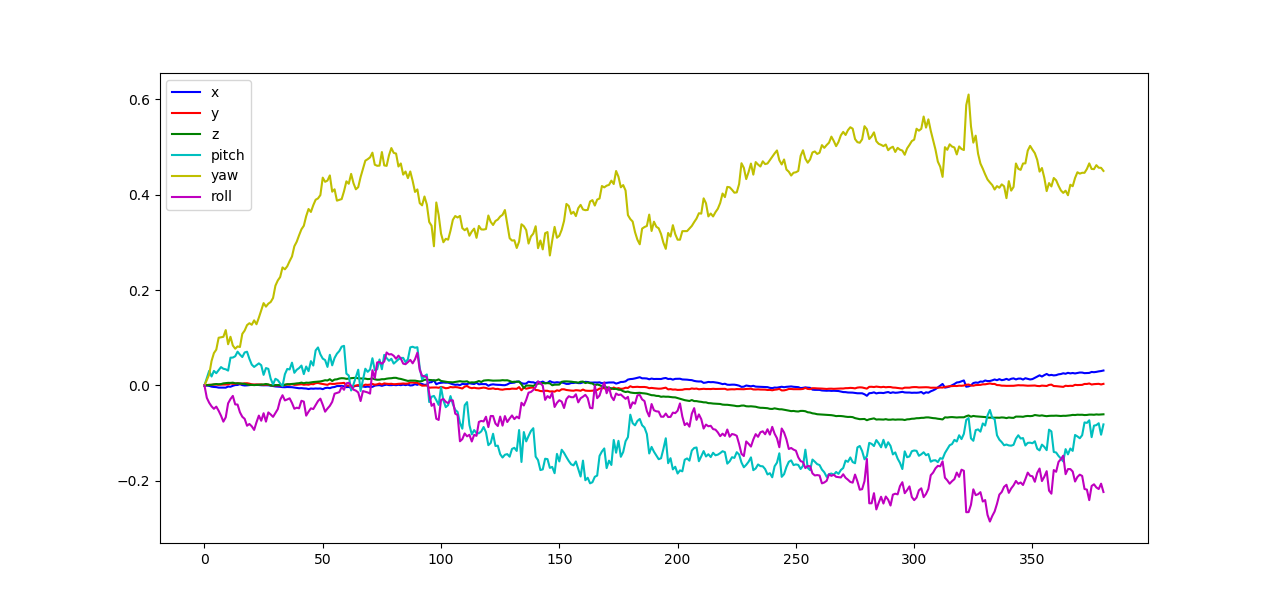
\includegraphics[width=0.7\textwidth]{img/blender_classroom_simple_our_diff.png}}\\
  \subfloat[SVO Edgled implementation]{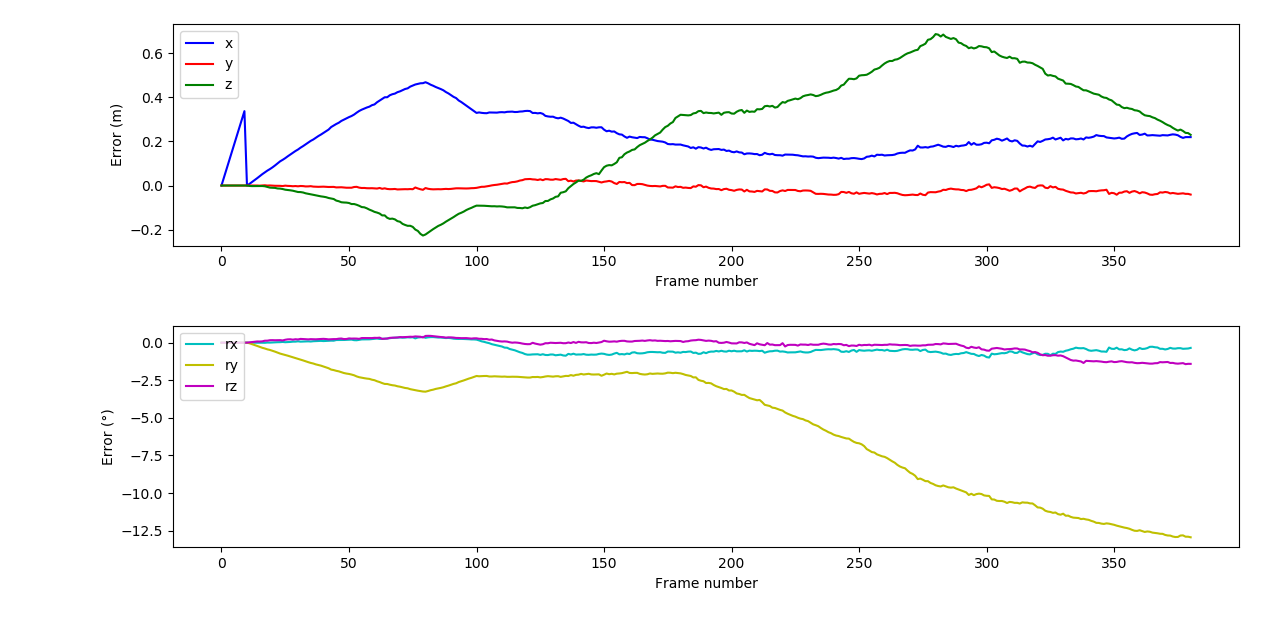
\includegraphics[width=0.7\textwidth]{img/blender_classroom_simple_ref_diff.png}}\\
  \subfloat[SVO Original implementation]{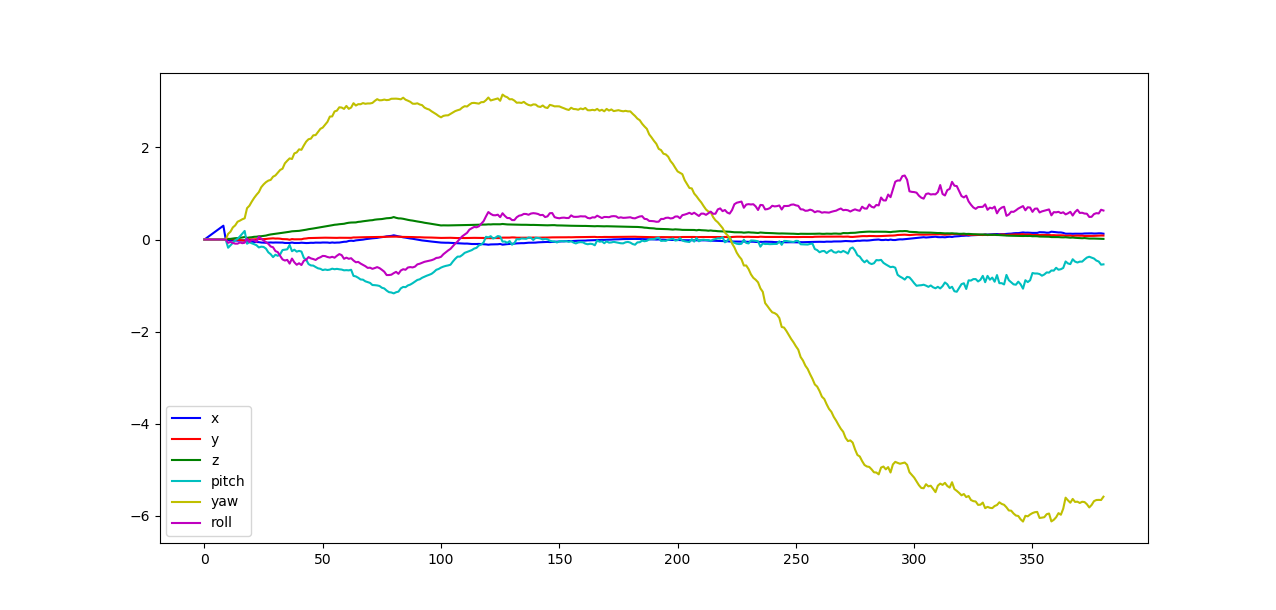
\includegraphics[width=0.7\textwidth]{img/blender_classroom_simple_orig_diff.png}}\\
  \subfloat[ORB SLAM]{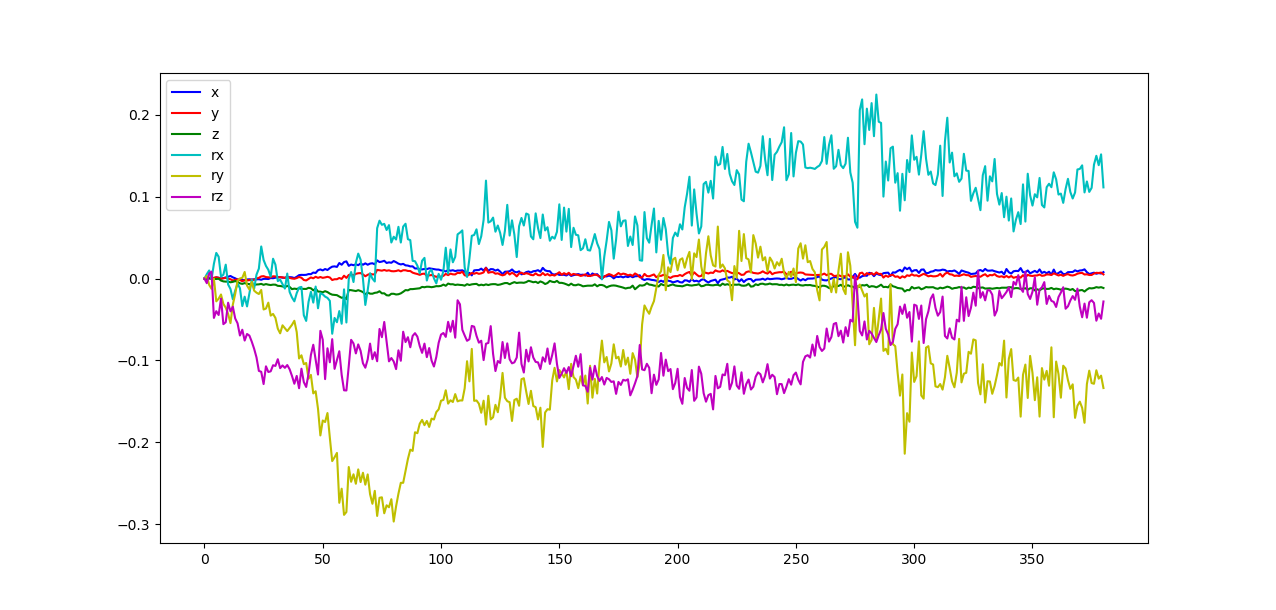
\includegraphics[width=0.7\textwidth]{img/blender_classroom_simple_orb_diff.png}}
  \caption{Blender Classroom scene errors}\label{fig:blender_classroom_simple_diff}
\end{figure}

\begin{figure}[H]
  \centering
  \subfloat[Top View]{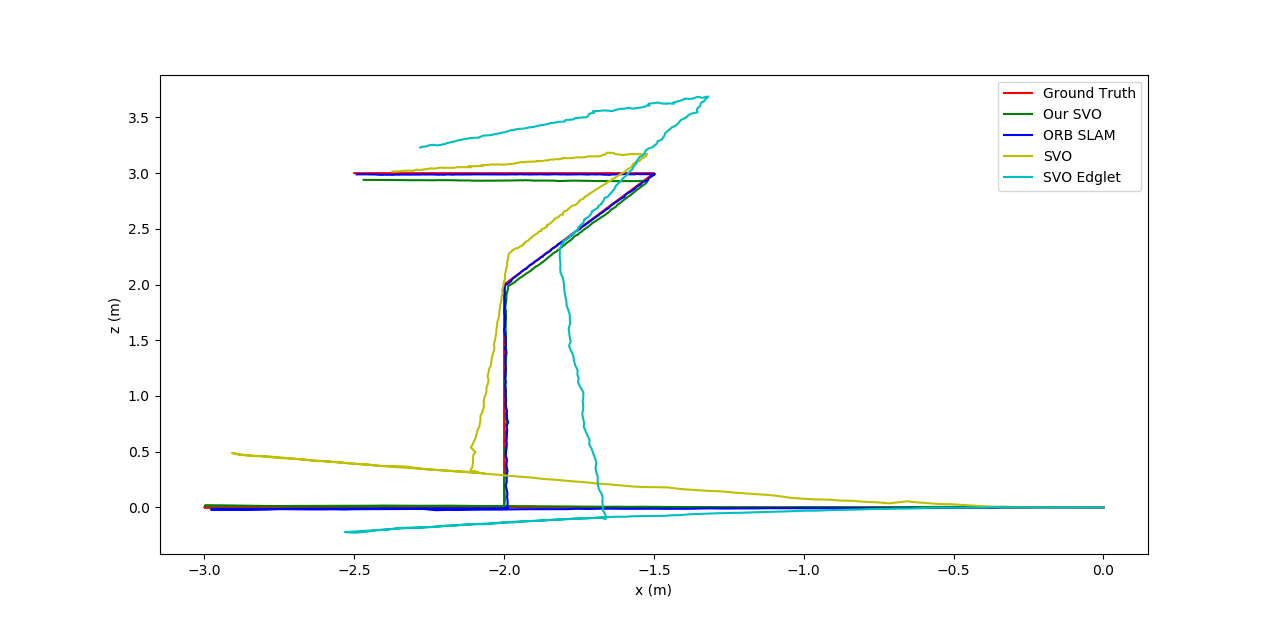
\includegraphics[width=0.9\textwidth]{img/blender_classroom_simple_comp_top.png}}\\
  \subfloat[Side View]{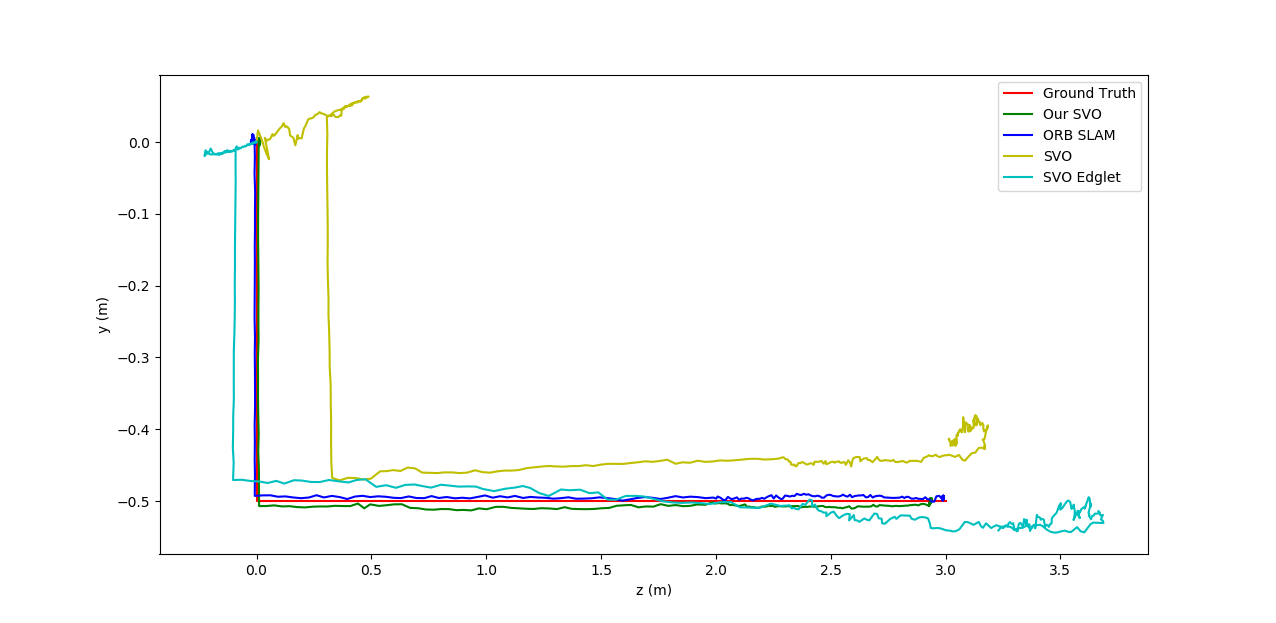
\includegraphics[width=0.9\textwidth]{img/blender_classroom_simple_comp_side.png}}
  \caption{Blender Classroom scene trajectory of our implementation, ORB, SVO and SVO Edglet}\label{fig:blender_classroom_comp}
\end{figure}

\section{Barcelona}

\begin{figure}[H]
  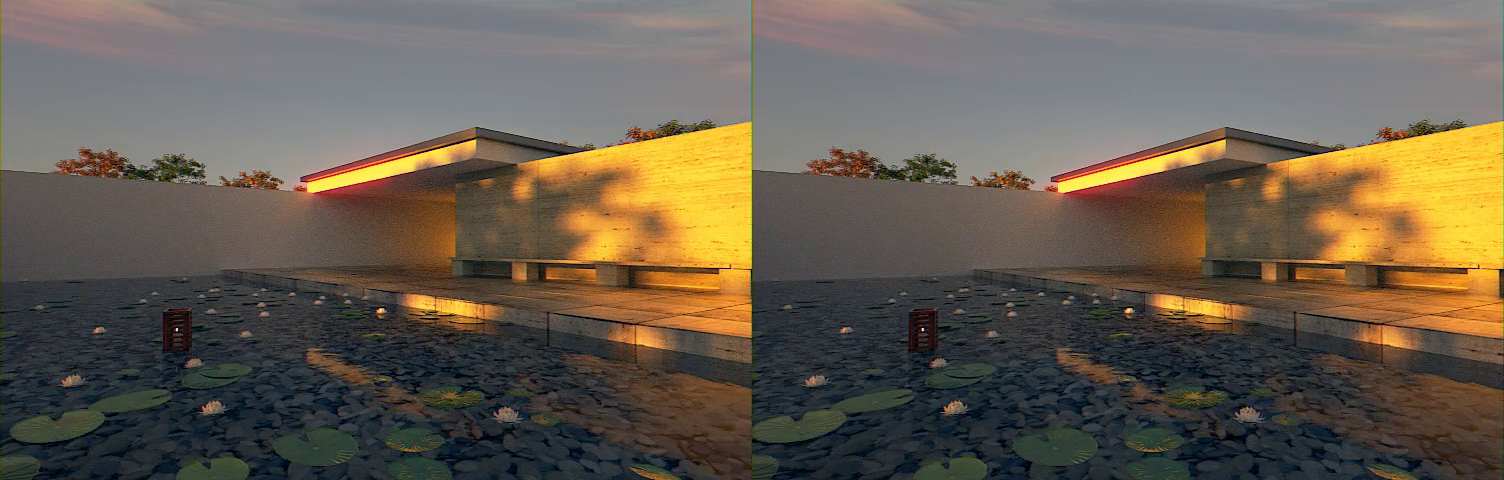
\includegraphics[width=1.0\textwidth]{img/blender_barcelona_scene.png}
  \caption{Blender Barcelona scene}\label{fig:blender_barcelona_scene}
\end{figure}

For the second test we use an outdoor synthetic scene called Barcelona \cite{blender}. Here we compare ORB SLAM with our SVO implementation because the monocular SLAMs are unable to track these movements. Figure \ref{fig:blender_barcelona_traj} shows the planned trajectory. The challenges for the tracker are movements along z axis and big changes in the angle. We can find the test video in the repository under test/blender-barcelona.mkv and the trajectory under test/blender-barcelona.csv.

\begin{figure}[H]
  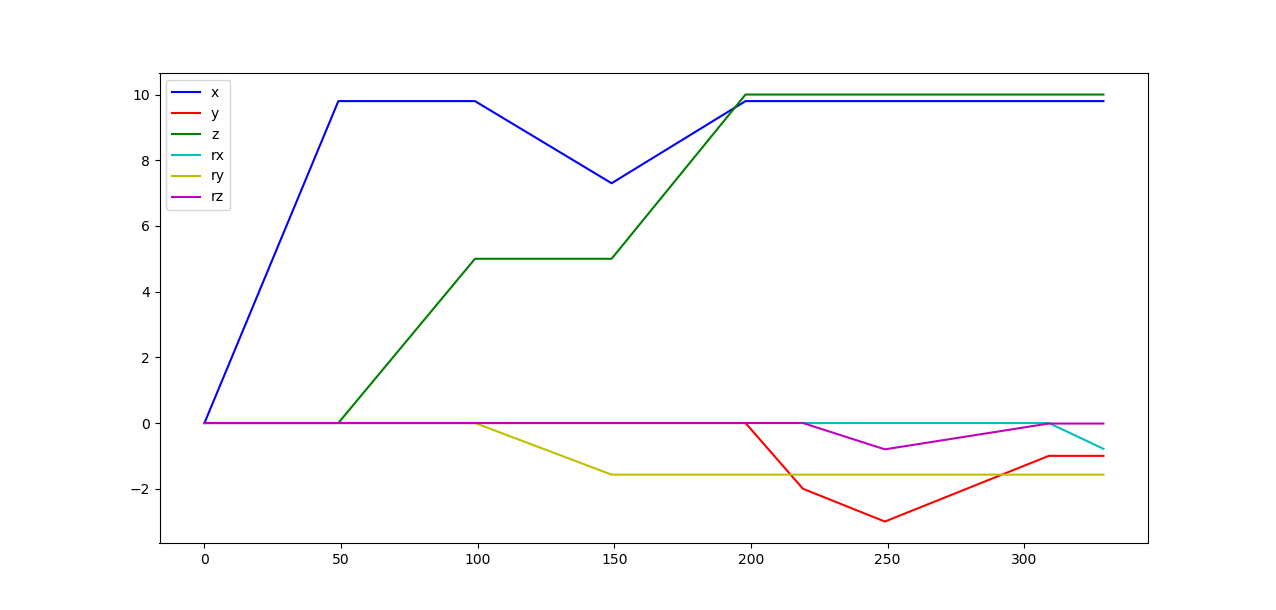
\includegraphics[width=1.0\textwidth]{img/blender_barcelona_traj.png}
  \caption{Blender Barcelona trajectory}\label{fig:blender_barcelona_traj}
\end{figure}

As we see in figure \ref{fig:blender_barcelona_diff}, both algorithms struggle for big angle changes without movement. When checking table \ref{tab:barcelona_maximas} and table \ref{tab:barcelona_average} we see that ORB SLAM performs slightly better but with a lower frame rate (table \ref{tab:barcelona_fps}) than our SVO SLAM implementation. Figure \ref{fig:blender_barcelona_comp}b shows that our algorithm has more problems to track movements along the y axis. It seems to track less abrupt changes than ORB SLAM in this scenario \ref{fig:blender_barcelona_comp}a.

\begin{table}[H]
  \centering
  \begin{tabular}{|c|c|c|c|c|c|c|}
  impl & err x & err y & err z & err rx & err ry & err rz\\
  \hline
  Our SVO & 0.622 & 0.537 & 0.956 & 10.417 & 11.222 & 14.682\\
  ORB SLAM& 0.993 & 0.189 & 0.592 & 7.491 & 19.315 & 10.542
\end{tabular}
\caption{Maximum error in meter (x,y,z) and Degrees (rx,ry,rz)}
\label{tab:barcelona_maximas}
\end{table}

\begin{table}[H]
  \centering
  \begin{tabular}{|c|c|c|c|c|c|c|}
    impl & err x & err y & err z & err rx & err ry & err rz\\
    \hline
    Our SVO & 0.396 & 0.166 & 0.451 & 1.012 & 2.753 & 2.446\\
    ORB SLAM & 0.734 & 0.088 & 0.416 & 0.711 & 2.717 & 1.955
  \end{tabular}
\caption{Average error in meter (x,y,z) and Degrees (rx,ry,rz)}
\label{tab:barcelona_average}
\end{table}

\begin{table}[H]
  \centering
  \begin{tabular}{|c|c|}
  impl & FPS\\
  \hline
  Our SVO & 39.56\\
  ORB SLAM & 22.53
\end{tabular}
\caption{Frame rate}
\label{tab:barcelona_fps}
\end{table}

\begin{figure}[H]
  \subfloat[Our implementation]{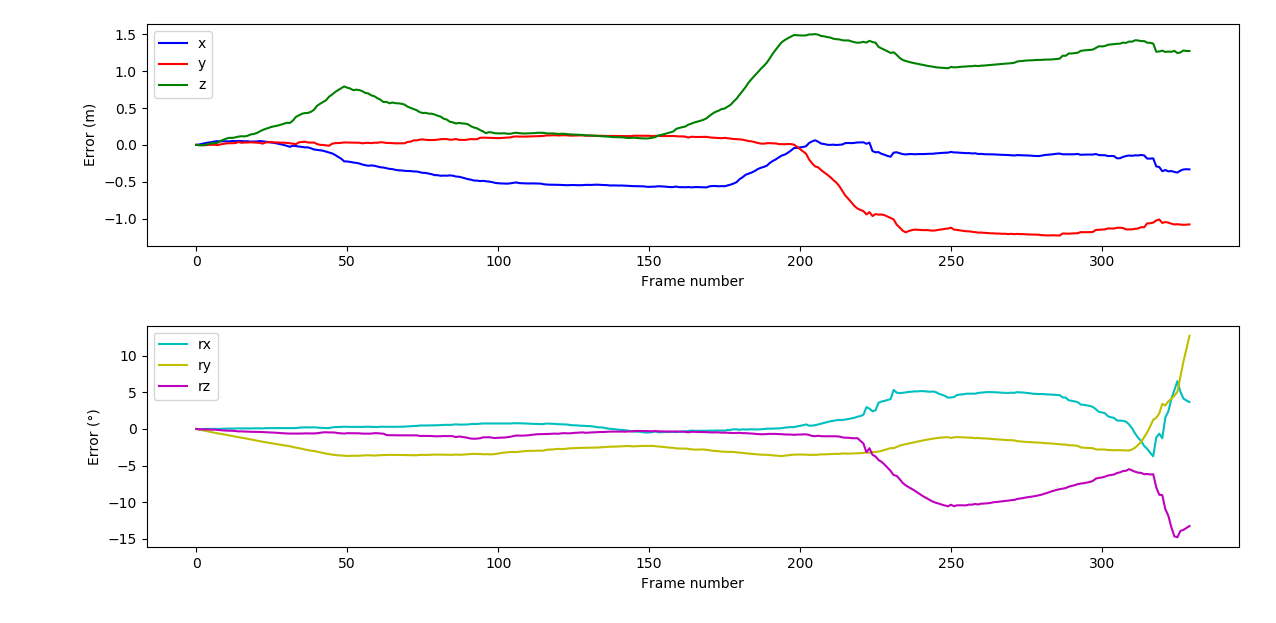
\includegraphics[width=0.9\textwidth]{img/blender_barcelona_our_diff.png}}\\
  \subfloat[ORB SLAM]{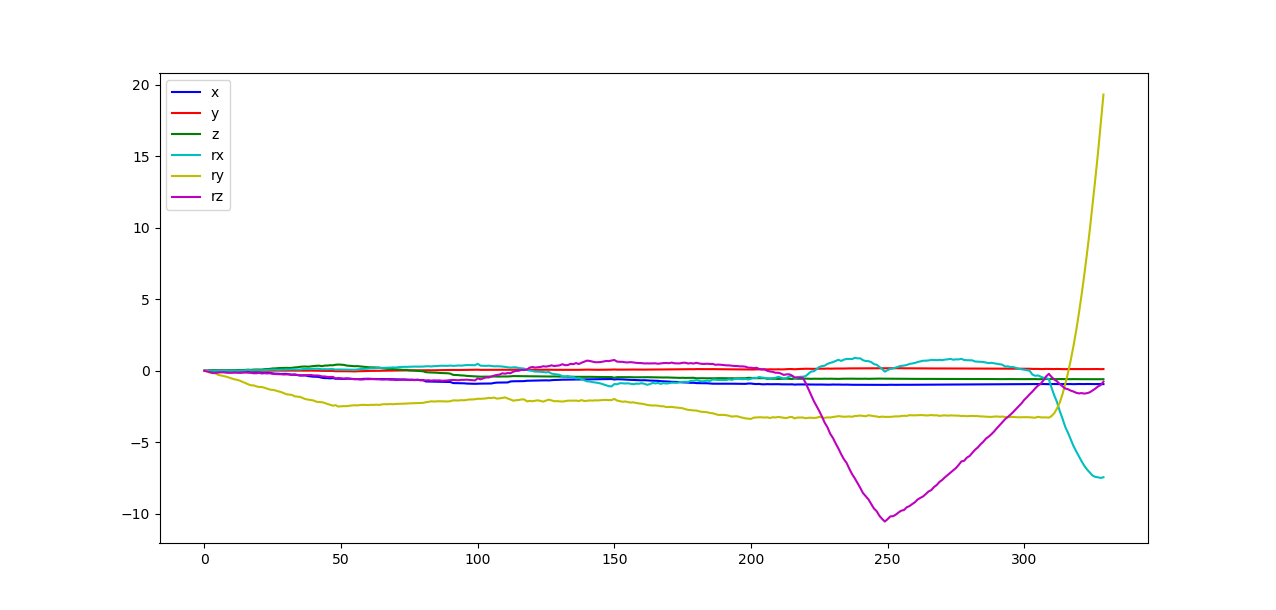
\includegraphics[width=0.9\textwidth]{img/blender_barcelona_orb_diff.png}}
  \caption{Blender Barcelona scene errors}\label{fig:blender_barcelona_diff}
\end{figure}

\begin{figure}[H]
  \centering
  \subfloat[Top View]{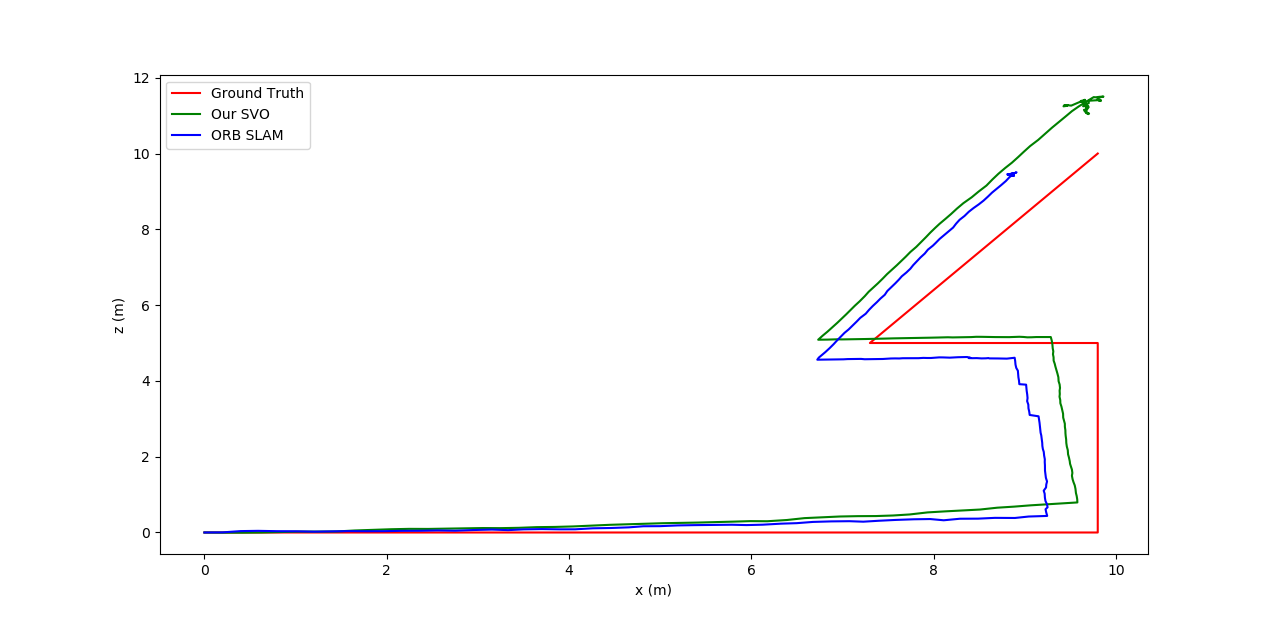
\includegraphics[width=0.9\textwidth]{img/blender_barcelona_comp_top.png}}\\
  \subfloat[Side View]{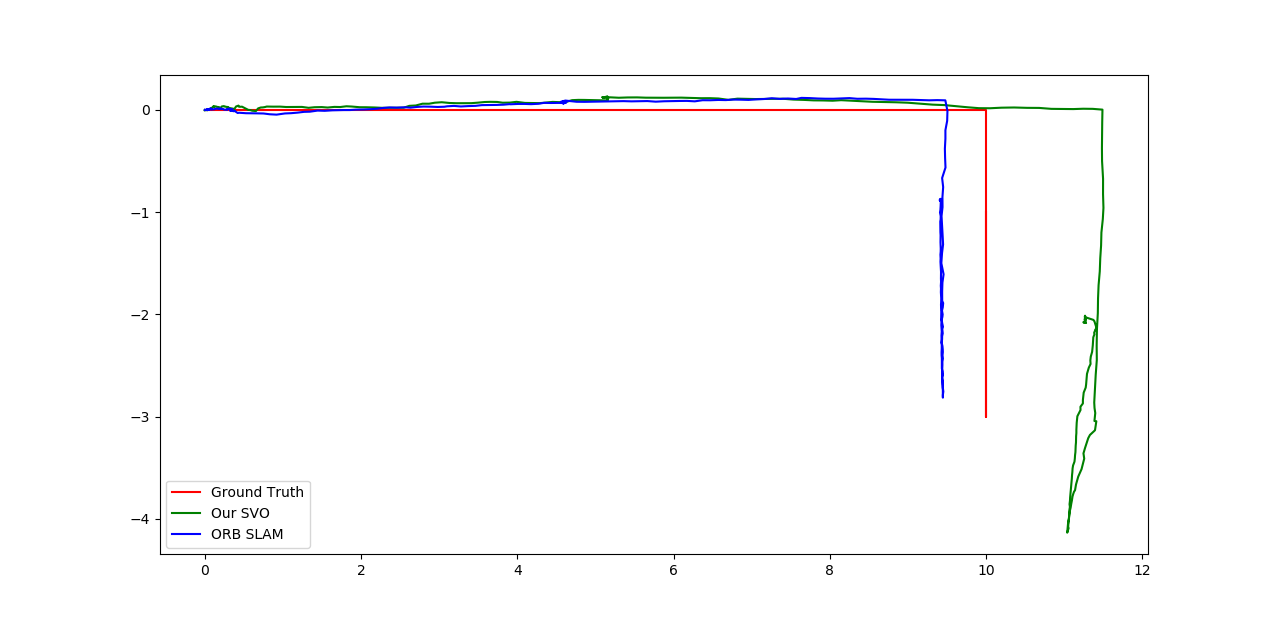
\includegraphics[width=0.9\textwidth]{img/blender_barcelona_comp_side.png}}
  \caption{Blender Barcelona scene trajectory of our SVO implementation and ORB}\label{fig:blender_barcelona_comp}
\end{figure}

\section{EuRoC Machine Hall 2}

\begin{figure}[H]
  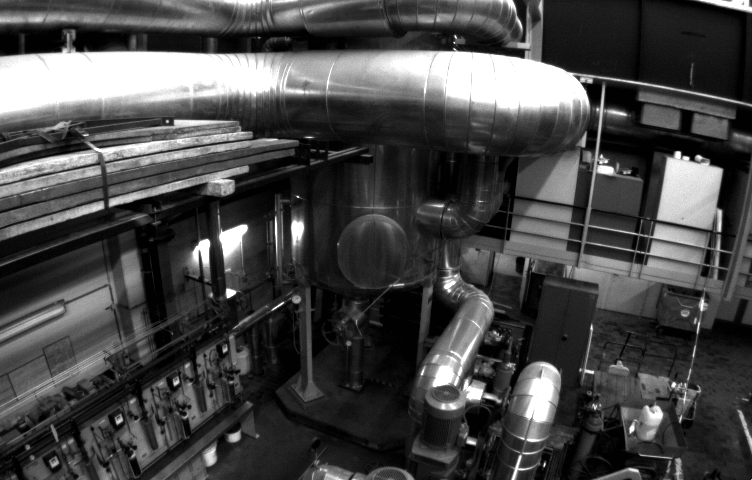
\includegraphics[width=1.0\textwidth]{img/euroc_scene.png}
  \caption{EuRoC Machine Hall 2 Scene}\label{fig:euroc_scene}
\end{figure}

EuRoC is a widely used dataset for SLAM algorithms \cite{euroc}. Figure \ref{fig:euroc_scene} shows an image from EuRoC Machine Hall 2. The SVO2 paper \cite{svo2} compares some measurements based on EuRoC. Our measurements are not in the range of any modern SLAM algorithm. The problem is that the current implementation doesn't do a relocation (local or global). Therefore, it can't profit if it sees the same scene more than once, what increases the drift. For completeness, an initial result is shown anyhow for EuRoC Machine Hall 2.

\begin{figure}[H]
  \subfloat[Top View]{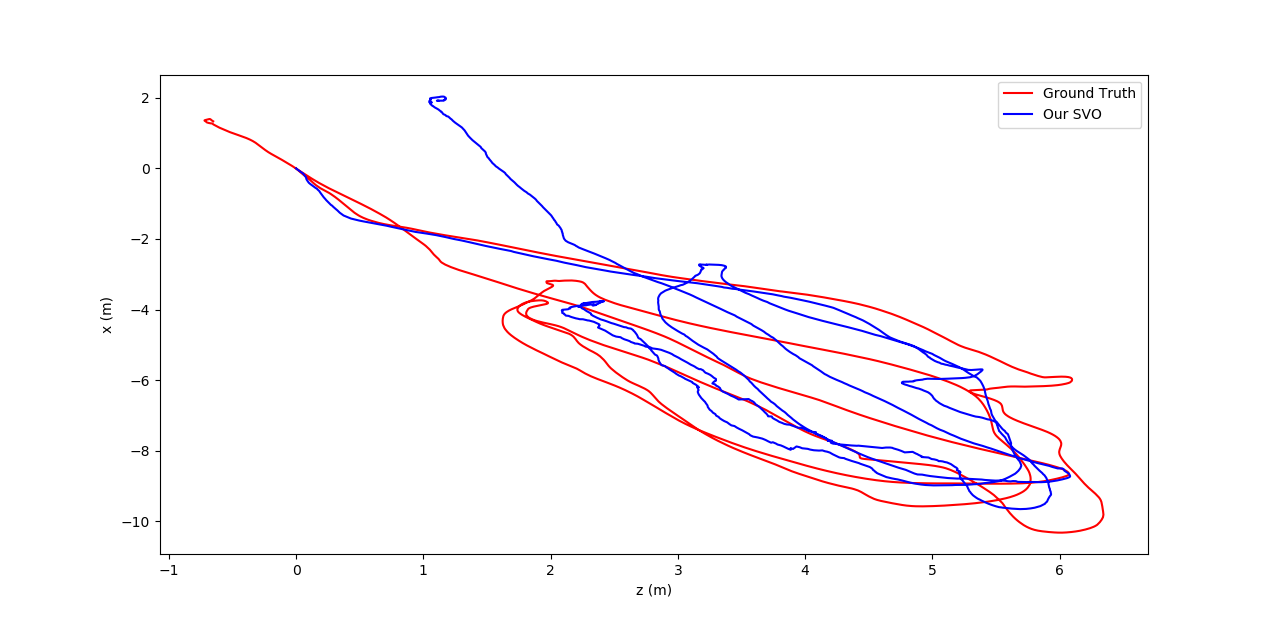
\includegraphics[width=0.9\textwidth]{img/euroc_svo_top.png}}\\
  \subfloat[Side View]{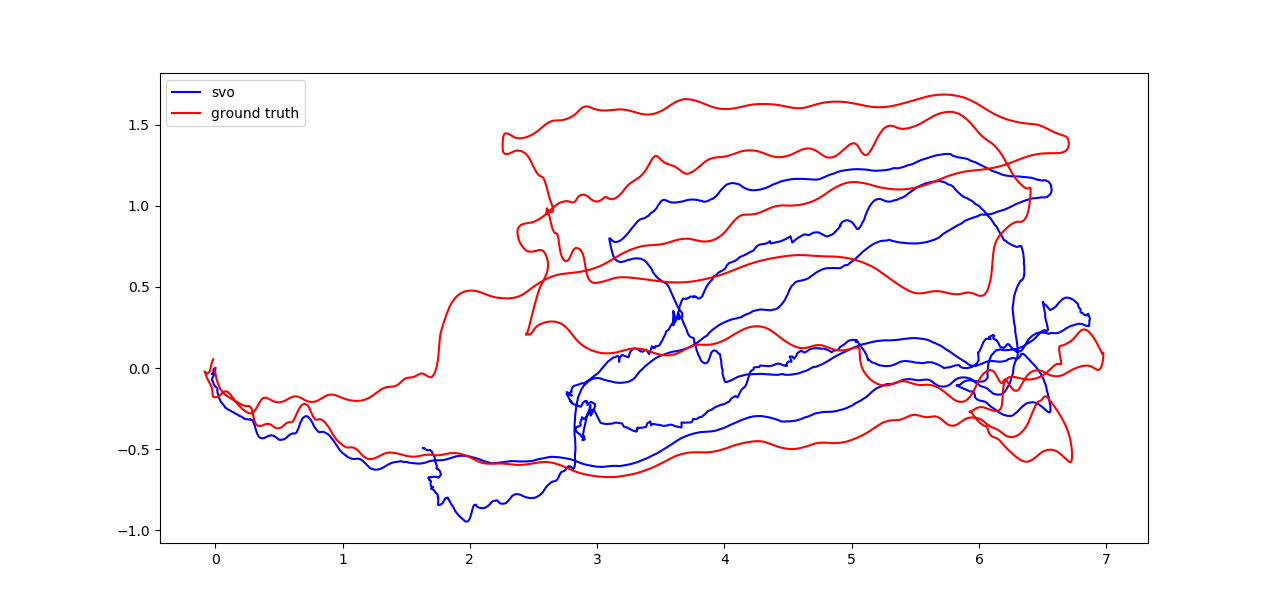
\includegraphics[width=0.9\textwidth]{img/euroc_svo_side.png}}\\
  \caption{EuRoC }\label{fig:euroc}
\end{figure}

As we see in figure \ref{fig:euroc} we have a huge drift over the whole sequence. We measure a final error of more than one meter in each direction. However, this was measured without doing a lot of parameters tuning. SVO2 states that they can achieve an RMSE of only 8 cm. SVO one, on which this thesis is based, can not follow the sequence at all. It is possible that we could achieve better results with our implementation by tweaking the parameters but it is unrealistic to get close to what SVO2 measured. The average frame rate was 37.13 fps.

\chapter{Discussion}\label{ch:discussion}

We showed that SVO works and is faster than e.g. ORB SLAM. Our implementation does not yet achieve the same frame rate as the reference implementation. However, by tweaking the source code, we should achieve higher frame rates. Some initial tests with OpenMP and TBB showed that the single-threaded version is faster. The task size per iteration is too low so that the overhead of multiprocessing is too large. By increasing the task size, we could probably improve this. However, more important seems to be to actively use vectorizations. By consistently using OpenCV vectors and matrices, the compiler can better optimize the code. We already gained at least a factor two by doing so. The depth filter implementation is the slowest part in the current implementation. However, it was also optimized the least. Therefore, we could gain the most by optimizing this part for the moment.\\\\
First tests on an ARM iMX8QM (Cortex A72) based system showed frame rates of 10fps for our SVO implementation and 5fps for ORB SLAM. However, here we didn't do any optimization or analysis yet. ARM NEON vectorizations is used by the compiler but we didn't do any function tracing on the library yet.\\\\
The accuracy of our implementation is lower than those of modern SLAM implementations. We could improve this by projecting old keypoints into the current frame to have some kind of local re-localization. We don't do that at the moment because of speed concerns and to keep the algorithm simple.\\\\
We implemented a 3D viewer which we can use over a network connections. This allows us to debug devices that are further away e.g. via Wifi or Ethernet. The current experience shows that this is a good approach because we can also separate the code base.\\\\
We showed an easy way to generate test scenes by using Blender animations. This allows us to debug easily. We know all movements and can add strict movements in one direction. Further it allows us to compare results between different algorithms and implementations. Generating scenes is simple, cheap and fast.\\\\
A demo application shows the possibilities of SLAM. It is a simple augmented reality application which we can use to showcase our algorithm.\\\\
The current library is in the state of a proof of concept. The implementation showed to be faster than ORB SLAM but it is not as robust yet. We can use the current state as a starting point for further development. The library is open source and has only dependencies to OpenCV. This makes it easier to compile it for other platforms and systems.\\\\
The CPVR lab currently uses ORB SLAM for its augmented reality projects. The benefit of SVO would only be performance-wise and not in terms of accuracy. Therefore, the effort to port its current projects to SVO doesn't seem to be justifiable. However, for future projects a combination of SVO and ORB SLAM could be an efficient solution for mobile devices. They could use SVO for tracking between frames, while ORB SLAM could do re-location. Inserting new keyframes and computing descriptors would still be done by ORB SLAM but the pose estimation would only involve sparse image alignment and pose refinement without triangulation. This could speed up the frame processing by a factor two.\\\\
We conclude that SVO shows great potential for use on embedded devices. The current implementation would need more tuning to achieve higher frame rates. However, we already showed that SVO runs faster than indirect SLAM algorithms like ORB SLAM.

\printbibliography

\end{document}
